\documentclass{aims}

%%%%%%%%%%%%%%%%%%%%%%%%%%%%%%%%%%%%%%%%%%
\usepackage{txfonts}
\usepackage{cite}
\usepackage{multirow,makecell}
\newcolumntype{C}[1]{>{\centering\arraybackslash}m{#1}}
\newcolumntype{L}[1]{m{#1}}
\usepackage{graphicx}
\usepackage{amsmath}
\usepackage{amssymb}
\usepackage{subfigure}
\usepackage{url}
\usepackage{xcolor}
\usepackage{soul}

\def\typeofarticle{Research article}
\def\currentvolume{11}
\def\currentissue{1}
\def\currentyear{2026}
\def\currentmonth{Received date 15 December 2025, Accepted date 23 January}
\def\ppages{xxx--xxx.}
\def\DOI{ 10.3934/math.2026xxx}
\def\Received{15 December 2025}
\def\Revised{17 January 2026}
\def\Accepted{23 January 2026}
\def\Published{xx January 2026}
\usepackage{cite}
\hyphenpenalty=10000
\setcounter{page}{1}

\numberwithin{equation}{section}
\DeclareMathOperator*{\essinf}{ess\,inf}
\makeatletter
\renewcommand{\@biblabel}[1]{#1\hfill \hspace{-0.2cm}}
\makeatother

\newcommand{\ep}{\varepsilon}
\newcommand{\eps}[1]{{#1}_{\varepsilon}}

\begin{document}

\title{Precaching vehicle selection based on soft actor-critic in CIoV}

\author{%
  Youngju Nam\affil{1},
  Yongje Shin\affil{2},
  Hyeonseok Choi\affil{3}
  and
  Euisin Lee\affil{4,}\corrauth
}

% \shortauthors is used in copyright information in the end of the paper
\shortauthors{the Author(s)}

\address{%
  \addr{\affilnum{1}}{School of Software, Kunsan National University, 54150, South Korea}
  \addr{\affilnum{2}}{Research Institute for Computer and Information Communication, Chungbuk National University, 28644, South Korea}
  \addr{\affilnum{3}}{Department of Computer Engineering, Seowon University, 28674, South Korea}
  \addr{\affilnum{4}}{School of Information and Communication Engineering, Chungbuk National University, 28644, South Korea}}

% corresponding author
\corraddr{Email: eslee@cbnu.ac.kr.}

\begin{abstract}
The rapid development of the Internet of Vehicles and the increasing demand for mobile content services have significantly increased network traffic, leading to congestion and delays. To address these challenges, Content-centric IoV has emerged by integrating IoV with Content-Centric Networking, enabling efficient mobile content delivery. However, CIoV still faces limitations in outage zones where roadside unit coverage is restricted, hindering content transmission. To overcome this issue, we propose a SAC-based Precaching Vehicle Selection scheme that dynamically selects optimal precaching vehicles and determines appropriate content sizes to facilitate content delivery in outage zones. SAC-PVS operates on a snapshot-based inference model, which is specifically designed to optimize precaching decisions at the exact moment of a request without relying on continuous time-series monitoring. It leverages the SAC algorithm to handle continuous action spaces, enabling precise determination of both the optimal caching vehicles and the corresponding content quantities. A hierarchical reward structure penalizes excessive caching and traffic waste while rewarding successful content delivery in outage zones. Simulation results demonstrate that SAC-PVS outperforms both a comparable machine learning approach and a non-machine-learning baseline by reducing content delivery latency and minimizing traffic waste under dynamic vehicular conditions. The proposed SAC-PVS scheme improves the Quality of Service for vehicle users and optimizes network resource utilization for content delivery, offering a scalable and efficient solution for next-generation CIoV content services.
\end{abstract}

\keywords{{content centric internet of vehicles; content precaching; vehicle-to-vehicle; soft actor critic; reinforcement learning}
\newline
\textbf{Mathematics Subject Classification:} 68M20, 68T05, 68T10, 90C40, 90C35}

\maketitle

\section{Introduction}
With the rapid development of the Internet of Vehicles (IoV), vehicles are becoming increasingly interconnected, forming a network of smart vehicles equipped with sensors, GPS, and on-board units~(OBUs). This interconnectivity enables vehicles to take advantage of enhanced functionalities, such as automated driving, real-time navigation, and communication with other vehicles and roadside units~(RSUs). With the advent of autonomous driving systems, passengers no longer need to focus on driving in IoV, allowing them to use their travel time for entertainment or productivity, which in turn increases the demand for high-quality content \cite{yuan2018}. However, this surge in data traffic within IoV is becoming a critical challenge. According to the Ericsson Mobility Report \cite{Ericsson}, global mobile data traffic was measured at 129 EB per month in 2022 and is expected to increase to 472 EB per month by 2028, representing a 3.66-fold growth. This dramatic increase in data demand may create significant congestion in IoV environments, leading to network bottlenecks and delays. As data traffic continues to grow, network infrastructures will struggle to maintain efficient content delivery. This will result in delays, similar to those currently experienced in densely populated areas such as airports or city centers \cite{Pranav2019}. Such delays in content delivery can significantly impact the Quality of Experience (QoE) for vehicle users who consume high-quality media, such as movies or YouTube videos, leading to frustration and dissatisfaction. Furthermore, these delays pose a more critical threat when real-time data are required for safety-critical services such as driving assistance and navigation. In such cases, delays in information transmission have the potential to compromise passenger safety in self-driving vehicles, thereby turning an otherwise efficient network into a persistent safety risk \cite{Reichardt2002}.

To address the growing demand for data in IoV environments, Content-Centric Networking (CCN) has been integrated into IoV, forming the Content-Centric IoV (CIoV) paradigm \cite{Li2017, Khan2024}.
Unlike traditional IP-based networks, where data are routed based on the IP addresses of the source and destination, CCN focuses on the content itself, allowing nodes to retrieve data based on content names rather than IP addresses. Owing to this unique characteristic of CCN, CIoV allows each vehicle and RSU to act as a caching node that can store frequently requested content locally. This reduces the need for vehicles to repeatedly receive content directly from content servers, thereby reducing latency and network congestion. The key advantage of CCN lies in its ability to distribute popular content closer to users, improving the efficiency of data delivery, especially in dynamic network environments such as CIoV, where connectivity can be intermittent.
A promising strategy within CIoV to further reduce latency and improve content availability is precaching, whereby content is preloaded at anticipated locations along a vehicle's route.
By predicting vehicle mobility and content requests, the network can cache content at RSUs before it is actually requested. This minimizes the need to access content servers in real-time, reducing delays and buffering. However, despite the benefits of precaching, the cost of~RSU deployment poses a significant challenge. Deploying RSUs across vast geographical area might be of high cost, resulting in the creation of outage zones that are located beyond the RSU coverage area \cite{Ahmed2018, Wang2021}. In these outage zones, vehicles may experience difficulties accessing cached content, leading to longer delays and reduced content availability. As a result, precaching at RSUs alone is insufficient to guarantee seamless content delivery in areas with limited RSU infrastructure.

As a solution for outage zones, the vehicle-to-vehicle (V2V) precaching approach has been proposed, in which vehicles share cached content with nearby vehicles \cite{Wang2017, Guo2017}. V2V precaching allows vehicles to act as mobile caching nodes, effectively expanding the network’s caching capacity and providing a more resilient content delivery system. This approach helps maintain content availability even in outage zones, as vehicles passing through these area can continue to receive content from caching vehicles without relying on RSUs. In V2V precaching, one of the most challenging issues is selecting appropriate vehicle to precache and deliver content. The selection of poor precaching vehicles can lead to inefficiency in precaching performance, as some vehicles may not have sufficient caching storage or may not encounter the content requester vehicle in time to deliver content. Consequently, accurate prediction of vehicle routes and content demand is critical to the success of V2V precaching, as selecting the wrong vehicles could result in delayed or failed content delivery, negating the benefits of the system. Existing studies still exhibit limitations in selecting the optimal precaching vehicles, as they primarily rely on predictions derived from simplistic mathematical models. Recently, the technology of Machine Learning (ML) has been applied to precaching in some studies \cite{Zhang2024, Chen2024}. However, these efforts have mainly focused on predicting whether content should be cached, without addressing more complex scenarios such as precaching vehicle selection in outage zones or predicting the precaching size for each vehicle.
Moreover, they do not fully consider vehicle connectivity dynamics and their impact on content delivery efficiency. Therefore, a significant gap remains in leveraging ML to optimize V2V precaching performance in outage zones, especially in jointly predicting optimal precaching vehicles and suitable content sizes to enable seamless content delivery. To the best of our knowledge, this is the first study to apply ML to optimize V2V precaching specifically in outage zones.

In this paper, we introduce a novel SAC-based V2V precaching scheme that leverages the advanced capabilities of the Soft Actor-Critic (SAC) algorithm and integrates key insights from recent studies to overcome the limitations of existing ML-based precaching schemes. The proposed scheme employs SAC to jointly optimize both the selection of precaching vehicles and the allocation of content by exploiting its inherent ability to handle continuous action spaces which is a critical feature for accurately identifying the optimal caching candidates and determining the precise quantities of content to be cached. Unlike existing schemes that treat these decisions in isolation, our scheme seamlessly incorporates real-time mobility patterns, connectivity metrics, and data provided by RSUs to dynamically adjust precaching strategies. It ensures robust content delivery even in challenging outage zones.
Specifically, we propose a snapshot-based inference approach that optimizes precaching decisions at the exact moment a request occurs, thereby avoiding the overhead and delay sensitivity associated with continuous time-series monitoring. Moreover, by leveraging SAC’s off-policy learning mechanism through a replay buffer, the proposed scheme efficiently reuses past experiences, significantly enhancing sample efficiency and accelerating convergence compared with on-policy approaches such as PPO. The incorporation of entropy regularization further enables a balanced trade-off between exploration and exploitation, preventing premature convergence and allowing the model to continuously refine its decisions under varying vehicular conditions. Extensive simulation results validate our approach, demonstrating that our SAC-based scheme not only significantly reduces content download delays but also minimizes wasted network resources, ultimately leading to improved Quality of Services (QoS) for vehicle users and provides superior adaptability to dynamic network environments for support content delivery in CIoV.

The remainder of this paper is organized as follows. Section~\ref{sec.rw} reviews related work on precaching and machine learning approaches in vehicular networks. Section~\ref{sec.nm} details the network models and provides an overview of the proposed system. Section~\ref{sec.prop} describes the SAC-based Precaching Vehicle Selection (SAC-PVS) scheme, outlining its design and implementation. Section~\ref{sec.perf} presents a comprehensive performance evaluation through extensive simulations, comparing our approach to baseline methods. Section~\ref{sec.disc} discusses potential directions for future research, and Section~\ref{sec.conc} concludes the paper.


\section{Related work} \label{sec.rw}
In the current Internet of Vehicles (IoV) paradigm, content downloading faces significant challenges due to reliance on IP address-based routing, which becomes problematic as vehicles often move at high speeds. When multiple vehicles within the coverage area of an RSU request the same content, the traditional IP-based routing method processes each request individually by establishing separate connections between the content server and the RSU where the vehicles are located. This approach results in more than double the necessary traffic load on backhaul links. Furthermore, frequent handovers caused by the high speeds of vehicles exacerbate access delays, as each time a vehicle enters a new RSU's coverage area, a new request is sent to the content server. Additionally, downloading content from the server over long-distance connections leads to increased access delays for vehicle users and significantly contributes to higher traffic consumption on backhaul links.

The integration of Content-Centric Networking (CCN) \cite{Jacobson2009, zhang2014} with the IoV, known as CIoV, has been extensively studied as a promising solution to address the inefficiencies of traditional IP-based routing in vehicular networks \cite{Amadeo2012, Su2017, Wang2019}. CIoV enables RSUs to cache portions of the content they forward or provide, allowing them to respond immediately to duplicate content requests. This capability considerably reduces delays and traffic load on backhaul links that would otherwise be consumed by repeated requests to content servers. One of the key advantages of~CIoV is its ability to minimize access delays during handover situations. When a vehicle moves from one RSU's coverage area to another, the adjacent RSU, which may have recently received the content from the server, can immediately provide the content to the vehicle without needing to establish a new connection with the server.
This reduces the overall latency experienced by the vehicle. Furthermore, the more popular content is cached within RSUs, the more effectively CIoV can minimize delay and traffic consumption, thereby enhancing the overall quality of service for vehicle users. 
Existing CIoV studies have validated the potential of this approach. \cite{Amadeo2012} established the foundational superiority of~CCN over traditional TCP/IP protocols in vehicular environments. Building on this architecture, \cite{Su2017} addressed practical data management challenges by introducing a table management mechanism for content caching and retrieval. \cite{Wang2019} further refined these communication protocols by proposing a comprehensive model for packet-level operations. While CIoV presents significant benefits, it is not without limitations. A key challenge remains in handover scenarios, where vehicles moving between~RSU coverage areas may still experience delays due to the need to connect to a different RSU or even back to the content server. Despite the caching capabilities of CIoV, these handover-induced delays cannot be entirely eliminated, particularly when the required content is not already cached in the new~RSU.

V2I precaching has emerged as a crucial technique in addressing the limitations of CIoV, particularly in reducing access delays \cite{Ikram2021, Zhao2021, Banerjee2022}. The fundamental idea behind V2I precaching is to predict the mobility patterns of vehicles and proactively cache the requested content at the RSUs that the vehicles are likely to encounter next. This foresight allows the system to deliver content without any delay as the vehicle moves across different RSU coverage areas. By minimizing the need to fetch content from distant servers during handovers, V2I precaching ensures a smoother and faster content delivery experience for vehicles. While CIoV significantly reduces backhaul traffic and delays through caching at RSUs, it does not proactively address the future mobility patterns of vehicles. V2I precaching addresses this gap by predicting these patterns and caching content ahead of time at RSUs that vehicles are likely to encounter. Beyond access delay, V2I precaching offers several additional benefits. For instance, by predicting the popularity of content and caching it at strategic RSUs, the system can further optimize content availability and increase the hit ratio. This approach not only improves service quality but also reduces the load on backhaul links, conserving network resources and enhancing the overall efficiency of the CIoV system. These benefits make V2I precaching a highly effective strategy for content distribution in vehicular networks. \cite{Ikram2021} introduced a simplified V2I precaching model that partitions the caching process into three directional components to reduce access delays. Extending this directional approach to consider resource efficiency, \cite{Zhao2021} presented a cost-aware scheme that generalizes the optimization problem by accounting for both caching and download costs. More recently, \cite{Banerjee2022} advanced these precaching concepts by adapting strategies to the specific high-throughput requirements of 5G vehicular networks. However, despite its advantages, V2I precaching is not without limitations. A significant challenge lies in the cost associated with deploying RSUs, which can be prohibitively expensive. This financial constraint means that it is often impractical to install enough RSUs to cover all areas comprehensively. As a result, vehicles frequently move in and out of RSU coverage zones, called outage zones, which can give rise to potential connectivity issues. When outside the range of an RSU, vehicles may be forced to rely on costly cellular networks or, worse, may be unable to access the desired content at all due to the lack of coverage.

Vehicle-to-vehicle (V2V) precaching has gained significant attention as a promising solution to address the limitations of V2I precaching, particularly within outage zones where RSU coverage is insufficient or unavailable \cite{Wang2017, Nam2023, Guo2017}. By leveraging the connectivity between vehicles, V2V precaching enables vehicles that are not currently consuming content to cache and deliver content to other vehicles within outage zones. This cooperative approach can significantly reduce overall delays in content delivery, as vehicles can access cached content from nearby peers rather than relying solely on RSUs or remote servers. One of the key advantages of V2V precaching is its ability to extend the reach of content delivery services beyond the coverage area of RSUs. In outage zones, where RSUs are either sparsely distributed or entirely absent, V2V precaching allows vehicles to maintain access to necessary content. It enhances the robustness and reliability of the CIoV system. This method also optimizes the use of available network resources, as content precached by vehicles within the network can be efficiently shared with others, reducing dependency on backhaul links and cellular networks. \cite{Wang2017} proposed a V2V precaching scheme that enables vehicles moving bidirectionally to precache and share content within outage zones using simple formulas. Subsequently, \cite{Guo2017} presented a cooperative caching strategy that utilizes car clusters to precache requested content and improve delivery in outage zones. Additionally, \cite{Nam2023} introduced a collaborative V2V precaching strategy based on a basic mobility model. It enables multiple vehicles to jointly deliver requested content and improve system resilience. However, the effectiveness of V2V precaching heavily depends on accurately predicting vehicle mobility. Since V2V precaching involves determining which vehicles are most likely to stay connected with a particular RSU or with each other within outage zones, precise mobility predictions are crucial. Earlier studies often relied on simplistic approaches, such as using a vehicle's average speed or current speed to make predictions \cite{Yao2020, Zhang2020}. While these simplistic predictions provided a basic framework, they were often insufficient for capturing the complexities of vehicular movement. More advanced research has introduced probabilistic models to predict vehicle locations, taking into account factors such as traffic patterns, road topology, and historical movement data \cite{Abani2017, Mahmood2019}. Nevertheless, even with these improvements, predicting connectivity and mobility with high accuracy remains a challenge. The difficulty in making precise predictions directly impacts the efficiency of V2V precaching. Inaccurate predictions can lead to wasted traffic, as precached content might not be utilized effectively, or result in reduced content delivery, undermining the overall effectiveness of the system.

In recent years, Machine Learning (ML) has emerged as a powerful tool to address the limitations of traditional V2V and V2I precaching strategies \cite{Zhao2023, Wang2023, Feng2023}. By leveraging large datasets and advanced algorithms, ML can achieve higher prediction accuracy by identifying patterns that may not be immediately apparent to human designers. This capability enables more precise and reliable predictions of vehicular mobility and network conditions, which in turn reduces overall delays and minimizes wasted traffic through more efficient precaching decisions. The primary advantage of ML-based precaching lies in its ability to adapt to complex environments. Unlike traditional methods that rely on fixed formulas or simplistic models, ML algorithms can dynamically adjust to changing network conditions and vehicle behaviors. For instance, ML can consider a wide range of factors, including historical traffic data, road topology, and vehicle-to-vehicle interactions, to make informed precaching decisions. This adaptability enables the identification of both optimal content to precache and suitable RSUs or vehicles for caching, leading to reduced content delivery latency and more efficient utilization of network resources. \cite{Zhao2023} presented a deep reinforcement learning approach using PPO to predict content demand and optimize RSU caching decisions. It reduces content delivery latency. Similarly, \cite{Wang2023} proposed a PPO-based framework for determining which content should be precached at each RSU. It improves the accuracy of caching decisions. In \cite{Feng2023}, an LSTM-based model was introduced to capture vehicle mobility and design a SASRec model to capture user request patterns. It enables dynamic and adaptive precaching decisions in RSUs to improve response to real-time network conditions. However, despite its potential, ML precaching is not without limitations. Traditional ML-based methods such as PPO have shown limited effectiveness due to their simplified decision-making processes, which often fail to optimize the precise amount of content or to adapt dynamically to real-time network changes. This limitation can hinder the effectiveness of precaching strategies, as the ability to finely tune the amount and location of precached content is crucial for maximizing efficiency. Furthermore, even in scenarios where supervised learning methods are employed to select the optimal precaching vehicle, these models often focus on choosing the single optimal candidate based on connectivity metrics. While effective to some extent, this strategy may overlook opportunities for distributed caching across multiple vehicles or fail to account for variations in content popularity and demand, leading to suboptimal precaching performance. These challenges highlight the need for more sophisticated ML models that can handle the complexities of the CIoV environment. As research in this area progresses, there is potential for the development of more advanced ML techniques, such as reinforcement learning algorithms that can better balance multiple factors in real-time or hybrid models that combine the strengths of different ML approaches. Despite current limitations, ML remains a highly promising approach for improving the efficiency and effectiveness of precaching in vehicular networks. Related paper pertaining to the proposed scheme has been collated in Table \ref{tab:mob}.

\begin{table}[H]
    \caption{The summary of the related works on precaching in CIoV.}
    \begin{tabular}{C{0.11\textwidth}C{0.08\textwidth}C{0.11\textwidth}L{0.58\textwidth}}
        \hline
       
        \textbf{Index} & \textbf{Type} & \textbf{Method} & \multicolumn{1}{c}{\textbf{Description}} \\
        \hline
      
        \cite{Ikram2021} & V2I & Math. & 
                Simplified the V2I precaching problem into three future directions of a vehicle, demonstrating its performance improvements in reducing access delays.\\
        
        \cite{Zhao2021} & V2I & Opt. & 
                Proposed a cost-aware precaching strategy that considers both caching and download costs to optimize the precaching of popular content at RSUs.\\
       
        \cite{Banerjee2022} & V2I & Opt. & 
                Introduced a precaching approach from a 5G perspective, tailoring a precaching strategy to enhance content delivery for in-vehicle users.\\
       
        \cite{Wang2017} & V2V & Math &
                Presented a scheme for precaching content among vehicles moving bidirectionally within outage zones.\\
       
        \cite{Guo2017} & V2V & Math &
                Leveraged car clusters to facilitate V2V content delivery in outage zones.\\
       
        \cite{Nam2023} & V2V & Opt. &
                Proposed a scheme based on basic mobility model where multiple vehicles collaboratively deliver requested content upon entering outage zones.\\
        
        \cite{Zhao2023} & V2I & PPO &
                Leveraged PPO to learn from diverse state inputs, enabling RSUs to precache content more effectively by anticipating user demand.\\
        
        \cite{Wang2023} & V2I & PPO &
                Employed PPO to determine the optimal allocation of content among RSUs.\\
        
        \cite{Feng2023} & V2I & SASRec &
                Utilized LSTM to learn vehicle mobility and SASRec model to predict user requests, thus enabling dynamic and adaptive precaching decisions at RSUs.\\
       
        Proposed scheme & V2V & SAC &
                Proposes a SAC–based V2V precaching scheme that dynamically selects vehicles and determines content sizes.
                This reduces wasted traffic and improving delivery in outage zones.\\
        \hline
         
    \end{tabular}
    \label{tab:mob}
\end{table}

Existing ML-based precaching strategies often struggle to handle complex decision-making processes and to accurately optimize the amount of content to be precached. To address these issues, we propose a novel V2V precaching framework based on the Soft Actor-Critic (SAC) algorithm, which excels in balancing exploration and exploitation while optimizing continuous action spaces. The proposed approach leverages SAC's entropy-driven learning mechanism to enhance decision granularity and dynamically allocate content across multiple vehicles in a highly adaptive manner. By reusing past experiences via a replay buffer, our method ensures sample efficiency and improves prediction accuracy for dynamic scenarios. Furthermore, the framework allows for granular control over precaching actions, enabling the selection of multiple vehicles and determining the optimal content size for each vehicle. This joint optimization significantly reduces content delivery delays, alleviates network congestion, and ensures efficient and reliable content delivery in CIoV environments.
\newpage
\begin{itemize}
    \item \textbf{SAC--based V2V precaching framework:} Recognizing the limitations of traditional ML-based precaching strategies, our SAC-based V2V precaching framework introduces a robust decision-making process that optimizes vehicle selection and content allocation. SAC's entropy regularization enhances exploration, enabling the framework to adapt to highly dynamic vehicular environments and ensure more reliable content delivery.
    \item \textbf{Design of a content request model for evaluation:} To evaluate the performance of our SAC-based framework, we develop a realistic content request model that simulates various CIoV scenarios. This model provides a comprehensive benchmark for analyzing improvements in latency reduction and resource utilization.
    \item \textbf{Snapshot-based inference and protocol design:} We introduce a snapshot-based decision-making framework and a compatible communication protocol. This design enables the system to make instant, optimal decisions based on the current network state without requiring complex historical time-series analysis. It reduces computational overhead and improving responsiveness.
    \item \textbf{Optimized precaching strategy for multiple vehicles:} Utilizing SAC's ability to handle continuous action spaces, our framework identifies the most suitable vehicles for precaching while determining the optimal content size for each vehicle. This strategy minimizes traffic waste and ensures effective use of network resources during content delivery.
    \item \textbf{Improved adaptability to unpredictable scenarios:} By incorporating SAC's off-policy learning and replay buffer, the framework efficiently learns from past experiences, enabling it to adapt to unforeseen situations and maintain robust performance under dynamic network~conditions.
\end{itemize}

These contributions highlight the advantages of our proposed SAC-based V2V precaching framework, demonstrating its ability to overcome the limitations of traditional ML approaches. By leveraging SAC's strengths, our method achieves more efficient and reliable content delivery in CIoV, addressing key challenges in dynamic vehicular network environments.



\section{Network models and overview} \label{sec.nm}
\subsection{Network models}
\subsubsection{Skewness Gaussian distribution acceleration model}
We developed a vehicle mobility model that closely mirrors real-world driving patterns in order to enhance machine learning training before deployment in practical scenarios.
In urban environments, vehicle speeds typically cluster around an average due to factors such as rush hour congestion and traffic hotspots.
To capture this behavior, we model the probability of a vehicle's acceleration $a_{i}(t)$ at time $t$ using a Gaussian distribution with skewness \cite{Azzalini}.
This approach allows us to adjust the probability distribution to favor accelerations that keep the vehicle speed close to the average, reflecting drivers' tendency to conform to prevailing traffic conditions.
The probability density function (PDF) of the acceleration is given by
\begin{equation}
        P[a=a_{i}(t)]=\cfrac{2}{\omega\sqrt{2\pi}} e^{-\cfrac{(a-\xi)^{2}}{2\omega^{2}}}
                \times\int_{-\infty}^{\alpha\left(\cfrac{a-\xi}{\omega}\right)} \cfrac{1}{\sqrt{2\pi}} e^{-\cfrac{q^2}{2}} dq,
\end{equation}
where $\omega$ is the scale parameter, $\xi$ is the location parameter, and $\alpha$ is the shape parameter. They are defined as
\begin{equation} 
    \xi = \mu-\omega\delta\sqrt{\cfrac{2}{\pi}}, \quad
    \omega = \cfrac{\sigma}{\sqrt{1-\cfrac{2\delta^{2}}{\pi}}}, \quad
    \alpha = \cfrac{\delta}{\sqrt{1-\delta^{2}}}, \end{equation}
where $\mu$ represents the mean acceleration.
For passenger comfort, we assume the vehicle's acceleration ranges between $[-5, 5] km/(h\times s)$, setting the maximum acceleration $a_{max}$ to $5 km/(h\times s)$. Consequently, the mean acceleration $\mu$ is 0, the midpoint of the acceleration range.
The parameter $\delta$ is determined based on the skewness $\gamma$ of the distribution as follows:
\begin{equation}
        |\delta| = \sqrt{\cfrac{\pi}{2} \cfrac{|\gamma|^{2/3}}{|\gamma|^{2/3}+(\cfrac{4-\pi}{2})^{2/3}}}.
\end{equation}
where the sign of $\delta$ matches that of $\gamma$.
The skewness $\gamma$ is calculated as follows:
\begin{equation}
        \gamma = \cfrac{n}{(n-1)(n-2)} \sum^{n}_{p=1}\left( \cfrac{\left(\sum^{n}_{q=1}(a_{(q)}(t))^{2} \right)^{1.5}}{a_{(p)}(t)^{3}n^{1.5}} \right),
\end{equation}
where $n$ represents the number of samples.
The standard deviation $\sigma$ is defined as follows:
\begin{equation}
    \sigma = \cfrac{a_{max}-\mu}{k},
\end{equation}
where $k=2.576$ corresponds to a 99 \% confidence interval.
To align the acceleration with the average speed in the area, we set the mode $M$ of the distribution, which is the shifted average value adjusted by the skewness $\gamma$, as follows:\begin{equation}
    \begin{split}
        M=&\xi+\omega m_o(\alpha) \\
         =& \begin{cases}
            - a_{max}\left( \cfrac{v_{cur}-v_{av}}{v_{max}-v_{av}}\right) & \text{if } v_{cur} > v_{av}, \\
            a_{max}\left( \cfrac{v_{cur}-v_{av}}{v_{min}-v_{av}}\right) & \text{if } v_{cur} \leq v_{av},
            \end{cases}
    \end{split}
\end{equation}
\begin{equation}
    m_o(\alpha) = \mu_{z} - \cfrac{\gamma\sqrt{1-\mu_{z}^{2}}}{2} - \cfrac{sgn(\alpha)}{2} e^{\left(-\cfrac{2\pi}{|\alpha|}\right)},
\end{equation}
where $\mu_{z}$ is $\delta(\sqrt{2/\pi})$ \cite{Azzalini}, and $v_{cur}$ and $v_{av}$ denote the current and average speeds, respectively.

Based on the determined acceleration $a_{i}(t)$, we calculate the speed $v_{i}(t)$ of a vehicle $V_{i}$ at time $t$ as~follows:
\begin{equation}
    v_{i}(t) = v_{i}(0) + \sum_{q=0}^{t} a_{i}(q),
\end{equation}
where $v_{i}(0)$ is the current speed of $V_{i}$.
Then, the distance $Dist_{i}(t)$ that the vehicle travels until time $t$ is calculated by:
\begin{equation}
    Dist_{i}(t) = Dist_{i}(0) + \sum_{q=0}^{t} v_{i}(q),
\end{equation}
where $Dist_{i}(0)$ is the current location of $V_{i}$.
By integrating this distance with trajectory information from navigation applications, we can predict the vehicle's location at time $t$.
In these calculations, neither the current speed of $V_{i}$ nor the average speed of vehicles within the next RSU's coverage directly reflects the vehicle speed at the moment when precached chunks are downloaded from the next RSU.
To incorporate the road conditions of the next RSU, we consider the average speed over a time period, obtained as:
\begin{equation}
    v_{av, j}(t) = \frac{\sum_{i\in Dwell_{j}}\sum_{q=0}^{t_{max}}v_{i, j}(t-q)}{Num(Dwell_{j})t_{max}},
\end{equation}
where $Dwell_{j}$ is the set of vehicles dwelling within the coverage of RSU $R_{j}$, and $Num(Dwell_{j})$ is the number of vehicles in $Dwell_{j}$.
Thus, $v_{av,j}(t)$ effectively captures the traffic conditions within the coverage area of $R_{j}$.
By utilizing this model, we can more accurately predict vehicle behavior and improve the efficiency of the content precaching scheme in vehicular networks.

\subsubsection{Average value management model}
To improve the accuracy of content delivery within CIoV, we introduce an Average Value Management Model that enables each RSU to manage and predict key parameters affecting content transmission to vehicles both within its coverage area and in the outage zone.
When a requester vehicle~$V_{req}$ requests content from the current RSU, it is crucial to estimate how much of the content can be delivered to $V_{req}$ before it leaves the RSU's coverage area.
Additionally, the RSU needs to determine how much of the requested content candidate precaching vehicles can cache, based on their remaining connection times within the RSU's range.
Moreover, predicting the expected connection duration between the precaching vehicles and the requester vehicle in the outage zone is essential to ensure seamless content delivery.
To improve the accuracy of mobility prediction within the outage zone, we first consider the average speed of vehicles traversing this zone.
When a vehicle leaves the current RSU $R_{j}$, the RSU records its departure time. 
Then, when the vehicle enters the next RSU $R_{(j+1)}$, $R_{(j+1)}$ sends its arrival time back to $R_{j}$.
Using these two timestamps and the known distance between $R_{j}$ and $R_{(j+1)}$, $R_{j}$ can calculate the average speed $v_{av}(t)$ of the vehicle during its transit through the outage zone at time $t$.
To maintain an up-to-date estimate of the average speed within the outage zone, $R_{j}$ computes the average of the calculated speeds over a defined period $t_{max}$:
\begin{equation}
    v_{j, av}(t)=\cfrac{\sum^{t_{max}}_{q=0}v_{av}(t-q)}{t_{max}},
\end{equation}
where $v_{av}(t)$ is the calculated average speed at time $t$, and $t_{max}$ denotes the time window over which the average is computed.
$q$ indexes each time step within this window.
Therefore, the equation averages the speeds recorded at each time point during $t_{max}$ to obtain the overall average speed of vehicles within that period.
By using $t_{max}$, $R_{j}$ can ensure that the outdated information has minimal impact on the current average speed estimation within the outage zone.

This approach allows the RSU to more accurately predict the mobility patterns of vehicles in the outage zone, which is essential for determining the potential duration of the connection between the precaching vehicles and the requester vehicle.
By leveraging this information, the RSU can make optimal decisions regarding content transmission and precaching strategies, ultimately enhancing the efficiency and reliability of content delivery in vehicular networks.

\subsubsection{Content request model}
To closely emulate the content demands of real-world CIoV in our simulation environments, we have developed a content request model that integrates key factors influencing vehicle behavior.
Recognizing that vehicles request content based on popularity, size, and frequency, our model reflects these aspects to enhance the realism and effectiveness of machine learning training before applying it in practical scenarios.
Let $\mathbb{C}=\{C_{1}, \cdots, C_{C}\}$ denote the complete set of available content, where $C$ is the total number of content items and $C_{c}$ represents the $c$-th content.
We model the popularity of each content $C_{c}$ using Zipf's law \cite{Zipf}, which captures the skewed distribution commonly observed in content requests.
The probability that a vehicle requests content $C_{c}$ is given by:
\begin{equation}
    Pop(C_{c})=c^{-\alpha_{2}}\left(\sum^{C}_{k=1}k^{-\alpha_{2}}\right)^{-1},
\end{equation}
where $c$ is the popularity rank of the content and $\alpha_{2}$ is the Zipf exponent parameter.

To represent the variation in content sizes, we assume that the size $Size(C_{c})$ of each content $C_{c}$ follows a Gaussian distribution.
The probability density function for the content size is defined as:
\begin{equation}
    Pr_{size}[q=Size(C_{c})]=\cfrac{1}{\sigma_{3}\sqrt{2\pi}}e^{\cfrac{1}{2}\left( \cfrac{q-\mu_{3}}{\sigma_{3}}\right)^{2}},
\end{equation}
where $\mu_{3}$ is the mean content size and $\sigma_{3}$ is the standard deviation.
To ensure that all content sizes are non-negative, we set the standard deviation such that $\mu-3\sigma = 0$.

The frequency at which each vehicle $V_{i}$ requests content is modeled using a Poisson distribution, capturing the random nature of content requests over time. The probability that the next request occurs at time $t_{req}$ is expressed as:
\begin{equation}
    Pr_{req}[t=t_{req}]=\lambda e^{-\lambda t},
\end{equation}
where $\lambda$ is the average rate of requests per unit time.

By combining these distributions, vehicles independently decide which content to request at each time interval, potentially initiating multiple requests even while downloading other content.
This approach reflects realistic usage patterns, where vehicles can engage in activities ranging from streaming media to downloading software updates.
Incorporating these elements into our content request model enables us to create a simulation environment that accurately reflects real-world vehicle behavior.
This realistic modeling is crucial for training and evaluating our machine learning algorithms, to ensure they perform effectively when deployed in practical applications.

\subsubsection{Soft actor-critic model}



In our SAC-based model, each experience tuple $(s, a, r, s')$, defined as data, is stored in a replay buffer until it reaches a predetermined capacity as shown in Figure \ref{fig:sac}.
Once the buffer is full, mini-batches of data are sampled randomly for training, ensuring that the same data can be reused multiple times—an inherent advantage of the off-policy learning paradigm over on-policy methods, such as~PPO, which discard data after one update.
After processing each mini-batch, new data is collected to refill the buffer, with the oldest experiences being removed to maintain a constant size.

The action for precaching is determined by the policy network, which outputs a stochastic policy~$\pi_{\phi}(a|s)$ from the current state $s$. The policy network is trained by minimizing the loss function:
\begin{equation}
    L_{\pi}(\phi) = \mathbb{E}_{s \sim \mathcal{D}} \left[ \mathbb{E}_{a \sim \pi_{\phi}} \left[ \alpha \log \pi_{\phi}(a|s) - Q_{\theta}(s, a) \right] \right],
\end{equation}
where 
$\alpha$ is the temperature parameter that balances the trade-off between exploration and reward maximization, and $Q_{\theta}(s, a)$ is obtained as the minimum value from two Q-value networks.

In addition, the temperature parameter $\alpha$ is adjusted using the following loss to ensure that the policy maintains sufficient exploration: 
\begin{equation}
    L_{\alpha} = \mathbb{E}_{a \sim \pi_{\phi}} \left[ -\alpha \left( \log \pi_{\phi}(a|s) + H \right) \right]
\end{equation}
with $H$ representing a target entropy value.

The Q-value networks are updated by minimizing the following mean squared error loss, which is based on a target value computed using the two target Q-value networks:
\begin{equation}
    L_Q(\theta) = \mathbb{E}_{(s,a,r,s') \sim \mathcal{D}} \left[ \left( Q_{\theta}(s,a) - \hat{Q}(s,a) \right)^2 \right],
\end{equation}
where the target Q-value is calculated as:
\begin{equation}
    \hat{Q}(s,a) = r + \gamma \mathbb{E}_{s' \sim p} \left[ \min_{i=1,2} Q_{\theta_{\text{target},i}}(s', a') - \alpha \log \pi_{\phi}(a'|s') \right].
\end{equation}
To prevent drastic changes in the Q-value estimates, the target Q-value networks are updated slowly via Polyak Averaging:
\begin{equation}
    \theta_{\text{target}} \leftarrow \tau \theta + (1 - \tau) \theta_{\text{target}},
\end{equation}
where $\tau$ is a small constant (typically around 0.005).

The SAC’s replay buffer allows the algorithm to reuse past experiences multiple times, significantly improving sample efficiency compared to PPO, where each collected batch is used only once.
Additionally, the use of twin Q-networks and slow target updates in the SAC helps mitigate overestimation bias and stabilizes the learning process, especially in highly dynamic environments such as CIoV.
By incorporating an entropy term into the policy loss, SAC encourages the policy network to maintain stochasticity.
This balance between exploration and exploitation is crucial for preventing premature convergence to suboptimal policies, a common risk in on-policy methods like PPO.
Furthermore, SAC is inherently designed for continuous action spaces, making it well-suited for problems where actions (such as determining precise precaching sizes) cannot be easily discriminated without loss of granularity.
In conclusion, these characteristics of the SAC enable it to adapt effectively to the complex and variable conditions in~CIoV environments and achieve faster convergence with higher prediction accuracy compared to PPO and other traditional methods.
\begin{figure}[H]
    \centering
    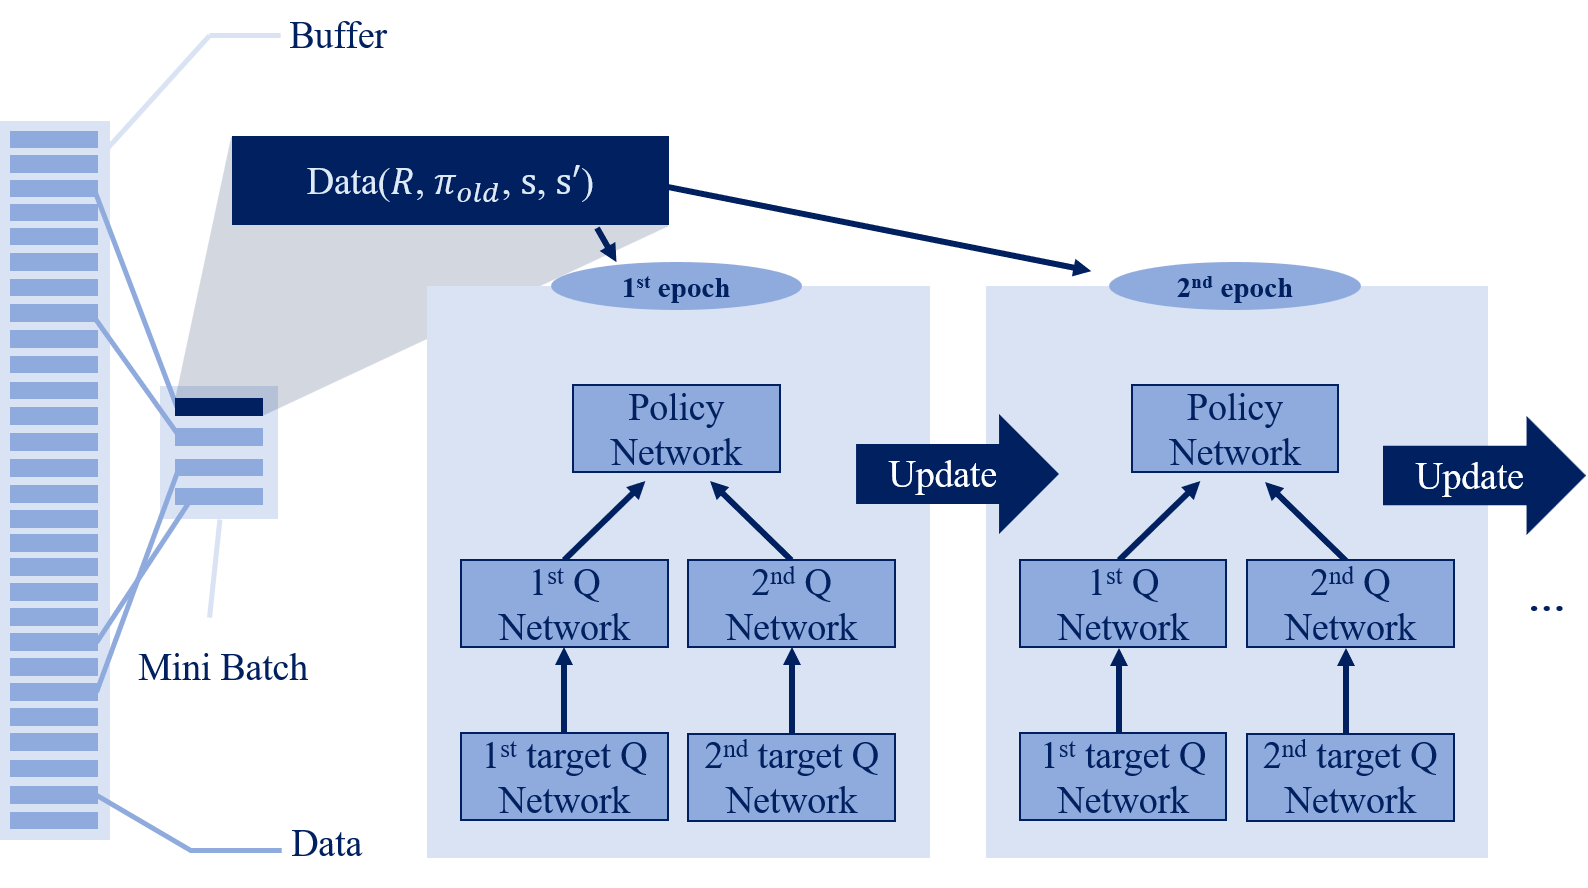
\includegraphics[width=0.8\textwidth]{./figures/sac.png}
    \caption{The SAC model in an RSU, illustrating the integration of a policy network with twin Q-networks and their target networks for dynamically selecting precaching vehicles and determining optimal content sizes.}
    \label{fig:sac}
\end{figure}

\subsection{Scenario overview} \label{sec.ov}

Our proposed framework operates in a series of distinct stages that collectively facilitate efficient content delivery in CIoV environments, as illustrated in Figure~\ref{fig:ov}: (A) A vehicle requests content, and precaching vehicles are selected and precaches the content; (B) Within the outage zone, precaching vehicles deliver its precached content to the requester vehicle; (C) When the requester vehicle enters into the subsequent RSU's communication coverage, the RSU receives the result tuple and forwards it to the previous RSU.

When a vehicle requires content, it initiates the process by sending an interest packet to the nearest~RSU.
This packet contains critical information, including the content name, the vehicle’s current location, speed, trajectory, and the identifier of the last received content chunk.
This request triggers the subsequent stages of content retrieval and precaching.
Upon receiving the request, the~RSU uses our SAC-based model to predict the optimal precaching decision.
The model processes the current state that comprises factors such as vehicle mobility, RSU coverage, and candidate vehicle information and outputs a stochastic policy that determines which candidate vehicles should precache the content and in what amount.
This prediction is crucial for adapting to dynamic and uncertain~CIoV~environments.

Based on the predicted action, the~RSU dispatches precaching instructions to the selected vehicles, specifying the exact size of the content to be cached.
The chosen precaching vehicles begin caching the designated content while still within the RSU’s coverage area.
If no suitable candidates are available, the system assigns a penalty to discourage inefficient caching.

Once the requester vehicle moves through the network and encounters either an RSU or a precaching vehicle within its communication range, the precached content is delivered to the requester vehicle.
This handoff ensures that the content is provided without incurring additional delays from fetching data from distant servers.
The success of each delivery, along with the amount of content delivered, is recorded for performance~evaluation.

Throughout this process, each experience tuple $(s, a, r, s')$ is stored in a replay buffer.
Once the buffer is full, data is randomly sampled to update the SAC model.
This off-policy learning approach leverages past experiences to enhance sample efficiency and allows the model to continuously adapt to new network conditions.
As older data is replaced by new experiences over time, the model refines its predictions, improving decision-making for both precaching vehicle selection and content size optimization.
\begin{figure}[H]
    \centering
    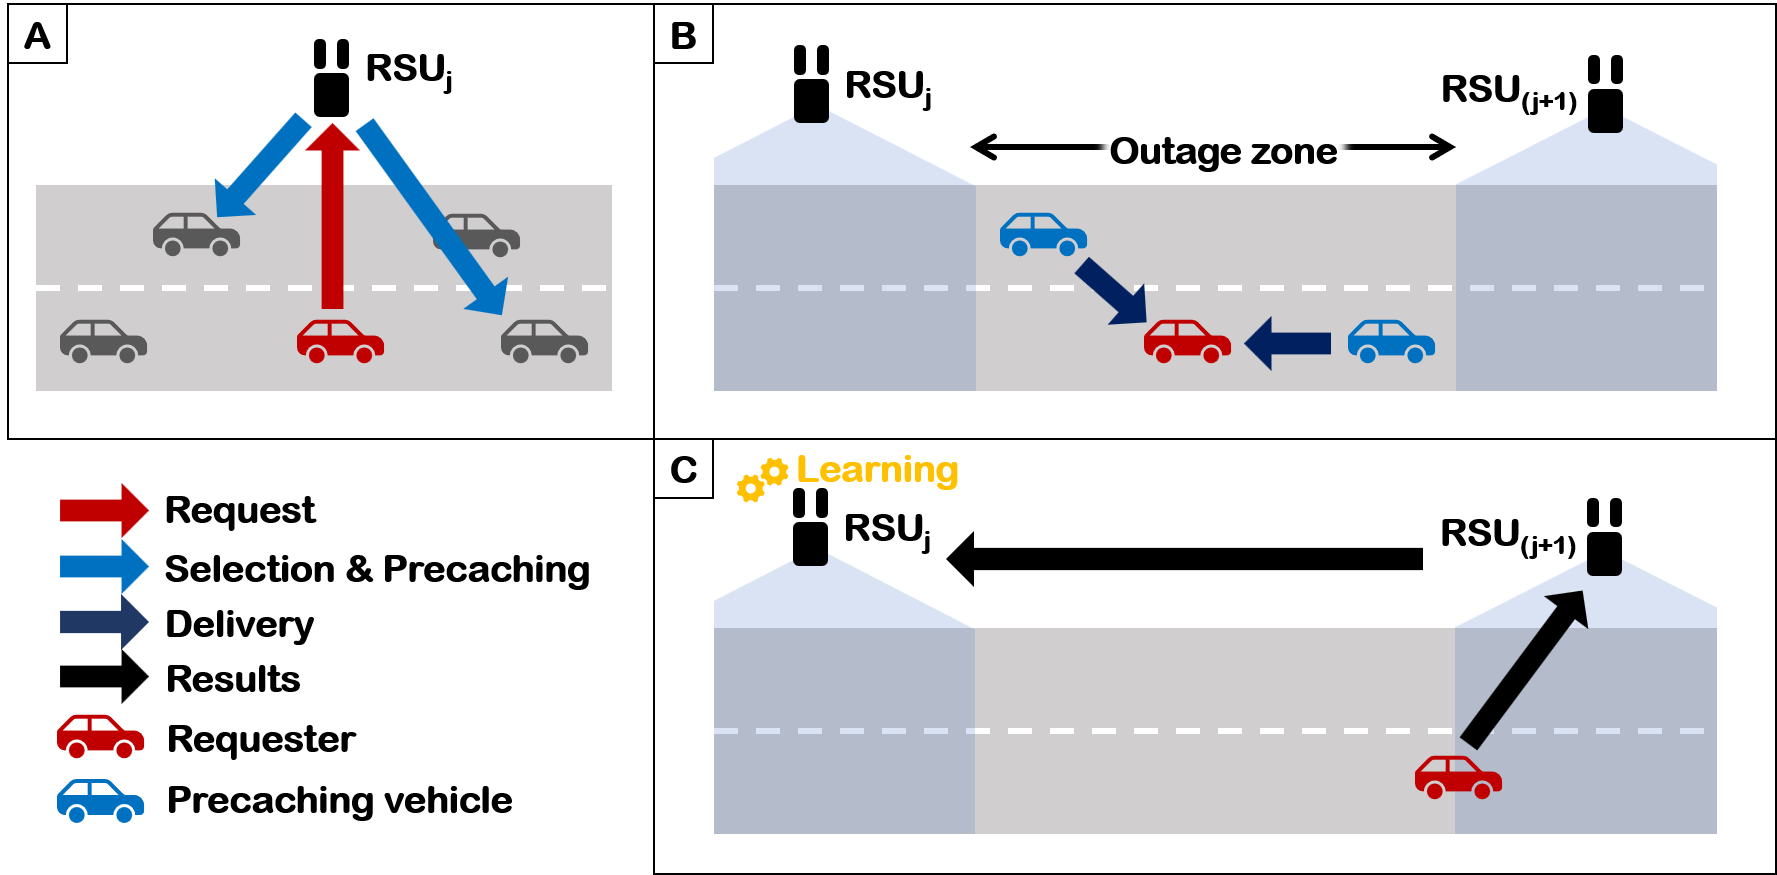
\includegraphics[width=0.8\textwidth]{./figures/overview2.png}
    \caption{An overview of the proposed SAC-based V2V precaching scheme, outlining the process from content request to delivery through continuous learning: (A) Content request and precaching vehicle selection; (B) precached content delivery within the outage zone; (C) selection result forwarding and learning.}
    \label{fig:ov}
\end{figure}
\section{SAC-based precaching vehicle selection (SAC--PVS)} \label{sec.prop}
\subsection{Content request to RSU}

When a vehicle wants to download its intended content, it requests the content by sending an interest packet using the CCN approach to the RSU where it is currently connected, and it is called the requester vehicle in this paper.
The interest packet includes the content name, the last received chunk number, the vehicle's ID, position, velocity, and trajectory, as shown in Figure \ref{fig:1}.
Based on the content name, the RSU can retrieve information about the content and locate it in its content store (CS), which is a cache storage for storing previously delivered and provided content.
By knowing the total chunk number of the content, which is one of the information, the RSU can determine the requested chunk number of the remaining content by the vehicle from the total chunk number minus the received last chunk number.
If the vehicle is requesting the content for the first time, the requested chunk number equals the total chunk number, as no chunks have yet been received.
The RSU makes a state for the request based on the information included in the interest packet.
As shown in Figure \ref{fig:2}, the state includes the remaining content size, the requester vehicle's velocity and position, the average speed of vehicles within the RSU's coverage, the communication range of both the RSU and the vehicle, the distance between this RSU and the next RSU, and the candidate vehicles' position and velocity.
For a vehicle sending an interest packet for the first time, the remaining content size is initialized to zero.
\begin{figure}[H]
    \centering
    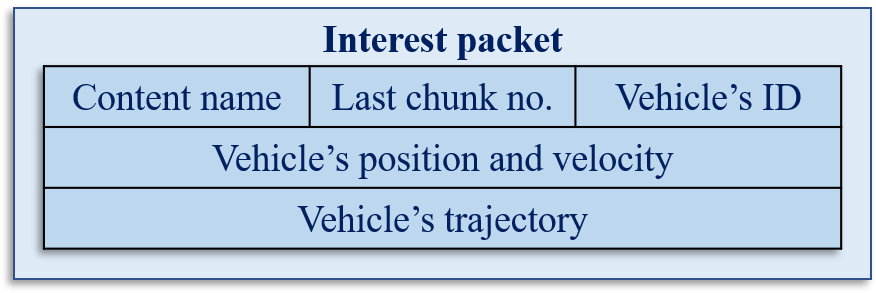
\includegraphics[width=0.45\textwidth]{./figures/2.png}
    \caption{The interest packet consisted of a content name, the last received chunk, a vehicle~ID, position, velocity, and trajectory.}
    \label{fig:1}
\end{figure}
\begin{figure}[H]
    \centering
    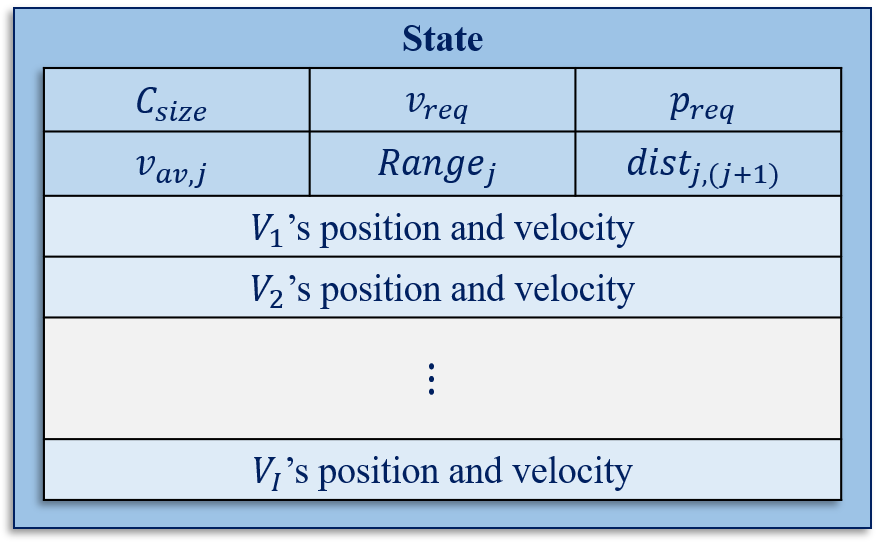
\includegraphics[width=0.45\textwidth]{./figures/3.png}
    \caption{The state for the SAC model consisted of the remaining content size, requester’s position and velocity, average speed within RSU coverage, RSU-to-RSU distance, and candidate vehicles' positions and velocities.}
    \label{fig:2}
\end{figure}
\subsection{Precaching decision prediction}


Then, according to the order of all candidate precaching vehicles, the RSU remembers their IDs.
The RSU needs to select the optimal action to choose the best precaching vehicles and determine the optimal precaching sizes based on various environmental inputs.
In this paper, we describe how the~RSU predicts these actions using the SAC algorithm.
SAC is particularly well-suited for dynamic CIoV environments due to its ability to handle continuous action spaces and maintain a balance between exploration and exploitation through entropy regularization.

SAC utilizes three neural networks: a policy (actor) network, Q-value networks (critics), and a value network.
These networks work together to maximize cumulative rewards while maintaining a high degree of exploration.

The policy network inputs the current state $s$ and outputs a stochastic policy $\pi_{\theta}(a|s)$, which provides a probability distribution over possible actions $a$.
The network is trained to maximize the expected reward while maintaining high entropy for $\pi_{\theta}(a|s)$, encouraging sustained exploration and avoiding premature convergence.
Unlike deterministic methods, SAC selects actions stochastically, which helps the RSU explore diverse strategies for precaching.
The policy network minimizes the following loss function:
\begin{equation}
    L_{\text{policy}} = \mathbb{E}_{s \sim D} \left[ \alpha \cdot \mathcal{H}(\pi_{\theta}(\cdot|s)) - Q(s, a) \right],
\end{equation}
where $\alpha$ is the entropy coefficient, $\mathcal{H}(\pi_{\theta}(\cdot|s))$ represents the entropy of the policy, and $Q(s, a)$ is the~Q-value of the state-action pair.

The Q-value networks evaluate the expected cumulative reward for each state-action pair.
Given the policy's action $a \sim \pi_{\theta}(a|s)$, the Q-value networks are updated by minimizing the Bellman error:
\begin{equation}
    L_{\text{critic}} = \mathbb{E}_{(s, a, r, s')} \left[ \big( Q(s, a) - (r + \gamma V(s')) \big)^2 \right],
\end{equation}
where $r$ is the immediate reward, $\gamma$ is the discount factor, and $V(s')$ is the value of the next state.

The value network predicts $V(s)$, which is the expected return from a state under the current policy.
It is used to stabilize the Q-value learning by acting as a baseline.
The value network minimizes the following loss function:
\begin{equation}
    L_{\text{value}} = \mathbb{E}_{s \sim D} \left[ \big( V(s) - Q(s, a) + \alpha \cdot \mathcal{H}(\pi_{\theta}(\cdot|s)) \big)^2 \right].
\end{equation}

Upon observing the current state $s$, the RSU feeds this state into the policy network to generate an action $a$, which consists of the selected precaching vehicles and their respective precaching sizes.
This action is stochastically chosen to maintain high exploration during learning.
The selected action is then executed, and the resulting reward $r$ and the next state $s'$ are used to update the Q-value and value networks.
The policy network is updated to maximize the entropy-regularized objective, ensuring a balance between exploration and exploitation.
Through this iterative process, SAC enables the RSU to learn an efficient strategy for selecting the best precaching vehicles and determining optimal precaching content sizes.


The action consists of the precaching decision value and the precaching size for each precaching candidate vehicle, as shown in Figure \ref{fig:3}.
The precaching decision value is $1$ when a candidate vehicle is selected as a precaching vehicle and $0$ otherwise.
The precaching size represents the amount of content that the RSU instructs a precaching vehicle to store.
By leveraging SAC's advanced policy optimization and entropy regularization, the RSU achieves stable and efficient action predictions across a wide range of dynamic states.


\begin{figure}[H]
    \centering
    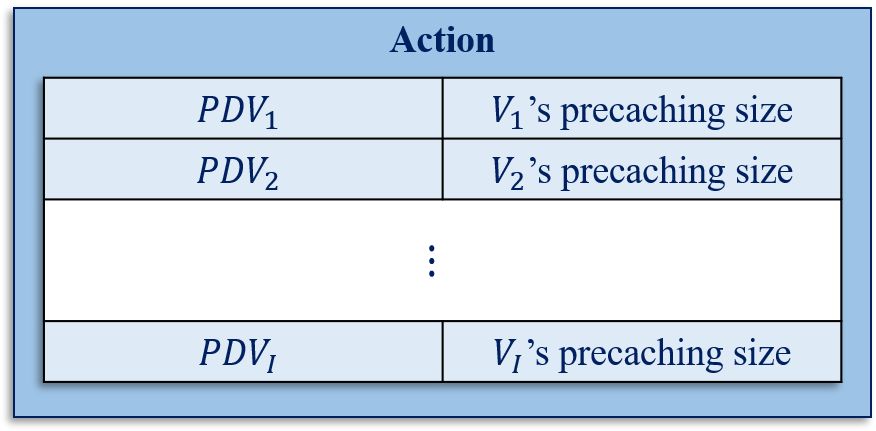
\includegraphics[width=0.45\textwidth]{./figures/4.png}
    \caption{The action vector produced by the SAC model, which encodes both the precaching decision and the content size allocation for each candidate vehicle.}
    \label{fig:3}
\end{figure}

\subsection{Precaching execution}
Based on the action predicted by the SAC algorithm, the RSU instructs the selected precaching vehicles to cache the specified content size.
If there are no candidate vehicles within the~RSU's coverage area, the SAC policy network predicts all precaching action values as zero, indicating that no precaching is necessary.
Similarly, if the RSU predicts that the requester vehicle can download the remaining content entirely within the RSU's coverage area, the action will also have zero values for the precaching decision.

In all other cases, the RSU examines the predicted action and the candidate vehicles' ordered IDs stored in memory to identify the selected precaching vehicles.
The RSU then sends a precaching packet to each selected vehicle to instruct it to precache the specified content size.
The precaching packet includes the selected vehicle's ID, the requester vehicle's ID, the content name, and the precaching size, as shown in Figure \ref{fig:4}.
Upon receiving this packet a precaching vehicle begins caching the designated content while moving within the RSU's coverage area.
However, the actual precached size may differ from the assigned size if the vehicle leaves the~RSU's coverage area early.
This discrepancy is recorded during training by storing both the assigned precaching size and the actual precached size corresponding to the vehicle's dwell time within the RSU's coverage area.

\begin{figure}[H]
    \centering
    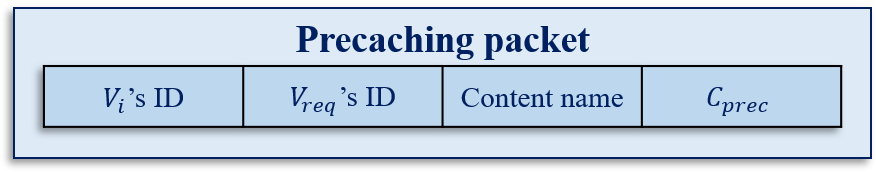
\includegraphics[width=0.45\textwidth]{./figures/5.png}
    \caption{The precaching packet consisted of a precaching vehicle's ID, the requester vehicle's ID, the content name, and the precaching size.}
    \label{fig:4}
\end{figure}

When the requester vehicle or its assigned precaching vehicle exits the RSU's communication range, the precaching vehicle becomes responsible for delivering the precached content to the requester vehicle.
Using the requester vehicle's ID from the precaching packet, the precaching vehicle identifies the requester vehicle among all vehicles within its communication range in the outage zone.
Once the requester vehicle enters its range, the precaching vehicle delivers the precached content.

For SAC-based learning, the requester vehicle tracks the total amount of content received from all assigned precaching vehicles until it reaches the next RSU's communication range.
This information, along with the observed state transitions, is used by the SAC algorithm to refine the policy and Q-value networks for optimizing future actions.
Additionally, when a precaching vehicle enters the next RSU's communication range, it resets its stored requester vehicle ID to prepare for new tasks.

Upon entering into the coverage area of the next RSU ($R_{j+1}$), the requester vehicle sends an interest packet to $R_{j+1}$.
If the last chunk number in this packet is not zero, indicating incomplete content delivery, $R_{j+1}$ sends a result packet back to the previous RSU ($R_{j}$).
The result packet includes the requester vehicle's ID, the actual delivered content size, and the new state $s'$, as shown in Figure \ref{fig:5}.
This feedback mechanism allows the SAC algorithm to adjust its policy and Q-value networks for improving its decision-making in future iterations.
\newpage
\begin{figure}[H]
    \centering
    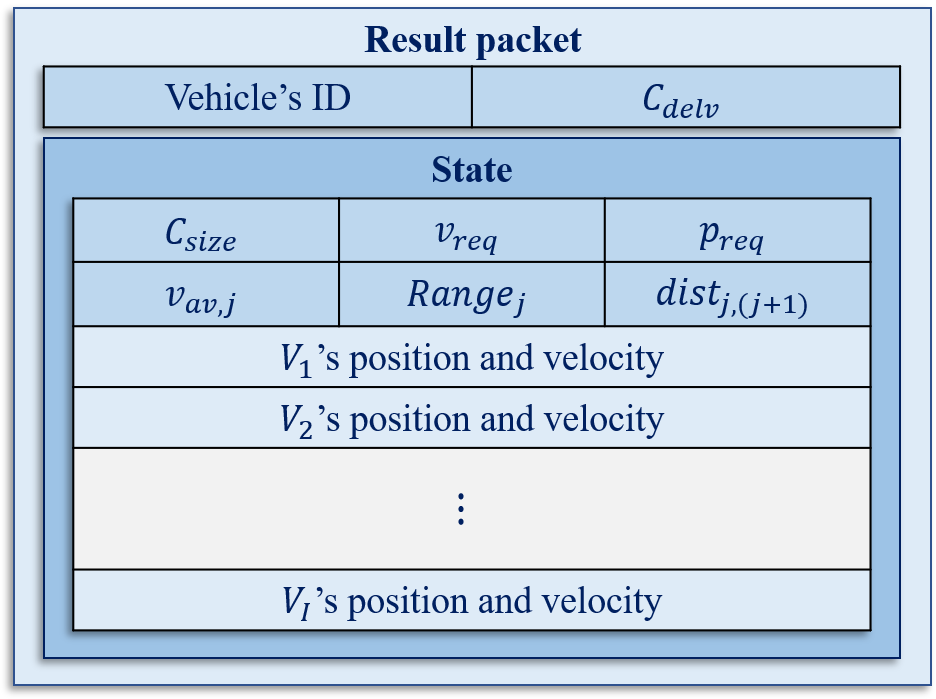
\includegraphics[width=0.45\textwidth]{./figures/6.png}
    \caption{The result packet from the next RSU consisted of the requester vehicle’s ID, the delivered content size, and the updated state used to refine the model’s learning.}
    \label{fig:5}
\end{figure}


\subsection{Precaching delivery and feedback}
Upon receiving the result packet from $R_{j+1}$, $R_{j}$ updates its stored information data for the requester vehicle, including the current state $s$, the predicted action $\pi_{\theta}(a|s)$, the reward $r_{stg}$, and the next state~$s'$.
These updated tuples $(s, \pi_{\theta}(a|s), r_{stg}, s')$ are then appended to a replay buffer.
Once the buffer accumulates a sufficient number of samples (i.e., reaching the preset buffer size), our SAC model initiates training.
During this phase, the model randomly samples mini-batches from the buffer to perform off-policy learning.
It reuses past experiences efficiently.
After each training cycle, new samples replace the oldest ones, ensuring that the buffer remains up-to-date with the latest network~dynamics.

Our reward function is designed in two stages and is applied consistently to both the precaching vehicle selection model and the precaching quantity decision model.
In the first stage, the precaching vehicle selection model identifies which vehicles should cache the requested content.
In this stage, the model receives a state $s$ and, through the policy $\pi_{\theta}(a|s)$, produces an action $a$ that determines which candidate vehicles will be chosen.
Based on this predicted action, $R_{j}$ selects the appropriate vehicles for precaching.
Subsequently, the precaching quantity decision model determines how much content each selected vehicle should cache.
This model incorporates the selection information from the previous stage as part of the state $s$.
Using this enriched state, $R_{j}$ then decides the precise amount of content that each selected vehicle needs to precache.
By integrating both stages under a unified reward function, our two models not only optimize the vehicle selection process but also fine-tune the content allocation, ultimately enhancing the overall efficiency of content delivery in dynamic CIoV environments.

\textbf{Stage 1 (Selection reward):}
This reward penalizes inefficient candidate selection.
The size of the candidate space $N_{s}$ is defined by
\begin{equation}
    N_{s}= N_{dir} \times Dens_{max},
\end{equation}
where $N_{dir}$ indicates 4 directions (front, back, left, right) in an RSU's communication coverage and $Dens_{max}$ is the maximum number of vehicles per 1 km lane.
Using $N_{s}$, the selection reward is computed as follows:
\begin{equation}
\begin{split}
    r_{1} &= N_{s} \delta_{fill} - \delta_{empt}\cfrac{N_{s}}{2}
            + 2N_{s} \cfrac{\delta_{fill}}{N_{s}} - \gamma_{p} N_{s} \delta_{n}\\
          &= \left(N_{s}+2\right)\delta_{fill}-N_{s}\left(\cfrac{\delta_{empt}}{2}+\gamma_{p}\delta_{n}\right).
\end{split}
\end{equation}
Candidate vehicles are sequentially entered into a fixed state space, resulting in areas that are filled with candidate information and areas that remain empty.
Here, $\delta_{fill}$ denotes the number of vehicles selected from the portions where candidate information is filled, while $\delta_{empt}$ represents the number of vehicles chosen from the unfilled portions.
In addition, $\delta_{n}$ is an indicator that is set to 1 when there existed candidate spaces, but no one is selected.
$N_{s} \delta_{fill}$ is the reward for the successful selection.
$\delta_{empt}N_{s}/2$ is the penalty for the wrong selection.
To enhance the reward, we set an additional reward of $2N_{s} (\delta_{fill}/N_{s})$ that denotes the ratio of the successful selection.
To give a strong penalty for not selecting any candidate when available, we set $\gamma_{p} N_{s} \delta_{n}$ where the reflection intensity $\gamma_{p}$ is 3.

\textbf{Stage 2 (Precaching reward):}
This stage evaluates the content delivery performance by considering the actual delivery and penalizing poor choices.
The precaching reward is computed as~follows:
\begin{equation}
    r_{2} = S_{d} - \cfrac{N_{s}\delta_{wrong}}{2}-\gamma_{p}N_{s}\delta_{n},
\end{equation}
where $S_{d}$ is the total amount of content successfully delivered to the requester and $\delta_{wrong}$ is the number of wrong selections (i.e., when the selected precaching vehicle fails to deliver the precached content).

This hierarchical training approach enables our model to effectively learn both the optimal vehicle selection strategy and the precise allocation of precaching sizes, ensuring efficient and reliable content delivery to requester vehicles in outage zones.
By structuring the learning process in progressive stages, the model achieves greater stability, faster convergence, and improved adaptability to dynamic vehicular environments.
This approach minimizes wasted traffic, enhances the utilization of network resources, and ultimately improves the overall Quality of Experience (QoE) for CIoV users.

\subsection{SAC model training with request data}
As shown in Figure \ref{fig:sac}, the SAC model in each RSU updates its policy, Q-value, and target Q-value neural networks to optimize precaching decisions.
The RSU collects experience data $(s, a, r, s')$ from multiple requester vehicles and stores them in a replay buffer.
The SAC algorithm samples mini-batches of data from the replay buffer to perform training, ensuring that the agent learns from a diverse set of past experiences.

SAC aims to maximize the expected reward while encouraging exploration through entropy regularization.
The objective function for the policy neural network of SAC is given as:
\begin{equation}
    J_{\pi}(\phi) = \mathbb{E}_{s \sim \mathcal{D}} \left[ \alpha \mathcal{H}(\pi_{\phi}(\cdot|s)) + Q_{\theta}(s, a) \right],
\end{equation}
where $\mathcal{H}(\pi_{\phi}(\cdot|s))$ represents the entropy of the policy $\pi_{\phi}(a|s)$, which encourages exploration by maximizing randomness in the action selection process.
$\alpha$ is the temperature parameter that controls the trade-off between exploration (via entropy) and exploitation (via expected reward).

The Q-value neural network is trained using the following loss function:
\begin{equation}
    \begin{split}
        J_Q(\theta) = & \mathbb{E}_{(s, a, r, s') \sim \mathcal{D}} \left[ \left( Q_{\theta}(s, a) - \left( r \right.\right.\right.\\
        & \left.\left.\left.+ \gamma \mathbb{E}_{a' \sim \pi_{\phi}(s')} [Q_{\theta'}(s', a') - \alpha \log \pi_{\phi}(a'|s')] \right) \right)^2 \right],
    \end{split}
\end{equation}
where $Q_{\theta}(s, a)$ is the Q-value estimated by the current Q-network, $Q_{\theta'}(s', a')$ is the target Q-value, and~$\gamma$ is the discount factor.

The policy network $\pi_{\phi}$ and the Q-value network $Q_{\theta}$ are updated iteratively during training.
The target Q-value network is updated less frequently to stabilize training, as follows:
\begin{equation}
    \theta' \leftarrow \tau \theta + (1 - \tau) \theta',
\end{equation}
where $\tau$ is the soft update rate.

Entropy regularization in the SAC enables the RSU to effectively balance exploration and exploitation, making it robust to the dynamic nature of CIoV.
Through continuous sampling and learning from the replay buffer, SAC learns optimal precaching decisions that minimize latency and maximize content delivery efficiency within outage zones in CIoV.


\section{Performance evaluation} \label{sec.perf}

\subsection{Simulation environment} \label{sec.s1}
In this section, we evaluate the performance of the proposed SAC-PVS scheme through simulations in a grid-based Manhattan mobility scenario.
Our reinforcement learning framework is implemented using the Stable Baselines3 library in Python, and then compare our approach to other baseline methods \cite{SB3}.
A 10km $\times$ 10km urban region is configured in a grid-shaped Manhattan model to emulate a city-like environment.
Each intersection hosts a single RSU, resulting in a uniform deployment of RSU at all junctions.
The RSUs are interconnected via high-speed fiber links, featuring a transmission rate of 10Gbps and a latency of 10ms, enabling efficient content exchange with the content server and among RSUs.
Each RSU can cache up to 1TB of content, and provides services to vehicles through WAVE communication.

Vehicles traverse the Manhattan grid following the shortest-path routes toward randomly assigned destinations.
To approximate realistic driving conditions while maintaining computational tractability, each vehicle’s speed is sampled from a Gaussian distribution with skewness, reflecting variations in acceleration and deceleration.
Vehicles communicate with RSUs via WAVE whenever they are within coverage.
In outage zones with insufficient RSU coverage, vehicles can engage in V2V precaching and content forwarding via WAVE, enabling them to share cached content with nearby vehicles.
Vehicle periodically requests content from RSUs according to a Poisson process, with an average interval between requests of 15 seconds, except when the content is already being downloaded.
Content popularity follows a Zipf distribution~(exponent~0.75) from a pool of 1,000,000 items. Each piece of content is subdivided into chunks of~25kB.
Vehicles can locally cache up to 256GB of data, and when operating in outage zones, they may rely on~V2V connections to access or relay precached content.

We implement our SAC-based learning framework using Stable Baselines3 in Python.
Each vehicle’s experience $(s, a, r, s')$ is stored in a replay buffer until it reaches a preset capacity, after which mini-batches are sampled for off-policy training.
Older samples are removed in a FIFO manner as new data arrives.
The key SAC hyperparameters, such as buffer size, discount factor $\gamma$, and learning rate, are detailed in Table~\ref{table1}.
The entropy coefficient $\alpha$ is automatically tuned by stable baselines3.
We run the simulation for a total of 72,000s (20h of simulated time) to capture diverse traffic patterns and mobility events.
Each experiment is repeated for 10,000 iterations to ensure statistical significance.
Performance metrics, including content download delay and wasted link traffic, are compared across baseline methods, including~PPO-based approaches and none-ML precaching strategies.

\begin{table}[H] % table1
    \caption{Simulation parameters.}
    \centering
    \begin{tabular}{cc}
        \hline
        \textbf{Parameters} & \textbf{Value} \\
        \hline
        Simulation time & 7200 s\\
        Network size & 10 km $\times$ 10 km\\
        Distance between RSUs & 1 km\\
        Vehicle mobility model & Manhattan case \\
        
        Backhaul link latency & 10 ms\\
        Backhaul link rate & 10 Gbps\\
        Maximum $r_{j}(t)$ & 54 Mbps\\
        
        An exponent of content popularity & 0.75\\
        Chunk size & 25 kbytes\\
        
        RSU transmission range & 800 m\\
        
        Vehicle's CS & 256 GB\\
        RSU's CS & 1 TB\\

        Vehicle density & [2, 20] per {km}$^{2}$\\
        Vehicles' average speed & [20, 60] km/h\\
        Content request mean $\lambda$ & 15 s\\
        Size of requested content & [1000,3000] MB \\

        Buffer size & 10$^{5}$ \\
        Learning Rate & 10$^{-4}$ \\
        Discount Factor $\gamma$ & 0.99 \\
        Soft Update Coefficient $\tau$ & 0.005 \\
        Entropy Coefficient $\alpha$ & auto \\
        train freq & 1 \\
        gradient steps & 1 \\
        \hline
    \end{tabular}
    \label{table1}
\end{table}

For the X-axis, we consider three key variables: vehicle speed, vehicle density, and requested content size, as follows:
\begin{itemize}
    \item \textbf{Vehicle speed:} It denotes the average rate at which vehicles travel within the network, impacting the duration of RSU connectivity and delays.
    \item \textbf{Vehicle density:} It quantifies the number of vehicles per unit area.
    Higher density increases overall connectivity and the pool of candidate precaching vehicles,  improving the selection~process.
    \item \textbf{Requested content size:} It reflects the volume of content that vehicles request, with larger sizes leading to longer download times and placing greater demands on caching resources.
\end{itemize}

For the Y-axis, our evaluation focuses on the total content download time and the wasted traffic as~follows:
\begin{itemize}
    \item \textbf{Rewards:} We quantify the performance of our precaching strategy in two stages.
    In Stage 1, rewards are calculated based on the accurate selection of candidate vehicles, while penalties are applied for empty or missed selections—reflecting the model’s effectiveness in choosing appropriate precaching vehicles.
    In Stage 2, rewards are determined by the amount of successfully delivered content, with penalties imposed for incorrect selections that hinder content delivery.
    Together, these reward mechanisms provide a key indicator of overall system efficiency and the Quality of Experience (QoE).
    \item \textbf{The total content download time:} It captures the interval from when a vehicle initiates a request until the entire content is received, serving as an indicator of the overall efficiency of the delivery system.
    Also, it can reflect QoE performances for users.
    \item \textbf{The wasted traffic:} It measures the volume of content that is precached but ultimately not delivered, thus providing insight into the effectiveness of the caching strategy and resource~utilization.
\end{itemize}
Lower values in both metrics are desirable, as they indicate a faster, more efficient content delivery and a reduction in unnecessary network load.

To demonstrate the advantages of our proposed scheme in dynamic vehicular environments, we compare it with two baseline approaches:
1) The PPO scheme, an on-policy method that updates its policy using only fresh data from each episode while discarding previous experiences, which can limit sample efficiency and adaptability in rapidly changing conditions; and
2) the no-ML scheme \cite{Nam2023}, which relies solely on mathematical optimization to predict vehicle mobility and make precaching decisions.
While computationally efficient, static models often fail to capture the complex, real-time variations inherent in vehicular networks.
In contrast, our SAC-based scheme leverages off-policy learning to reuse past experiences via a replay buffer.
It also employs entropy regularization to balance exploration and exploitation effectively.
This combination enables faster convergence, higher prediction accuracy, and robust performance in dynamic CIoV scenarios.


\subsection{Ablation study and sensitivity analysis} \label{sec.ablation}
To ensure the reliability and robustness of our proposed SAC-PVS scheme, we conducted a comprehensive ablation study and sensitivity analysis.
This process validates the contribution of each reward function and evaluates the impact of critical hyperparameters—specifically the Discount Factor $\gamma$, Entropy Coefficient $\alpha$, and Learning Rate—on model convergence.


\subsubsection{Ablation study}
We first verify the design of our hierarchical reward function through an ablation study.
We compare the convergence performance of the full model \textit{All} against three variants in which specific reward or penalty terms are removed.
The configurations are as follows:
\begin{itemize}
    \item \textbf{No fill reward:} This variant removes the positive reinforcement $\delta_{fill}$ granted when the agent correctly selects a vehicle in a filled candidate space.
    As shown in the results, this component is essential for accessing higher rewards.
    Without it, the agent lacks the incentive to actively explore and exploit profitable states, leading to a failure to show the performance improvement characteristic of effective learning.
    \item \textbf{No empty penalty:} This variant eliminates the penalty $\delta_{empt}$ applied when the agent incorrectly selects an empty space.
    The results suggest this penalty plays a key role in stability.
    By explicitly discouraging invalid selections, it reduces the variance in the agent's actions, leading to a more stable learning curve compared to the fluctuating performance observed when this penalty is~removed.
    \item \textbf{No selection penalty:} This variant discards the penalty $\delta_{n}$ imposed when the agent selects nothing despite available candidates.
    We infer that this component serves as an activation signal to prevent active laziness.
    Without it, the agent tends to settle for a safe but suboptimal inaction strategy to avoid potential risks, failing to capitalize on valid precaching opportunities.
\end{itemize}



As shown in Figure \ref{fig:add1}, the proposed All scheme achieves the highest stable reward.
The No Fill Reward variant fails to rise to positive values, confirming its role in driving performance growth.
The No Empty Penalty variant exhibits less stability, while the No Selection Penalty variant converges to a lower suboptimal value, indicating passivity.
These findings confirm that the full reward function, which combines the growth drive of $\delta_{fill}$, the stabilizing force of $\delta_{empt}$, and the activation pressure of~$\delta_{n}$, is essential for maximizing precaching efficiency.
\begin{figure}[H]
    \centering
    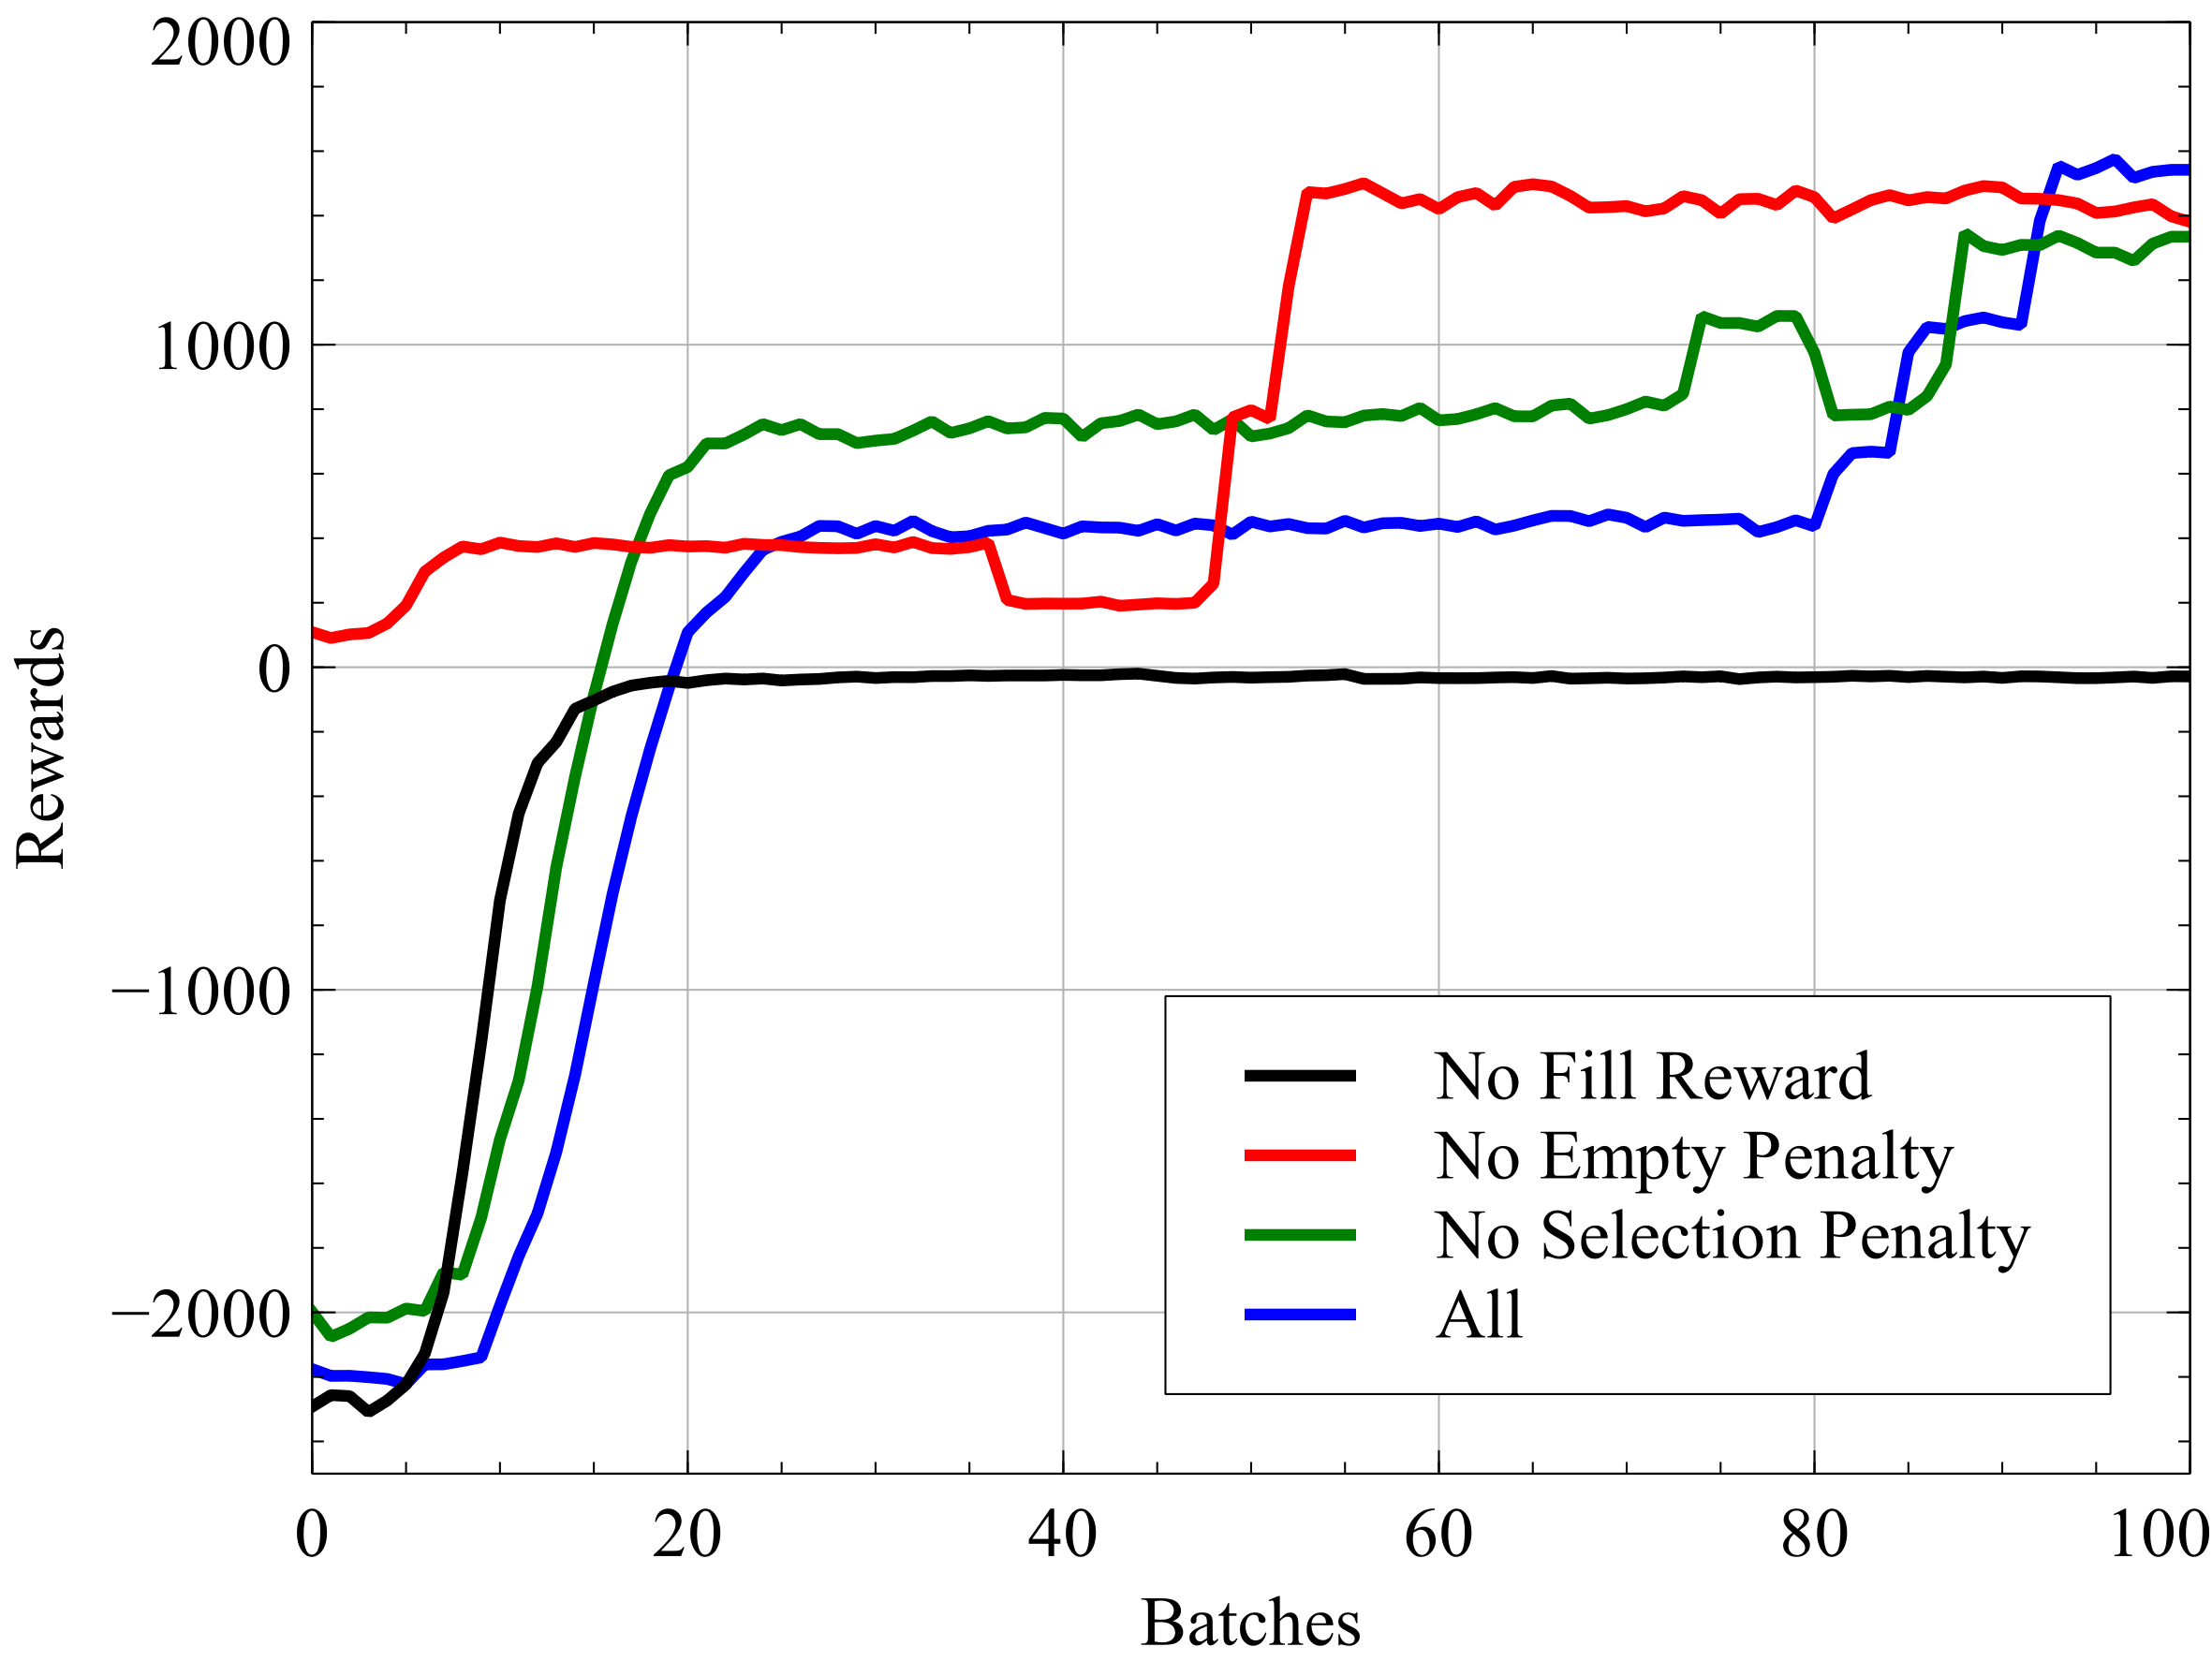
\includegraphics[width=0.55\textwidth]{./graphs/Add1.png}
    \caption{Ablation study of reward function components: comparison of convergence performance among the full model and variants removing specific reward/penalty terms.}
    \label{fig:add1}
\end{figure}
\subsubsection{Sensitivity analysis of key SAC parameters}
In SAC, the Discount Factor $\gamma$ and Entropy Coefficient $\alpha$ are the most critical hyperparameters governing the learning process.
The entropy coefficient determines the trade-off between exploration and exploitation.
In our implementation, we utilized the automatic entropy tuning mechanism, which dynamically adjusts $\alpha$ during training to maintain a target entropy based on stable baselines 3 \cite{SB3}.
Since this adaptive method consistently provides optimal exploration without manual intervention, validation results for fixed $\alpha$ values are not included in this analysis.



The discount factor is crucial for V2V precaching due to the delayed nature of rewards (i.e., content delivery occurs after traversing the outage zone).
We investigated the impact of $\gamma$ by comparing performance across different values as shown in Figure \ref{fig:add2}.
While lower discount factors such as~0.90 and 0.95 facilitated rapid initial convergence and demonstrated stable performance, they tended to stagnate at slightly lower peak rewards compared to the optimal setting.
In contrast, the model with~$\gamma = 0.99$ exhibited higher variance in the final training stages, but it achieved the highest peak reward~(approximately 1575), surpassing the maximum values obtained by other settings.
This behavior indicates that a higher discount factor encourages the agent to continuously explore and fine-tune its policy to capture the sparse and delayed rewards inherent in outage zone traversal, rather than settling for a stable but suboptimal local solution.
Therefore, despite the increased training instability, we selected $\gamma = 0.99$ to maximize the system's potential for achieving the global optimum and ensuring the highest possible quality of service.
\begin{figure}[H]
    \centering
    \includegraphics[width=0.55\textwidth]{./graphs/Add2.png}
    \caption{Discount Factor.}
    \label{fig:add2}
\end{figure}

\subsubsection{Impact of learning rate}
Finally, we examined the influence of the Learning Rate, another vital hyperparameter for training~stability.



Figure \ref{fig:g21} illustrates how different learning rates influence reward progression in Stage 1 of the precaching vehicle selection model.
Overall, each learning rate converges to a relatively high reward, but the curves reveal subtle differences in stability and convergence speed.
A higher learning rate tends to accelerate early gains but may exhibit occasional fluctuations, while a lower rate converges more steadily, potentially achieving a smoother reward profile and higher peak reward.
The intermediate rate balances these tendencies, showing moderate initial progress along with decent stability.
Comparing these three curves, one can select the most suitable learning rate based on whether faster convergence or a more stable learning trajectory is prioritized in the vehicular network environment.

Figure \ref{fig:g22} illustrates the impact of different learning rates on reward progression in Stage 2 of the precaching vehicle selection model.
The highest learning rate curve shows rapid initial improvements but experiences more pronounced fluctuations, whereas the lower rate exhibits a slower yet more stable ascent in reward.
The intermediate rate strikes a balance between these two behaviors, offering both reasonable convergence speed and steadiness.
By comparing these trajectories, one can identify which rate best suits the demands of the network environment, whether a faster but potentially less stable approach or a slower yet more reliable one is desired.

Figure \ref{fig:g23} compares the effects of different learning rates on Stage 1 of the precaching quantity decision model.
All three curves converge relatively quickly, but the highest rate exhibits a steeper initial rise followed by more noticeable oscillations, indicating rapid learning at the cost of potential instability.
In contrast the lowest learning rate, progresses more gradually and demonstrates smoother updates.
The intermediate rate falls between these extremes, balancing faster convergence with fewer fluctuations.
These trends help guide the selection of a learning rate that best aligns with the desired trade-off between learning speed and stability in precaching amount decisions.

Figure \ref{fig:g24} illustrates the impact of how different learning rates on Stage 2 of the precaching quantity decision model.
Stage 2 of the precaching quantity decision model has already been heavily trained by the previous step, so all curves converge around a positive reward value.
With sufficient training time, each rate appears capable of converging toward a similar level of performance.
Overall, the differences among these learning rates become less significant over extended training, indicating that the model can eventually converge to a comparable reward level regardless of the specific rate chosen.

\begin{figure}[H]
    \centering
    \subfigure[]{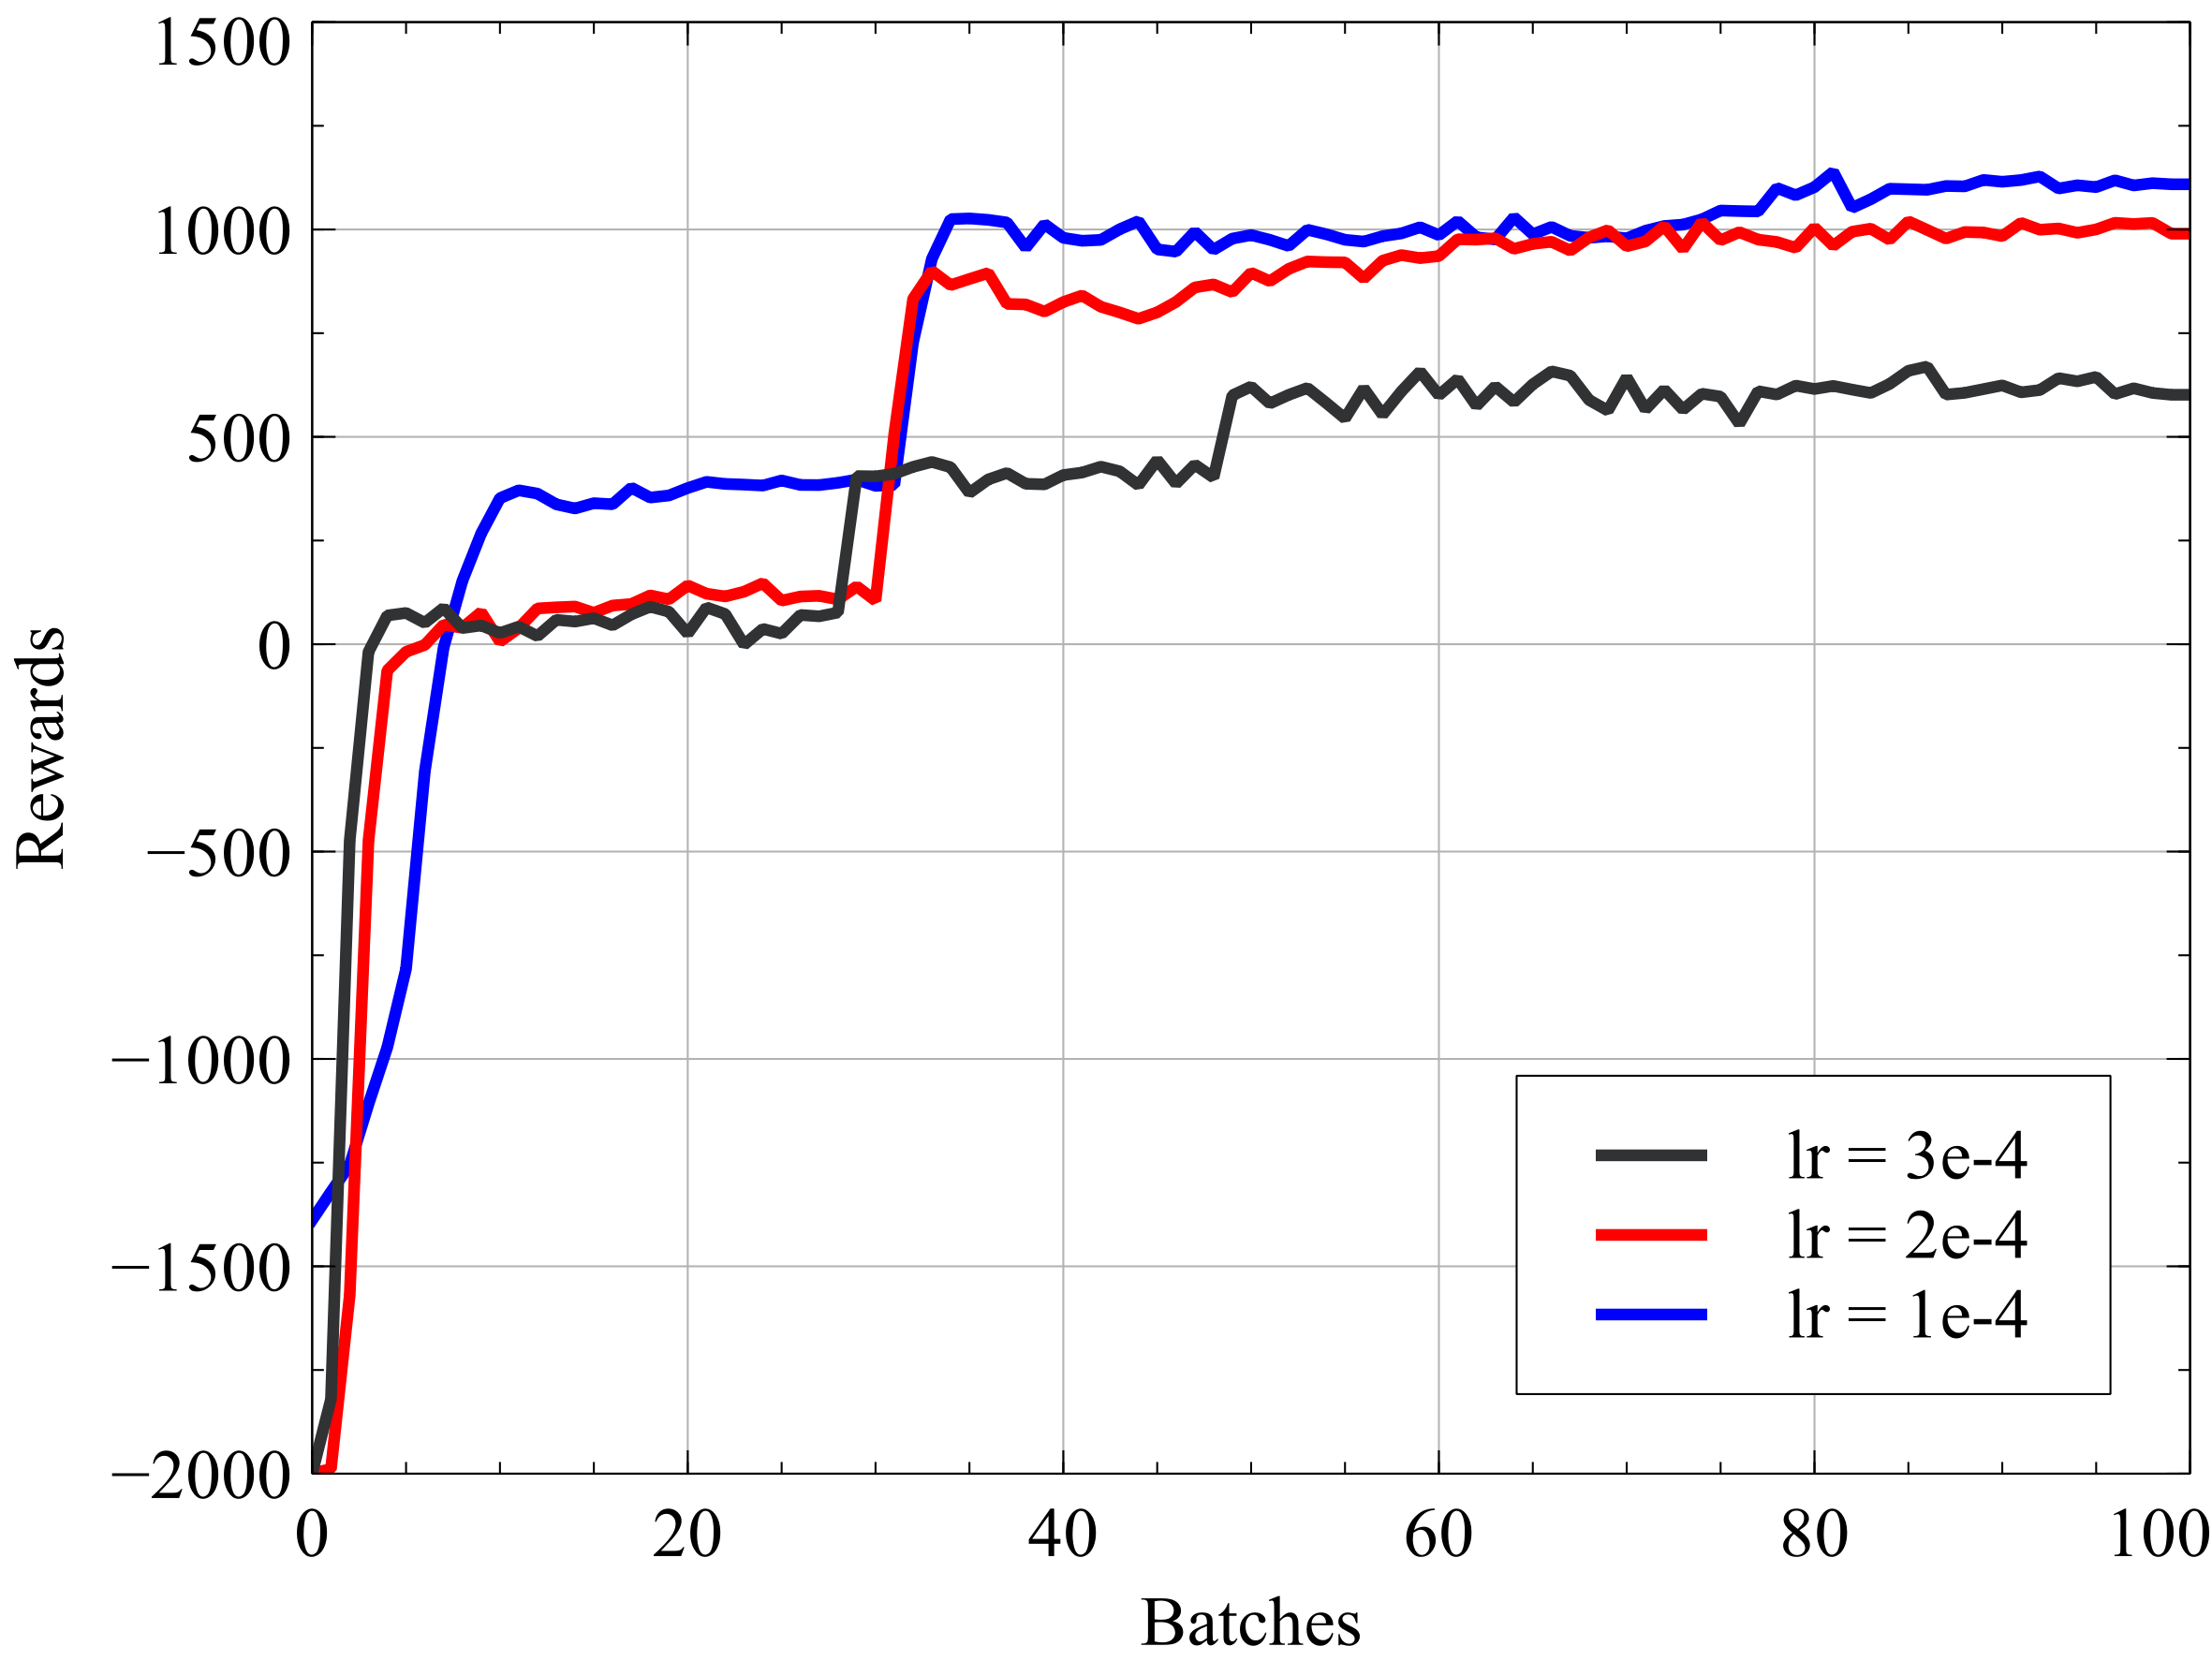
\includegraphics[width=0.42\textwidth]{./graphs/Results_03.png} \label{fig:g21}}
    \subfigure[]{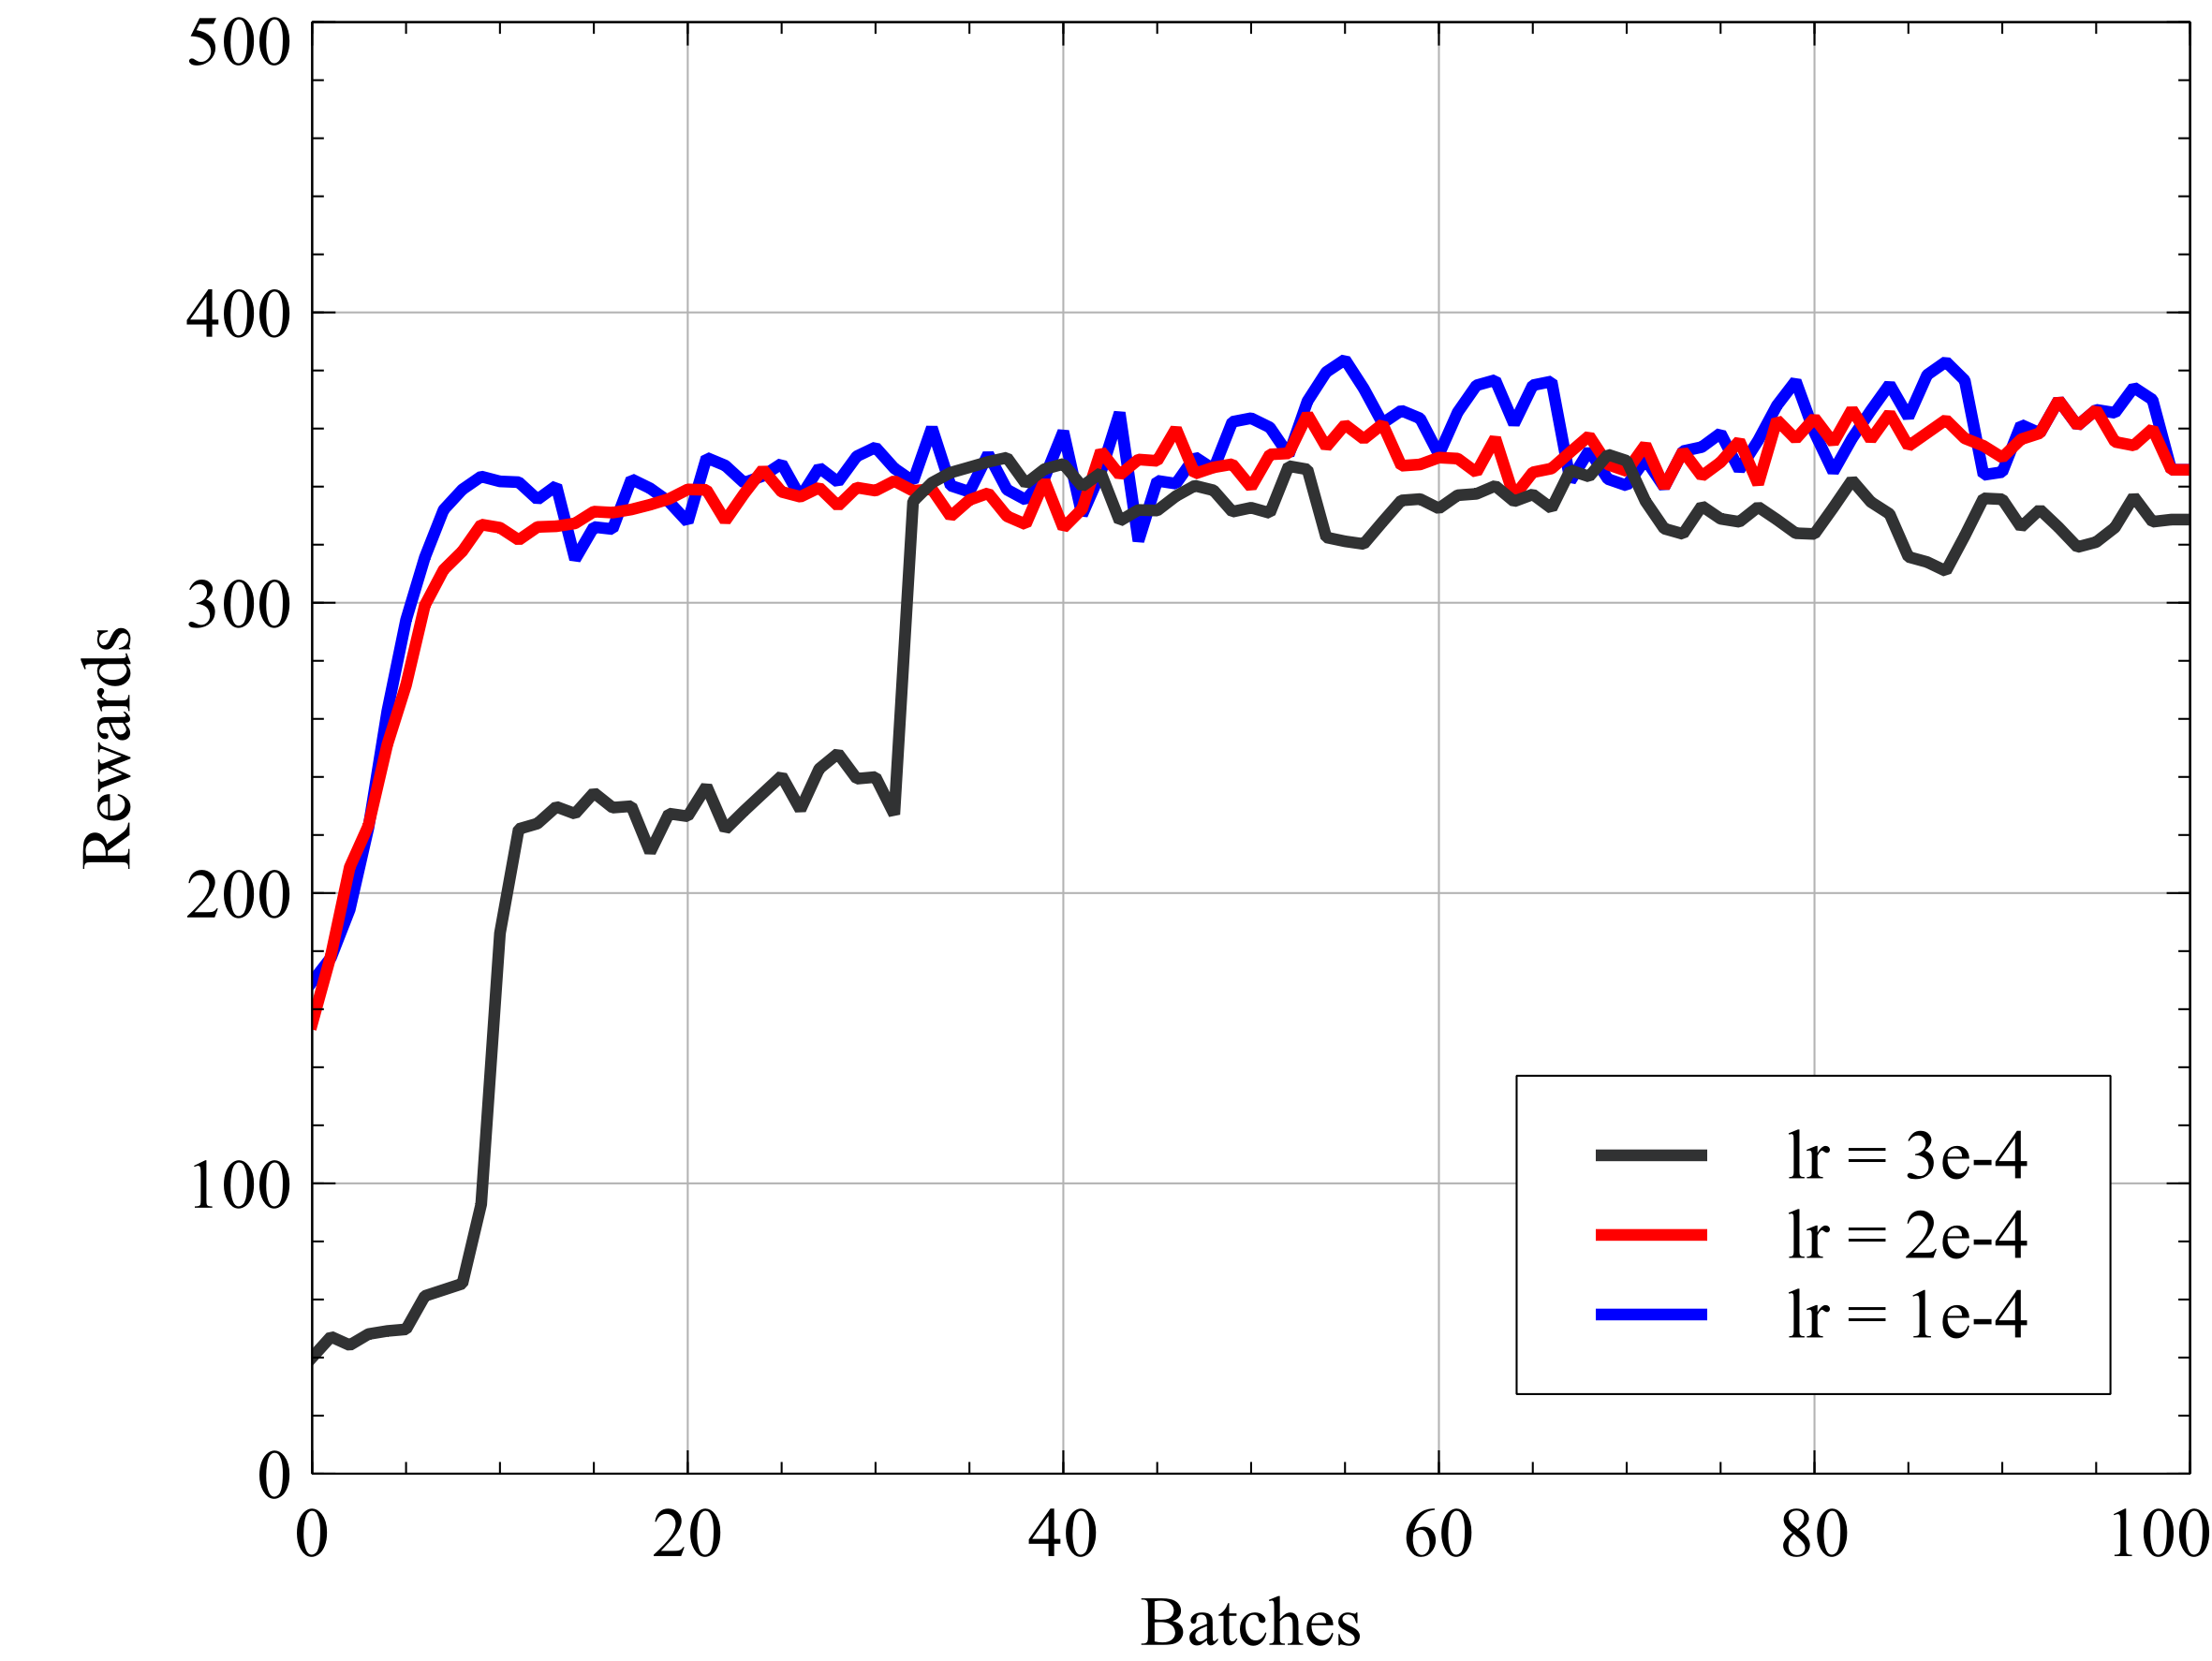
\includegraphics[width=0.42\textwidth]{./graphs/Results_04.png} \label{fig:g22}}\\
    \subfigure[]{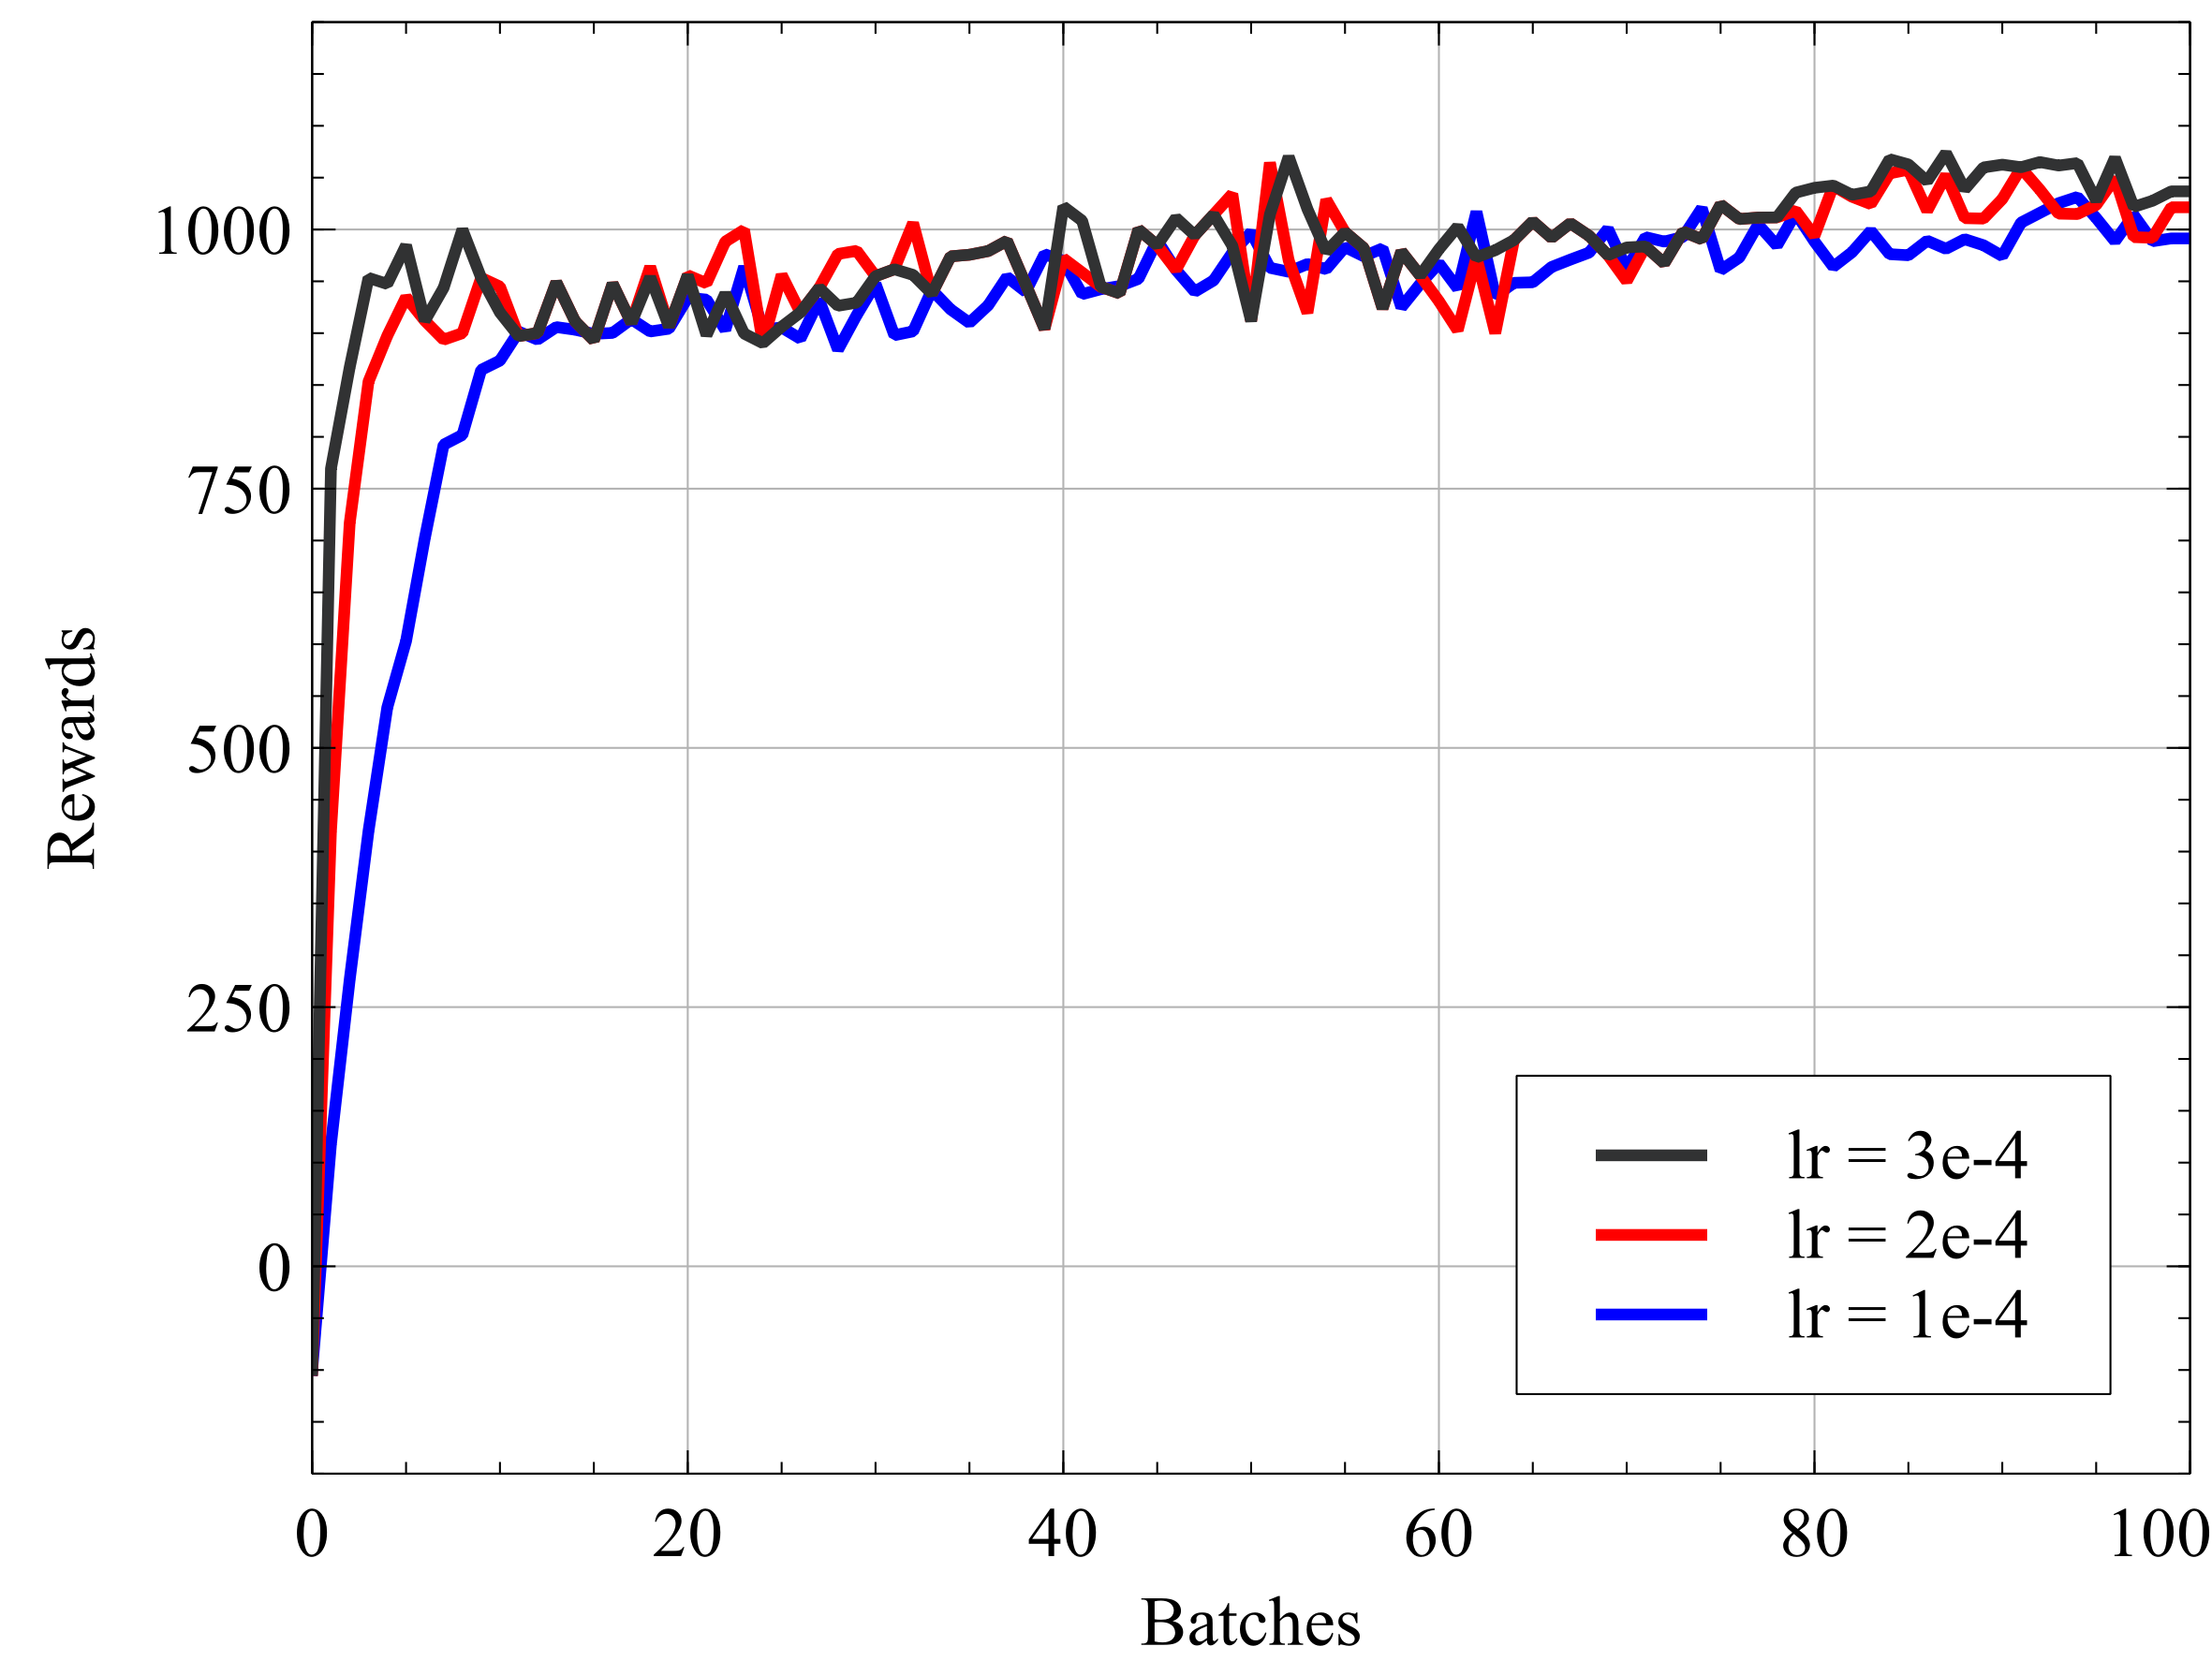
\includegraphics[width=0.42\textwidth]{./graphs/Results_07.png} \label{fig:g23}}
    \subfigure[]{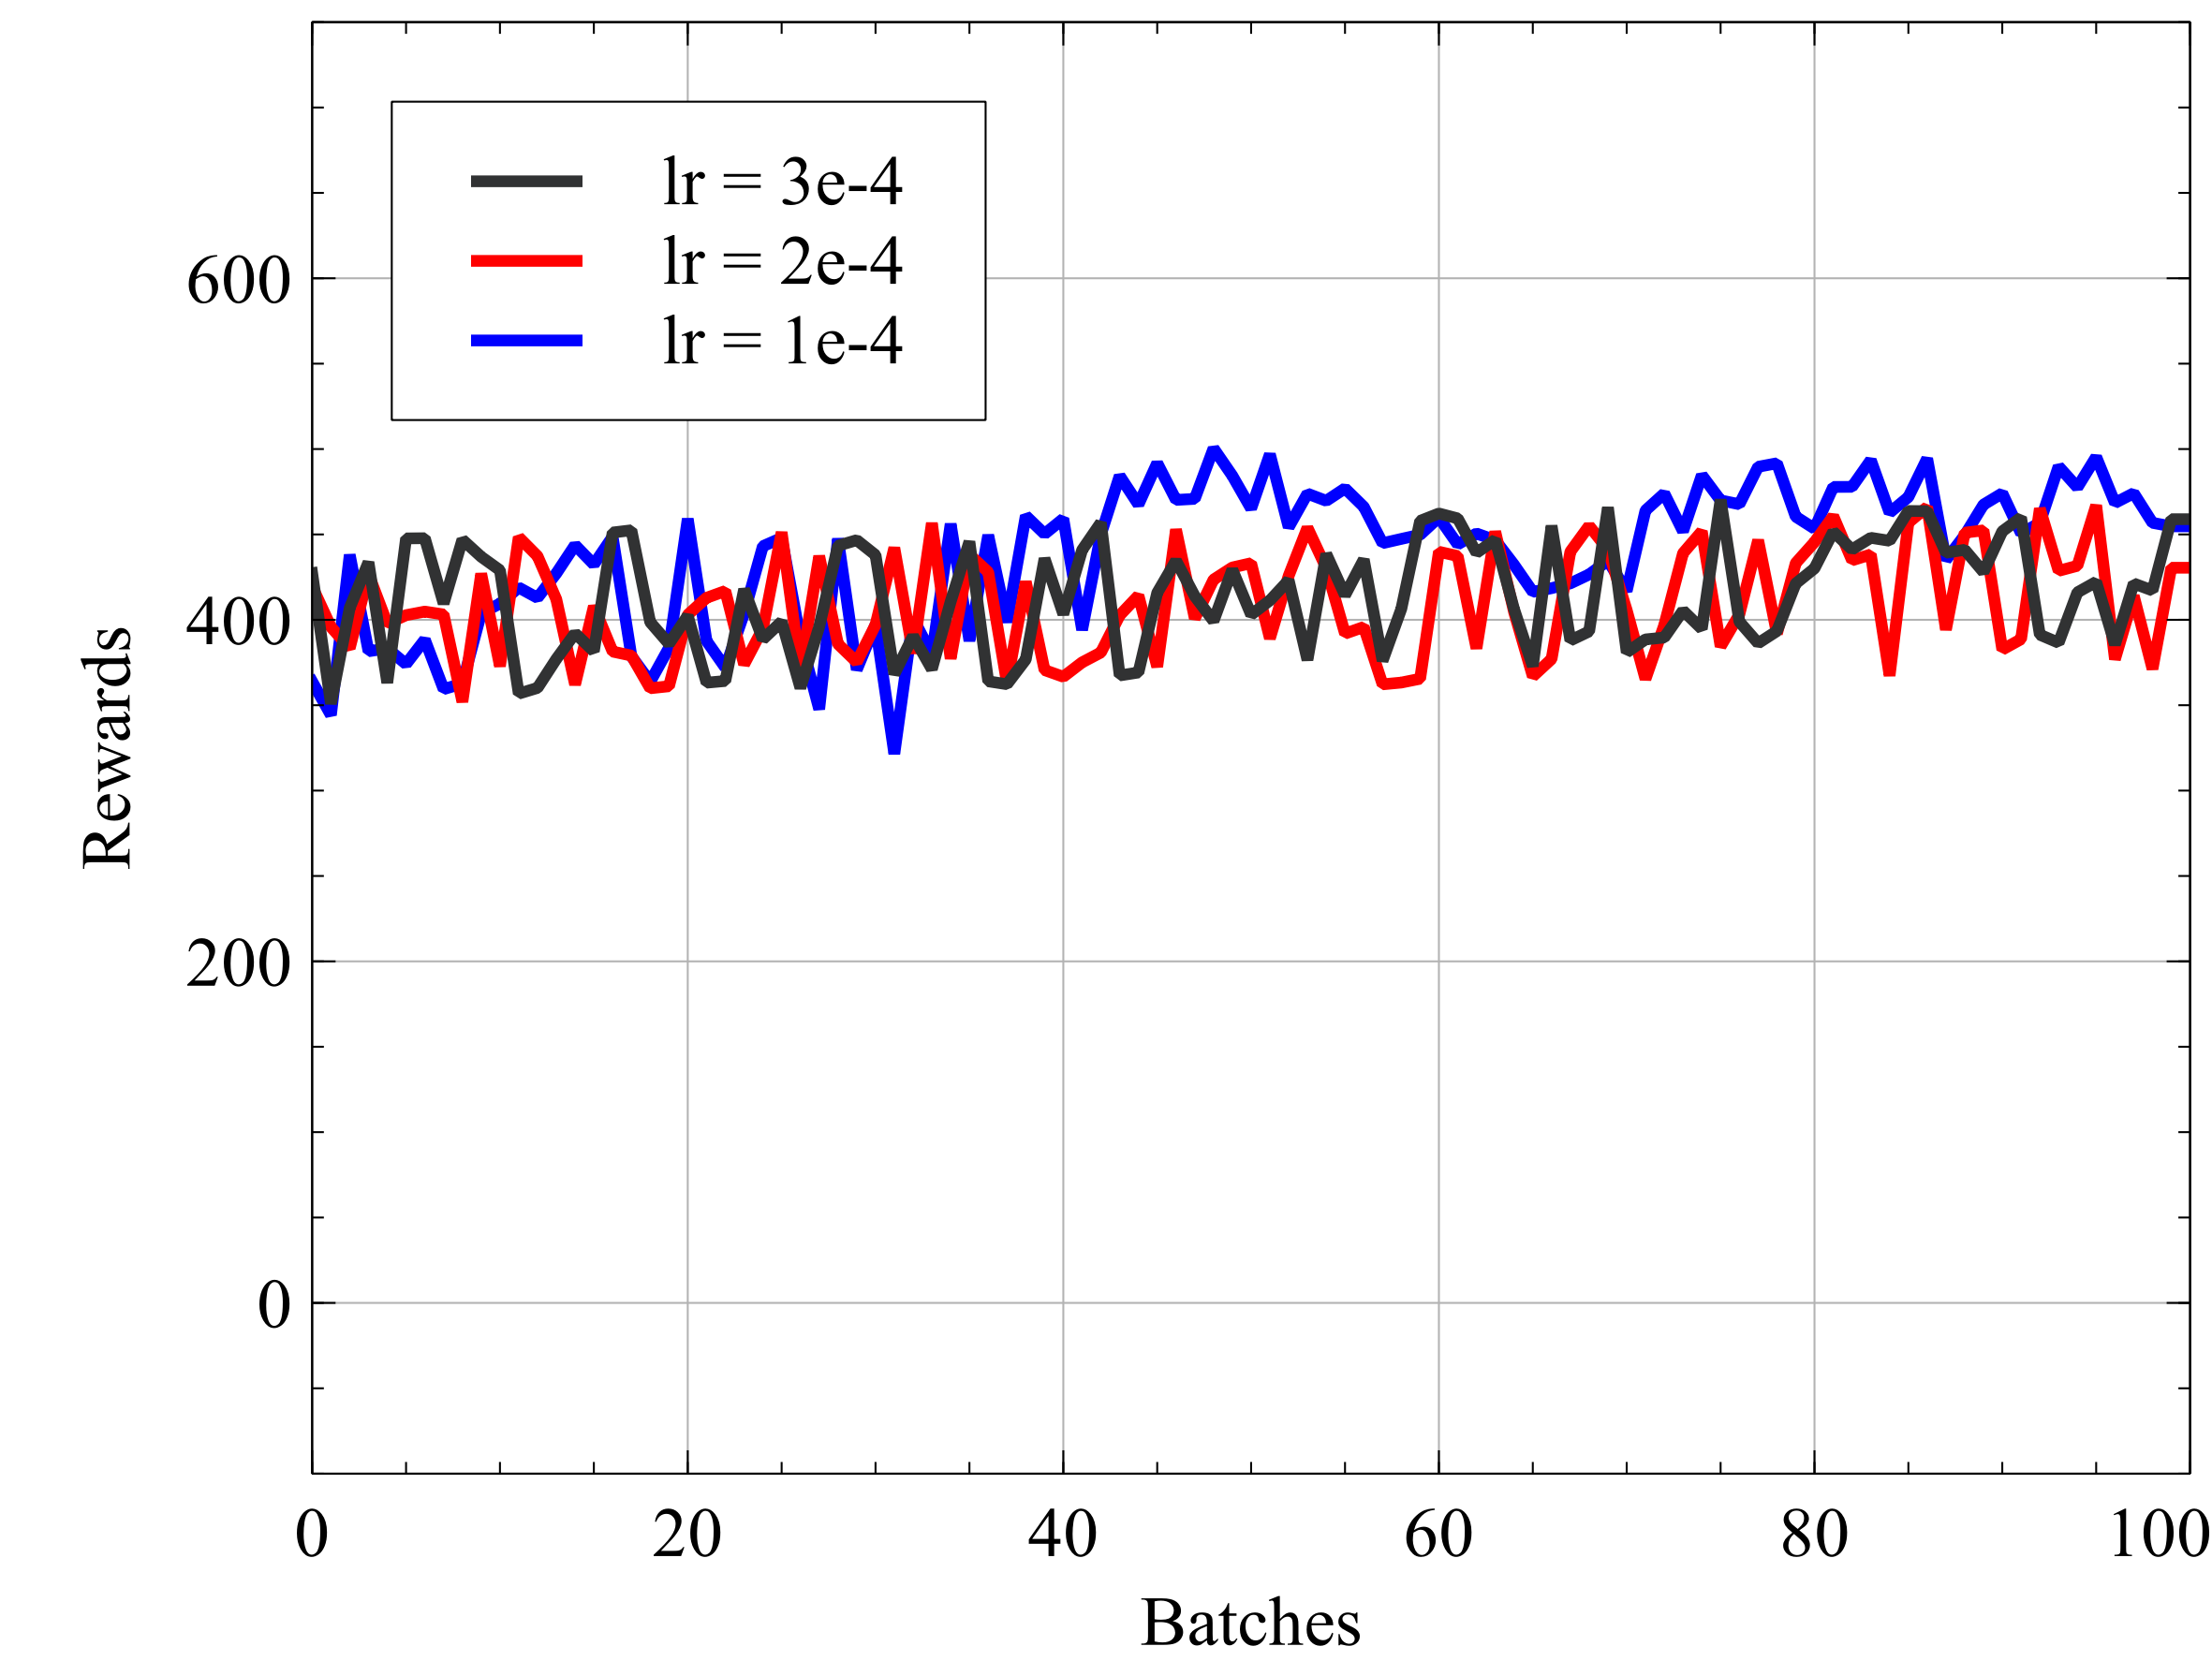
\includegraphics[width=0.42\textwidth]{./graphs/Results_08.png} \label{fig:g24}}
    \caption{The learning rate comparing graphs: Reward per batch on (a) Stage 1 and (b) Stage 2 in the precaching vehicle selection model; reward per batch on (c) Stage 1 and (d) Stage 2 in the precaching quantity decision model.}
\end{figure}
\subsection{Simulation results} \label{sec.s2}
In this subsection, we present the simulation results evaluating the performance of our proposed~SAC-PVS scheme.
We first compare model performance using reward per batch graphs for both stages of the precaching vehicle selection model and the precaching quantity decision model.
We then assess overall performance by examining two key metrics: total content download time and  wasted traffic, under varying conditions of requested content size, average vehicle speed, and vehicle density.
These results provide a comprehensive view of the efficacy and adaptability of the SAC-PVS scheme relative to alternative approaches.



\subsubsection{The learning curves}
Figure \ref{fig:g11} presents the reward per batch for Stage 1 of the precaching vehicle selection model, comparing the no ML scheme, the PPO scheme, and our proposed SAC scheme.
Overall, we observe that the SAC scheme's curve quickly rises and stabilizes at a higher reward, indicating more accurate vehicle selection over time, whereas the PPO scheme’s reward climbs more gradually, suggesting moderate adaptability.
The worst performance is seen in the no ML scheme, which remains near zero and never significantly improves; this outcome arises because the no ML scheme lacks any learning mechanism to adjust decisions in response to changing vehicular conditions, thus failing to capitalize on potential precaching opportunities.
Minor fluctuations observed in all schemes arise from inherent randomness in the simulation.
The PPO scheme steadily improves as it processes fresh batches of data; however, its on-policy nature limits sample efficiency and slows convergence, keeping its reward consistently below that of the SAC scheme.
By contrast, our proposed SAC scheme exploits off-policy learning and entropy regularization, enabling effective reuse of past experiences and maintaining an optimal balance between exploration and exploitation, ultimately achieving the highest reward in dynamic CIoV scenarios.

Figure \ref{fig:g12} presents the reward per batch for Stage 2 in the precaching vehicle selection model, comparing the no ML scheme, the PPO scheme, and our proposed SAC scheme.
Overall, the SAC scheme demonstrates a rapid increase in reward and consistently maintains higher values, reflecting its ability to fine-tune the vehicle selection process more effectively.
In contrast, the no ML scheme exhibits persistently low rewards, indicating that its static optimization cannot adapt to dynamic vehicular environments, resulting in less effective selection decisions.
The PPO scheme, though improving over time, remains in the middle range because its on-policy nature limits data reuse and slows convergence, preventing it from reaching the SAC scheme’s performance.
By leveraging off-policy learning and entropy regularization, the SAC approach efficiently reuses past experiences while maintaining robust exploration, thus consistently outperforming the other methods in this second stage of vehicle selection.

Figure \ref{fig:g13} depicts the reward per batch for Stage 1 of the precaching quantity decision model, comparing the no ML scheme, the PPO scheme, and our SAC scheme.
The SAC scheme rapidly escalates to a higher reward plateau, demonstrating its effectiveness in determining appropriate precaching amounts.
The no ML scheme remains near the bottom, indicating that a purely mathematical optimization cannot adapt to shifting vehicle and content demands.
The PPO scheme, while it eventually surpasses the no ML scheme, lags behind the SAC scheme due to its reliance on on-policy updates, which limits the reuse of past data.
By leveraging off-policy learning and maintaining a balance between exploration and exploitation, the SAC scheme consistently achieves superior performance in deciding the appropriate amount of content to precache for each vehicle.

Figure \ref{fig:g14} presents the reward per batch for Stage 2 of the precaching quantity decision model, comparing the no ML scheme, the PPO scheme, and our SAC scheme are compared.
Stage 2 of the precaching quantity decision model has already been heavily trained by the previous step, so the graph shows some convergence.
The no ML scheme remains consistently low, reflecting the inability of static mathematical optimization struggles to keep pace with evolving conditions.
The PPO scheme demonstrates moderate improvement but still lags behind the SAC scheme, which achieves the highest rewards by effectively leveraging off-policy learning and strategic exploration.
By adaptively fine-tuning content allocation, the SAC scheme efficiently balances caching overhead and successful delivery, achieving superior performance in this second stage of the precaching quantity decision process.
\begin{figure}[H]
    \centering
    \subfigure[]{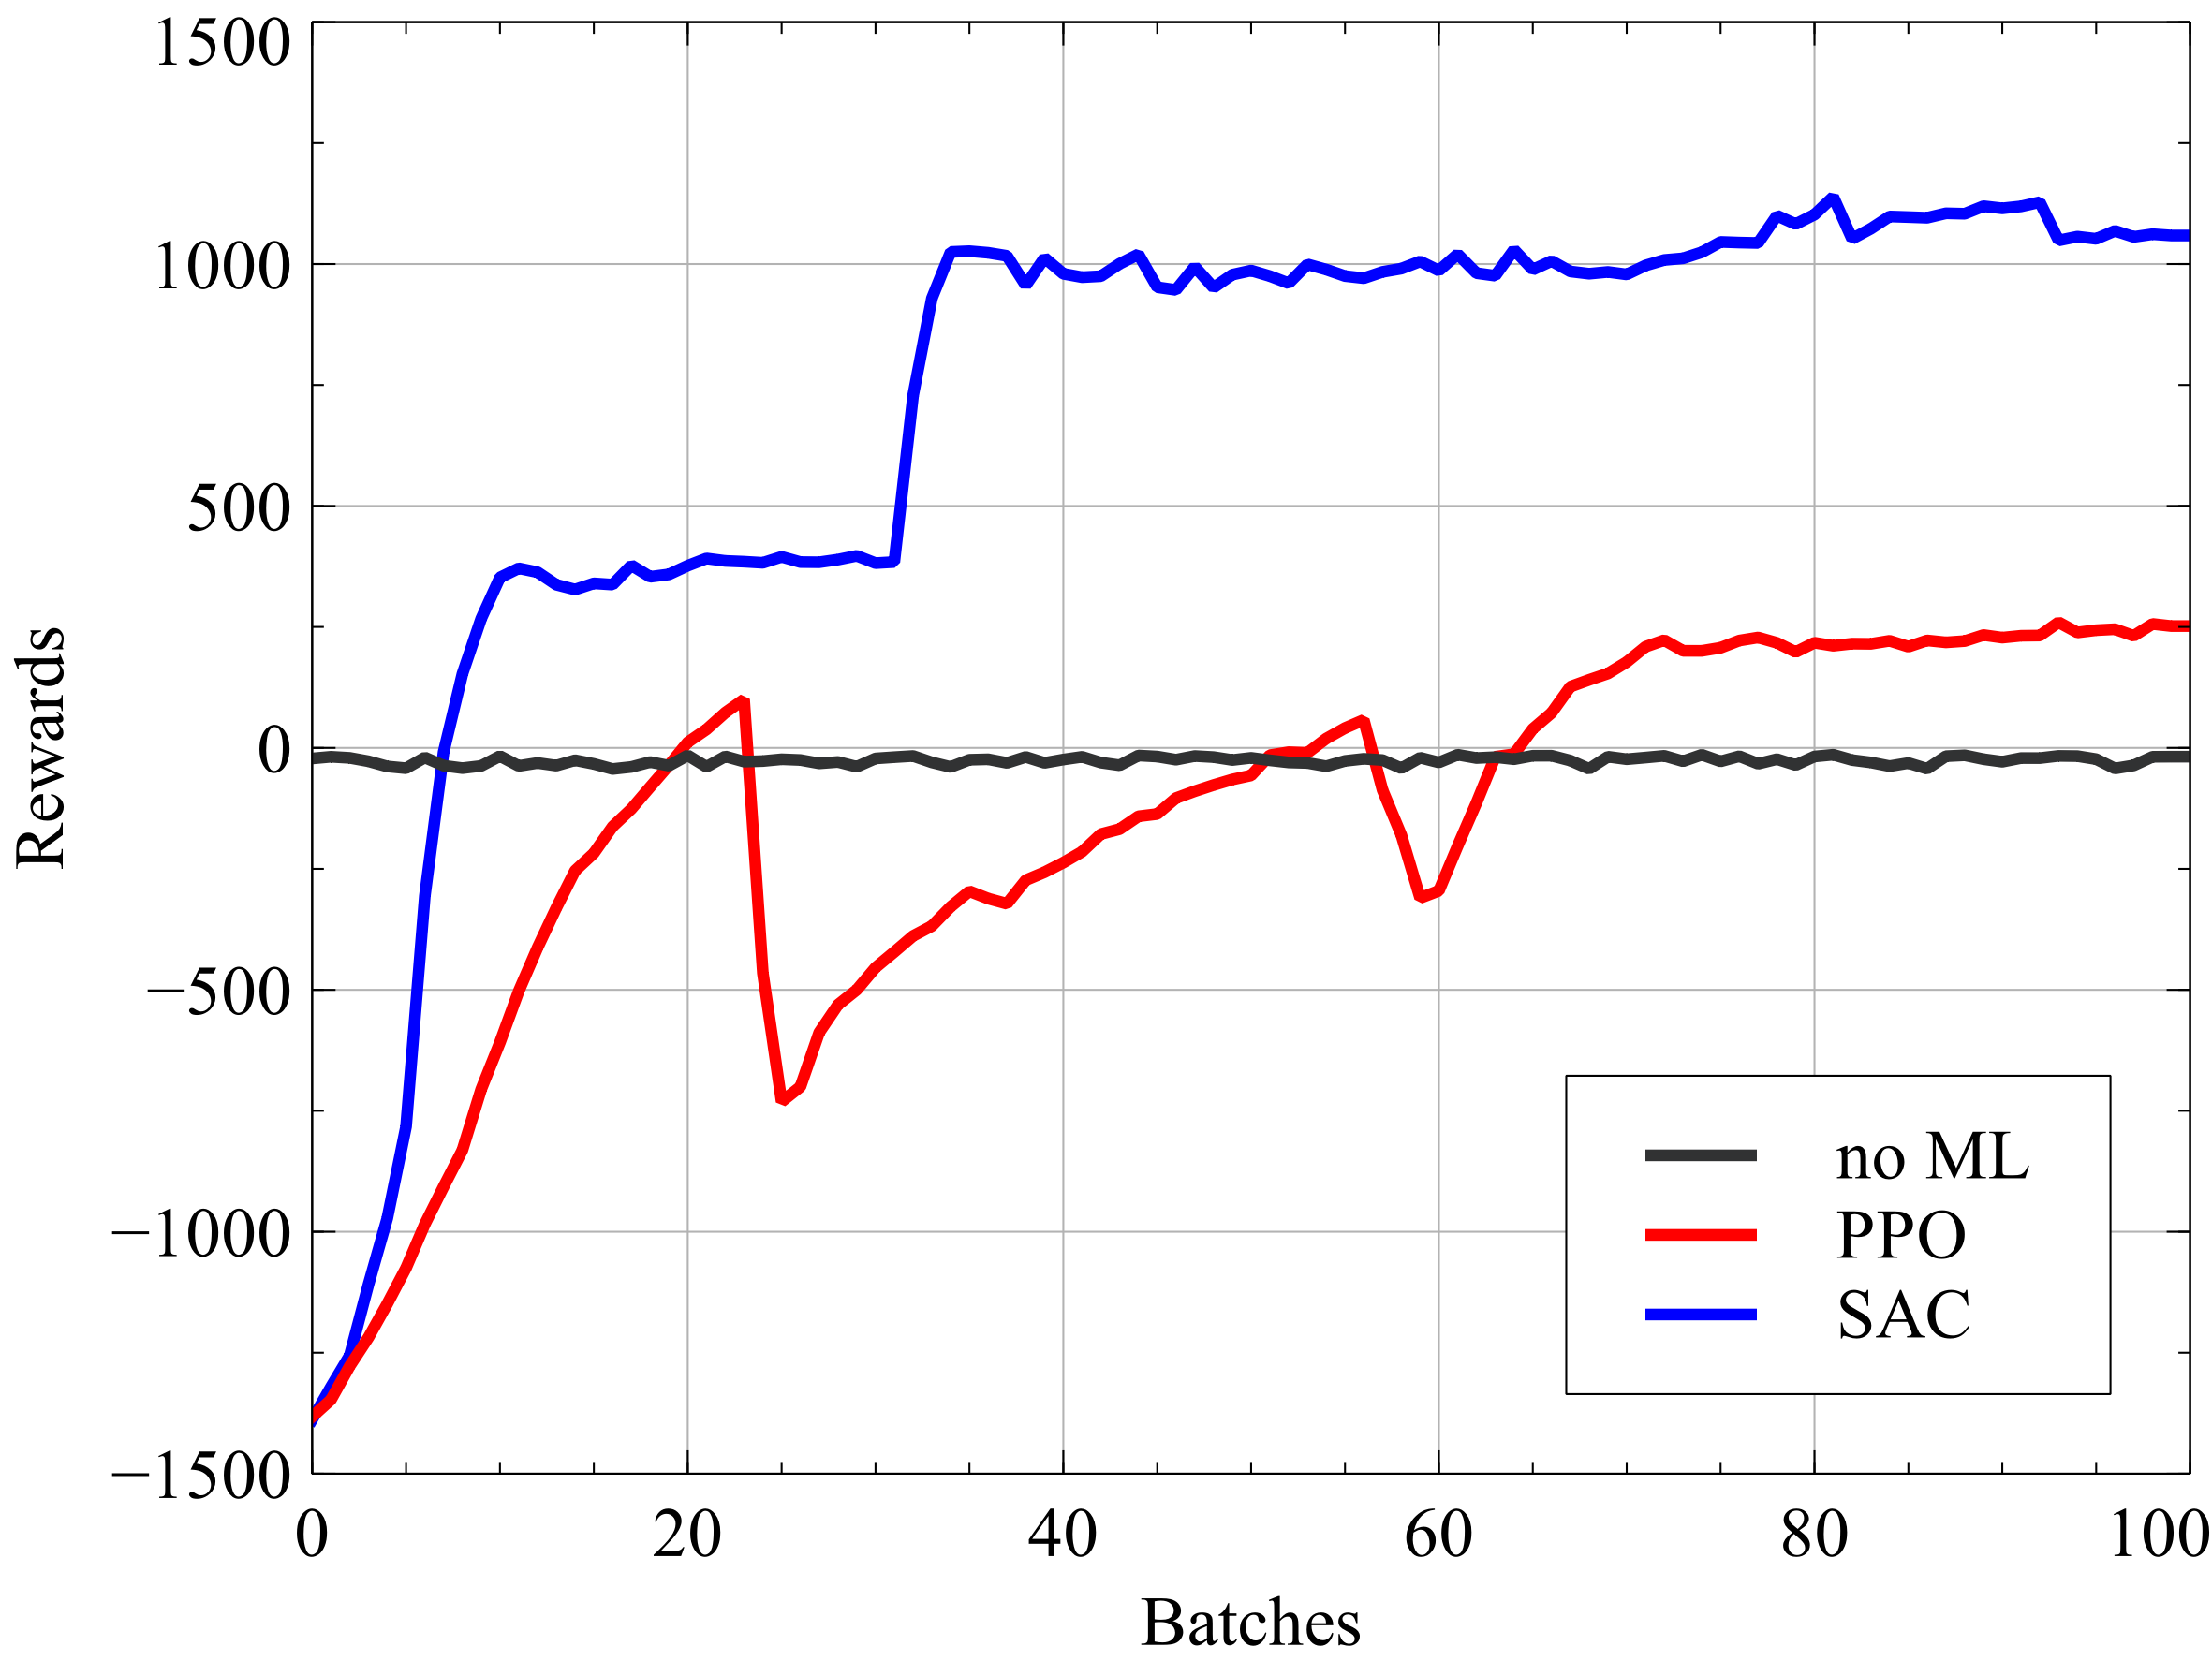
\includegraphics[width=0.45\textwidth]{./graphs/Results_01.png} \label{fig:g11}}
    \subfigure[]{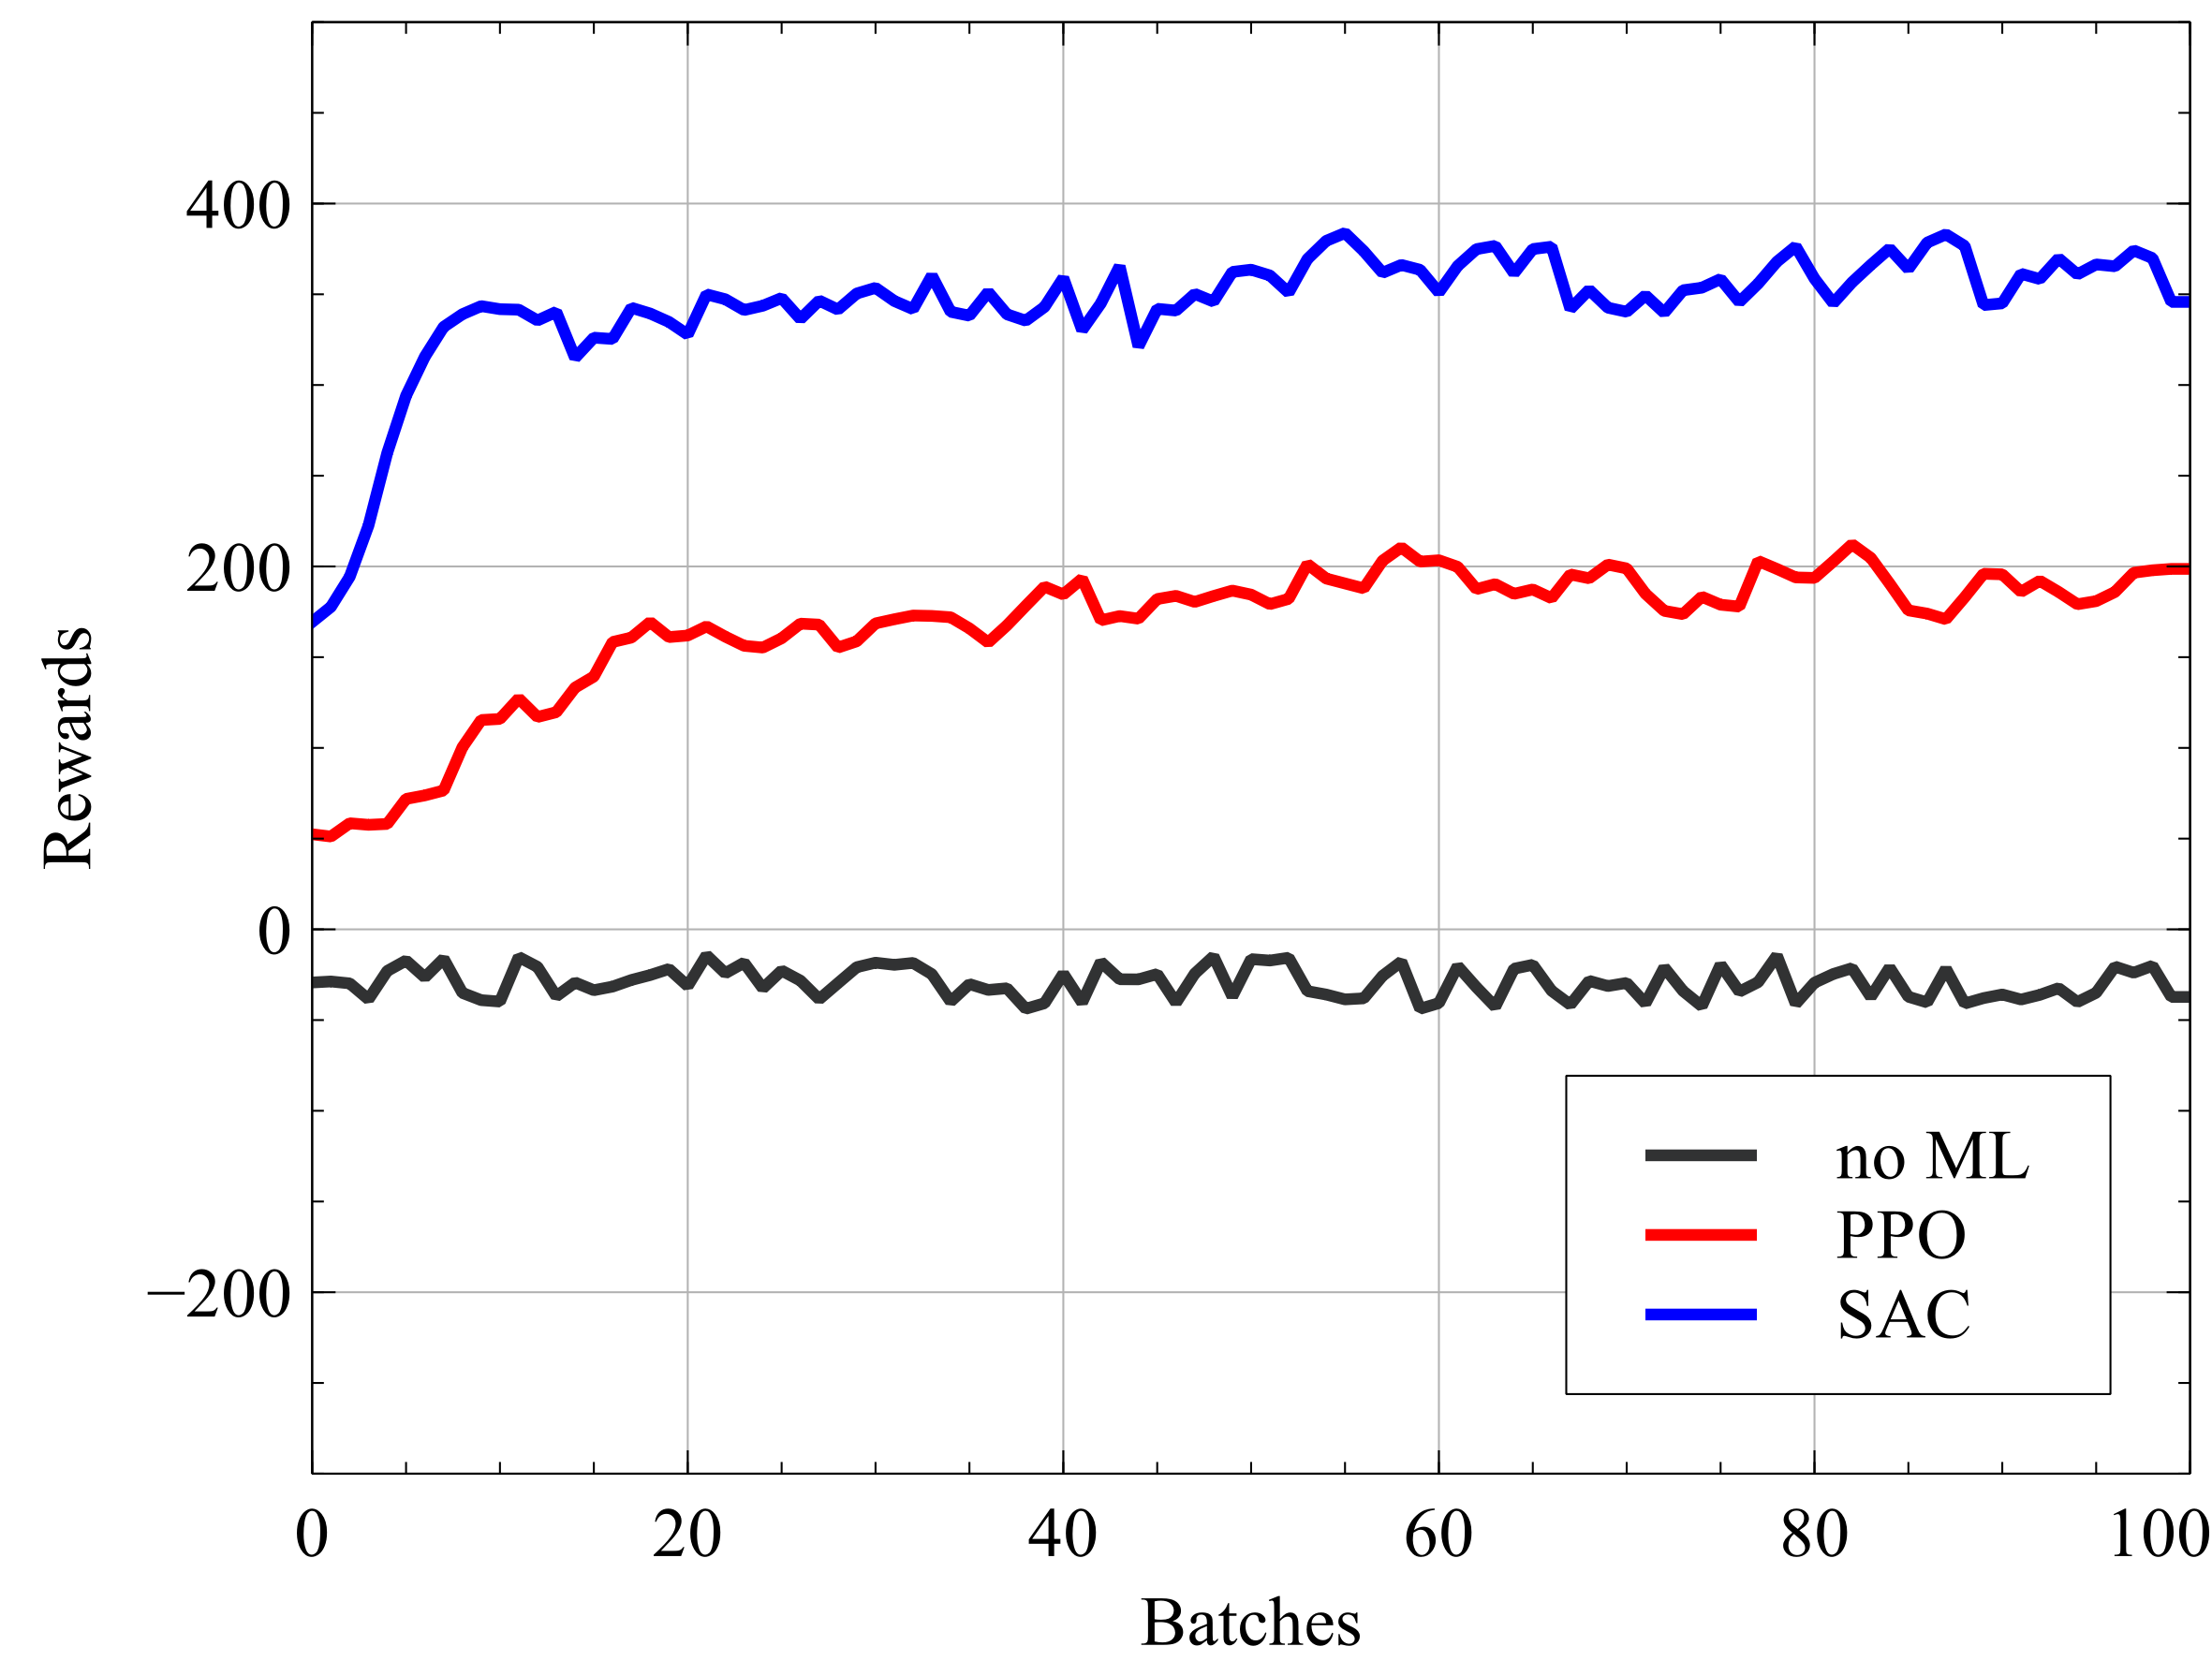
\includegraphics[width=0.45\textwidth]{./graphs/Results_02.png} \label{fig:g12}}\\
    \subfigure[]{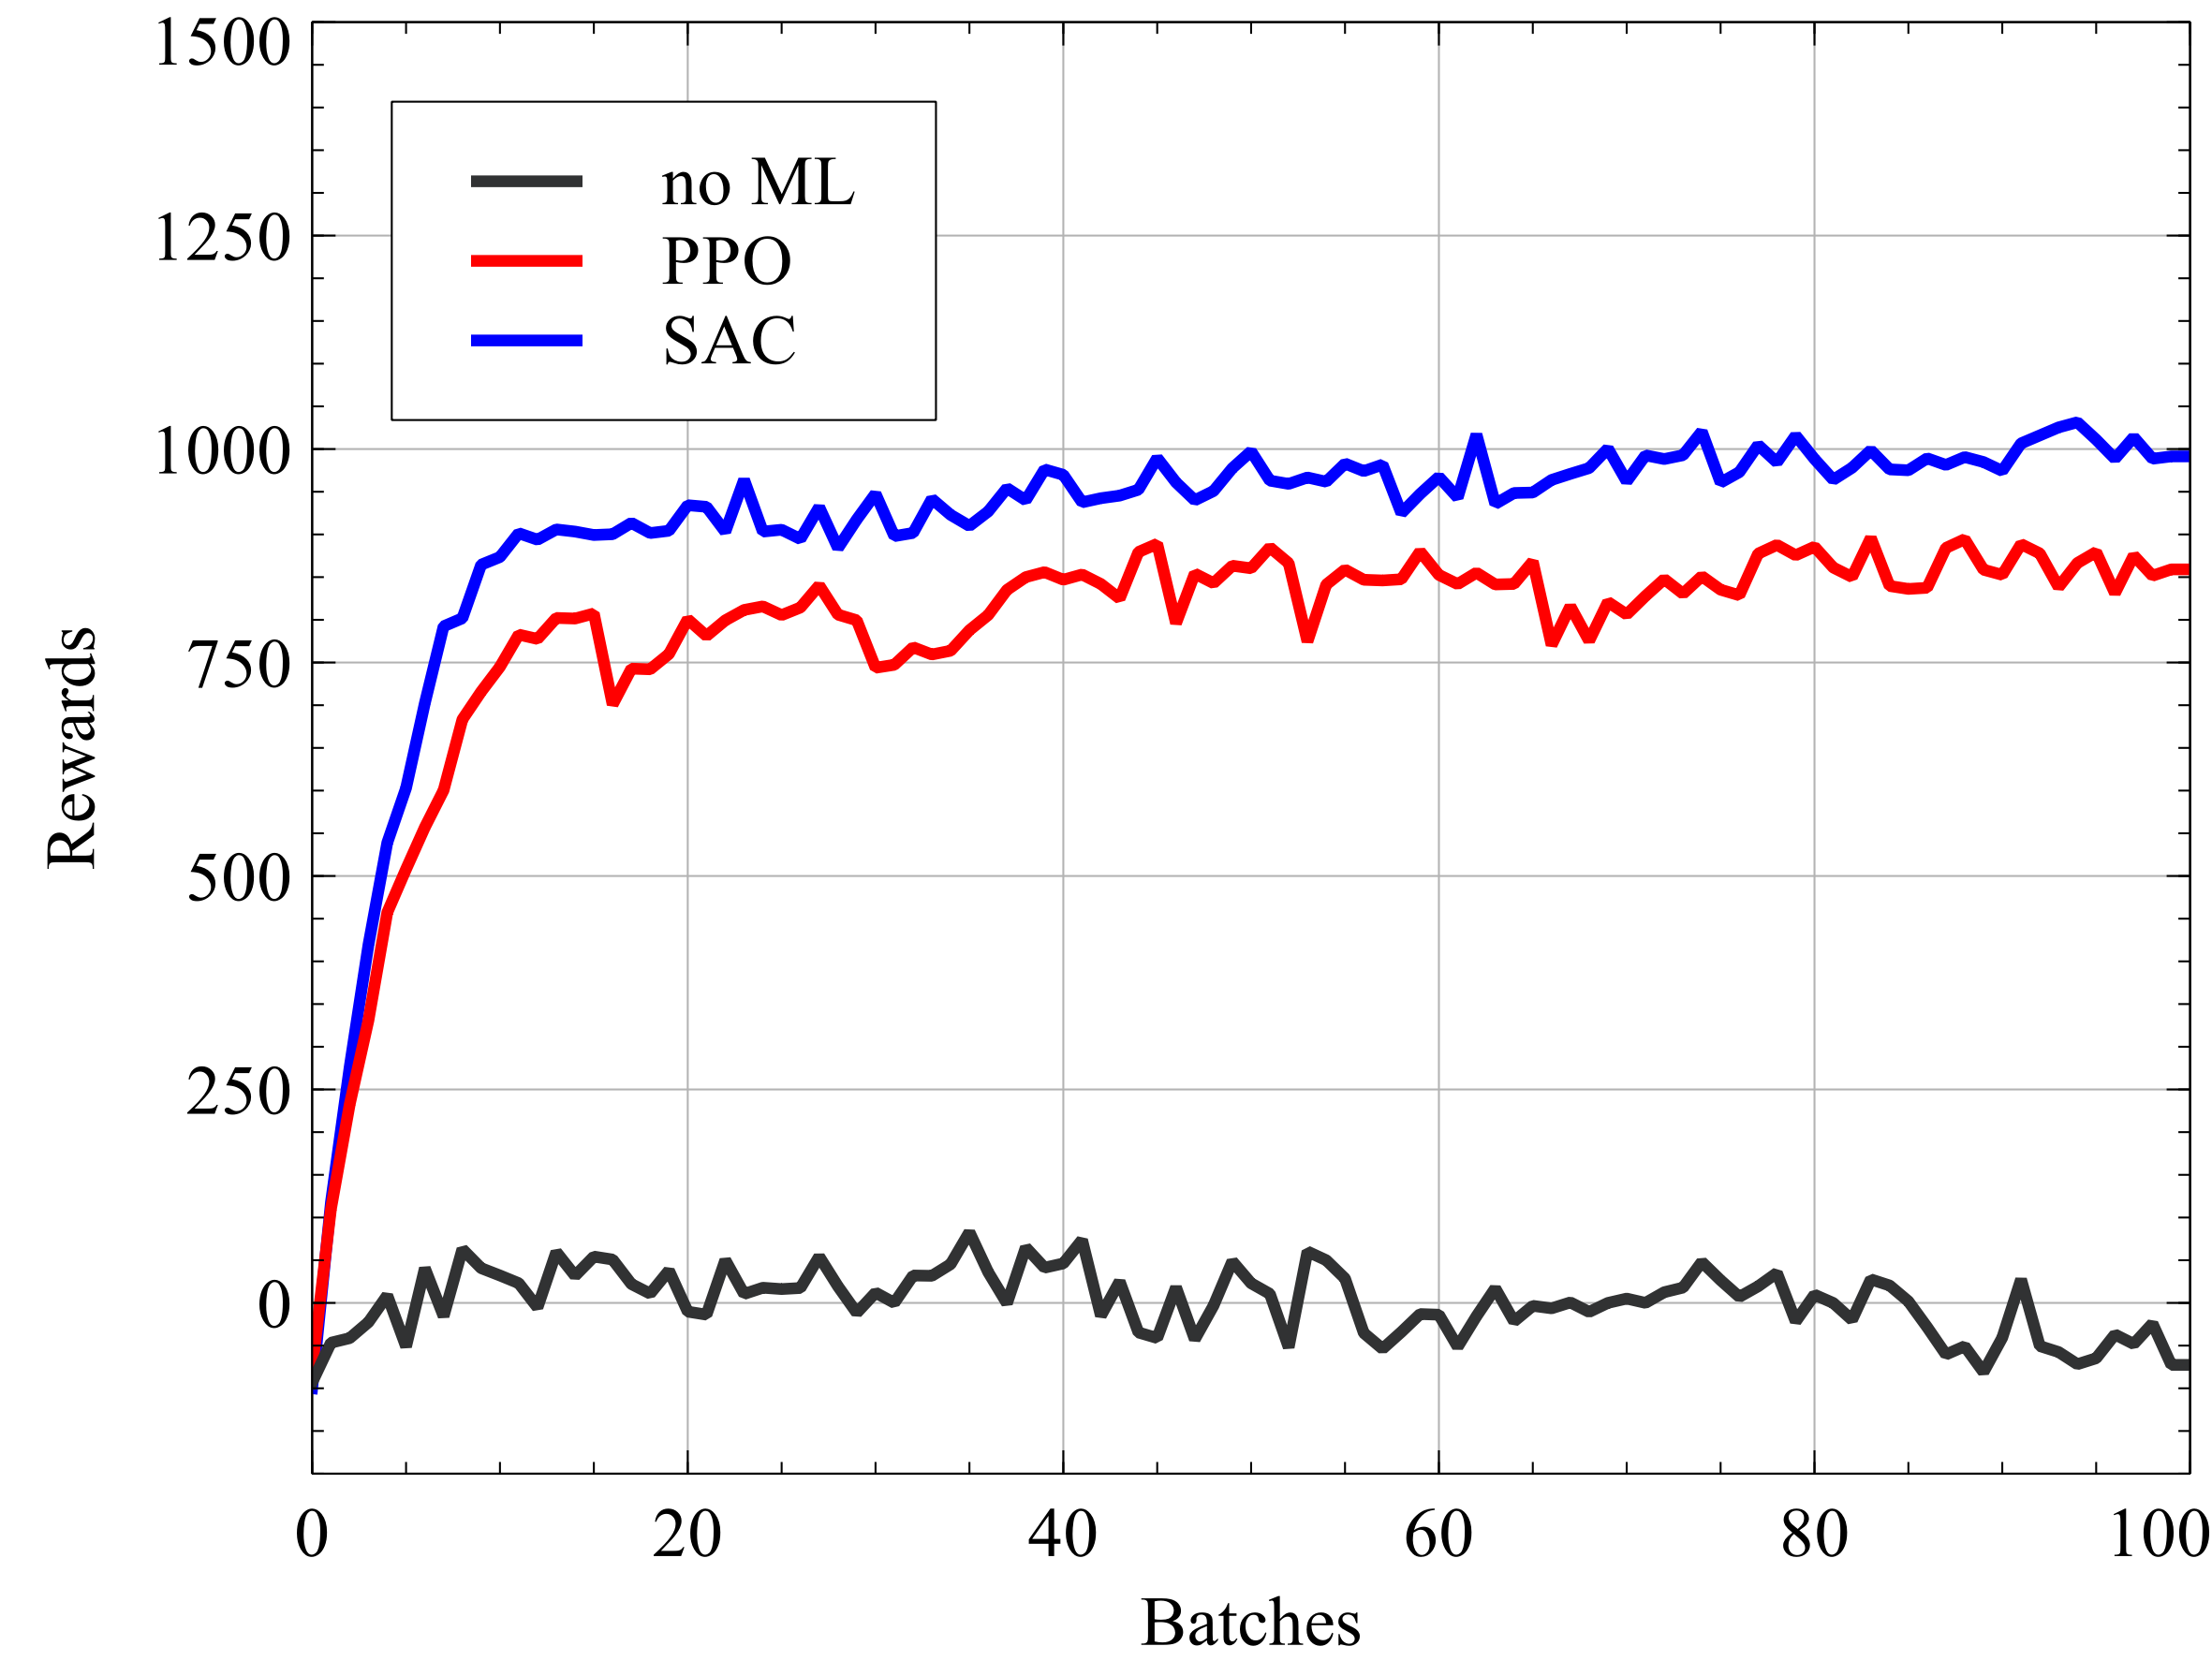
\includegraphics[width=0.45\textwidth]{./graphs/Results_05.png} \label{fig:g13}}
    \subfigure[]{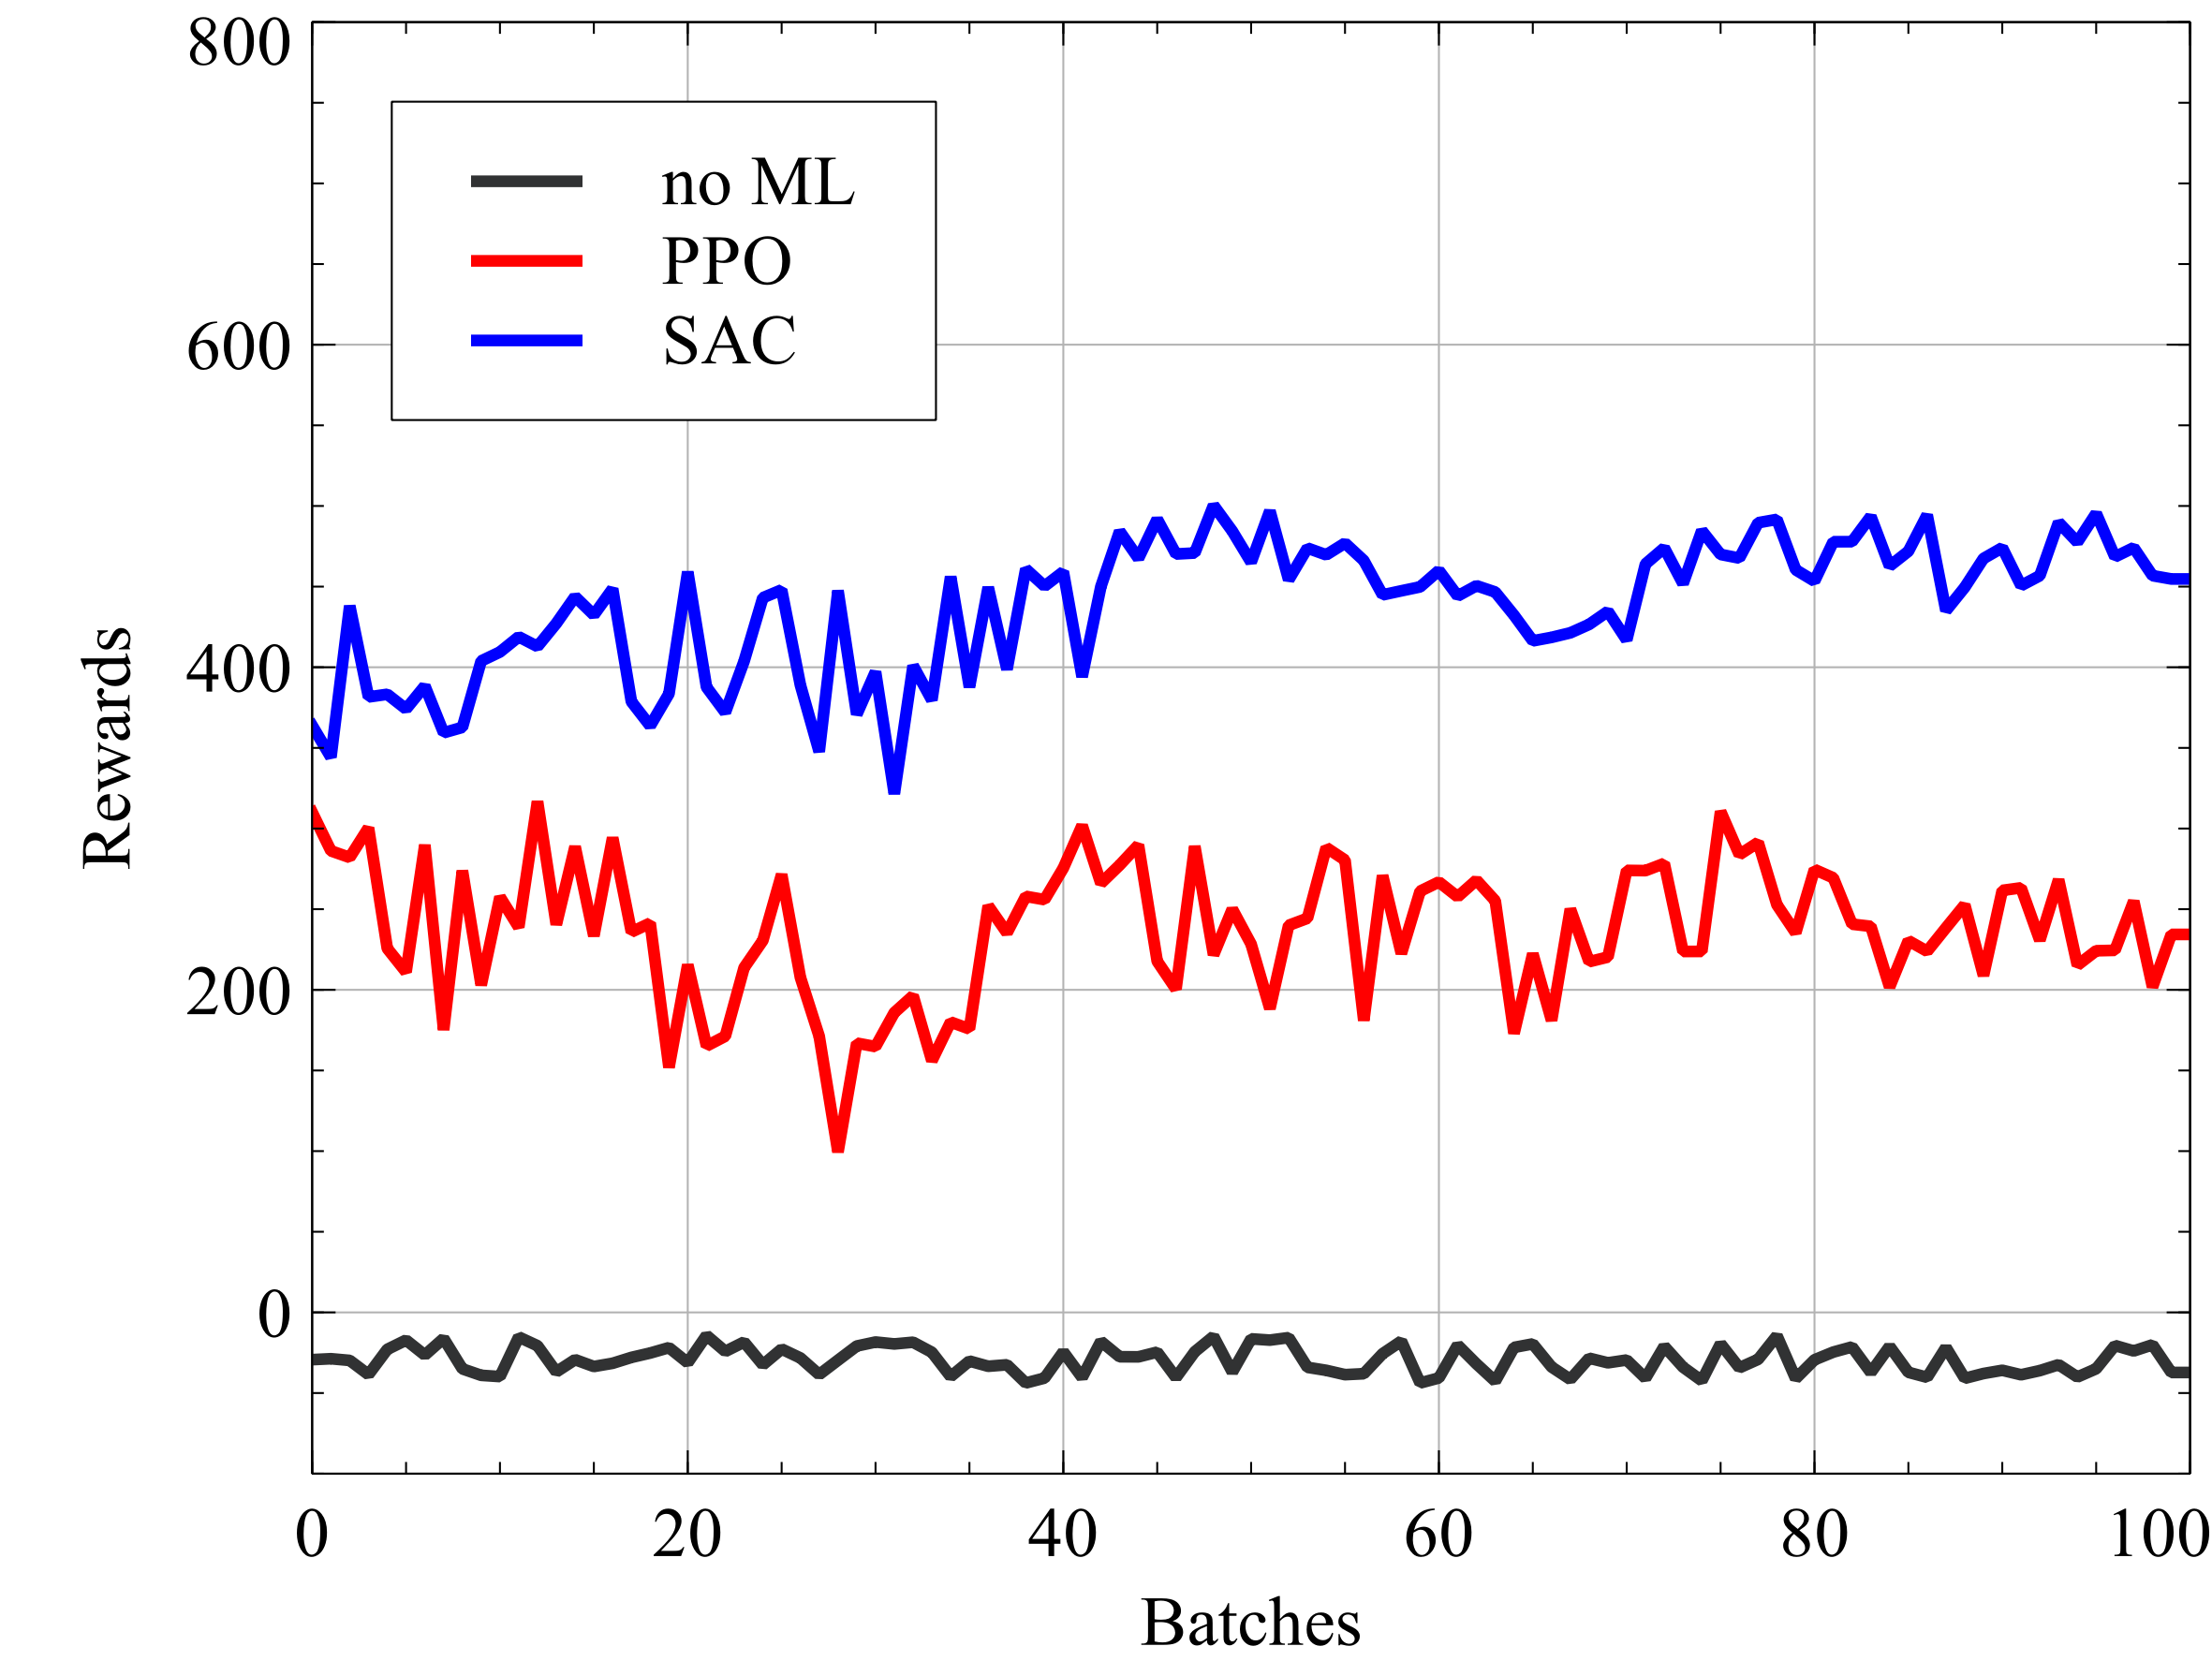
\includegraphics[width=0.45\textwidth]{./graphs/Results_06.png} \label{fig:g14}}
    \caption{The model comparing graphs: reward per batch on (a) Stage 1 and (b) Stage 2 in the precaching vehicle selection model; reward per batch on (c) Stage 1 and (d) Stage 2 in the precaching quantity decision model.}
\end{figure}
\newpage


\subsubsection{The total content download time graphs}
Figure \ref{fig:g31} shows the total content download time as the requested content size increases, with the no ML scheme, the PPO scheme, and the SAC scheme.
Although the difference among these approaches may appear small on the large y-axis scale, they actually diverge by tens of seconds in some intervals.
The overall upward trend is represented, as larger content volumes naturally take longer to transmit.
The no ML scheme exhibits the highest times, reflecting its static strategy’s inability to adapt to growing content demands.
The PPO scheme performs moderately but lags behind. In contrast, the~SAC scheme consistently achieves the lowest download times.
This robustness is attributed to our snapshot-based design; regardless of sudden changes in content popularity or request size, the agent optimizes the immediate delivery path without relying on long-term popularity prediction, making it resilient to demand fluctuations.

Figure \ref{fig:g32} illustrates the total content download time in relation to the average speed of vehicles, comparing the no ML scheme, the PPO scheme, and the SAC scheme.
Overall, the curves descend at moderate speeds and then stabilize, indicating that there is a spot where vehicles spend enough time within RSU range to complete downloads efficiently without incurring excessive handovers.
The no~ML scheme consistently shows higher download times because it cannot adapt its caching decisions to changes in vehicle speed.
The PPO scheme demonstrates improved adaptation but struggles under high mobility.
In contrast, the SAC scheme maintains the lowest download times even at high speeds.
In these extreme high-mobility scenarios, where network topology changes rapidly, SAC's continuous action space allows for fine-grained adjustments in vehicle selection, maintaining stable connectivity where discrete or static methods fail.

Figure \ref{fig:g33} shows the total content download time as vehicle density increases, comparing the no ML scheme, the PPO scheme, and the SAC scheme.
All curves trend downward, indicating that a higher density of vehicles can improve content delivery by increasing the opportunities for V2V communication.
The no ML scheme remains at the highest download times due to its static approach, which does not adapt to the additional vehicles available for content sharing.
While PPO improves over the baseline, the SAC scheme outperforms it, particularly in sparse vehicle density scenarios.
In these extreme conditions, where caching candidates are limited, optimal vehicle selection becomes critical.
SAC effectively identifies the few viable vehicles to bridge the connectivity gap, preventing delivery failures.
\newpage
\begin{figure}[H]
    \centering
    \subfigure[]{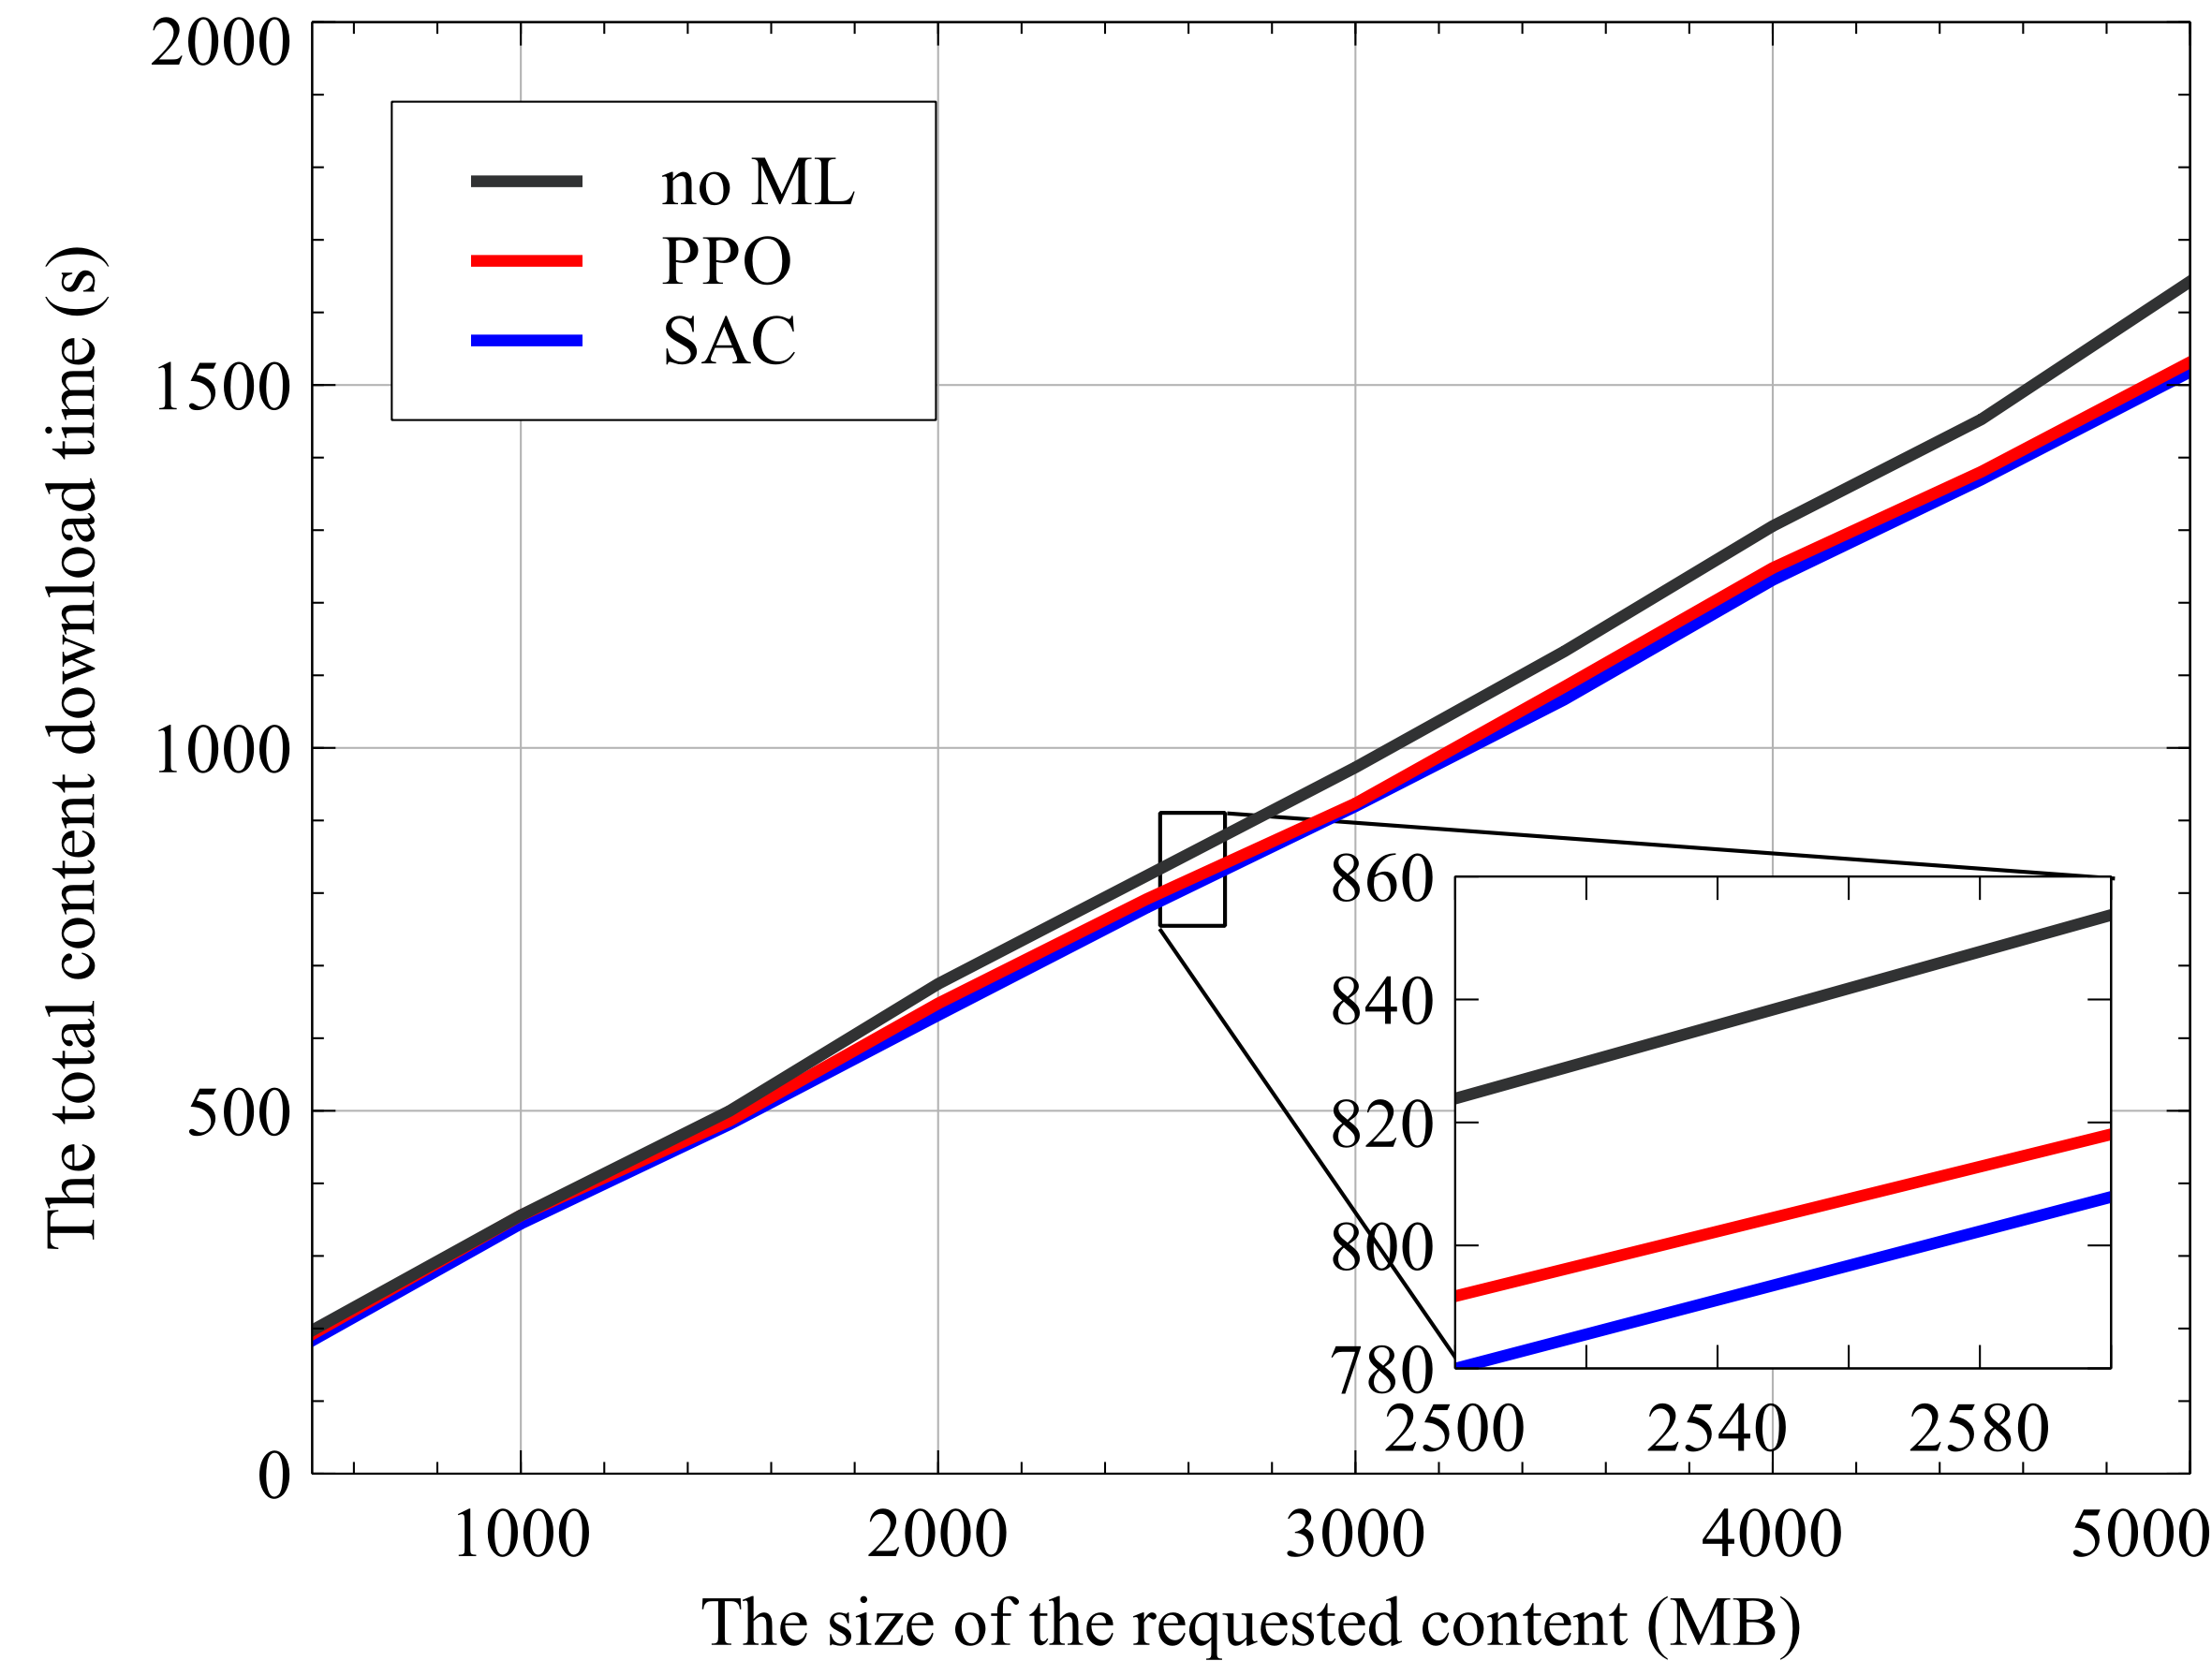
\includegraphics[width=0.45\textwidth]{./graphs/Results_09.png}
    \label{fig:g31}}
    \subfigure[]{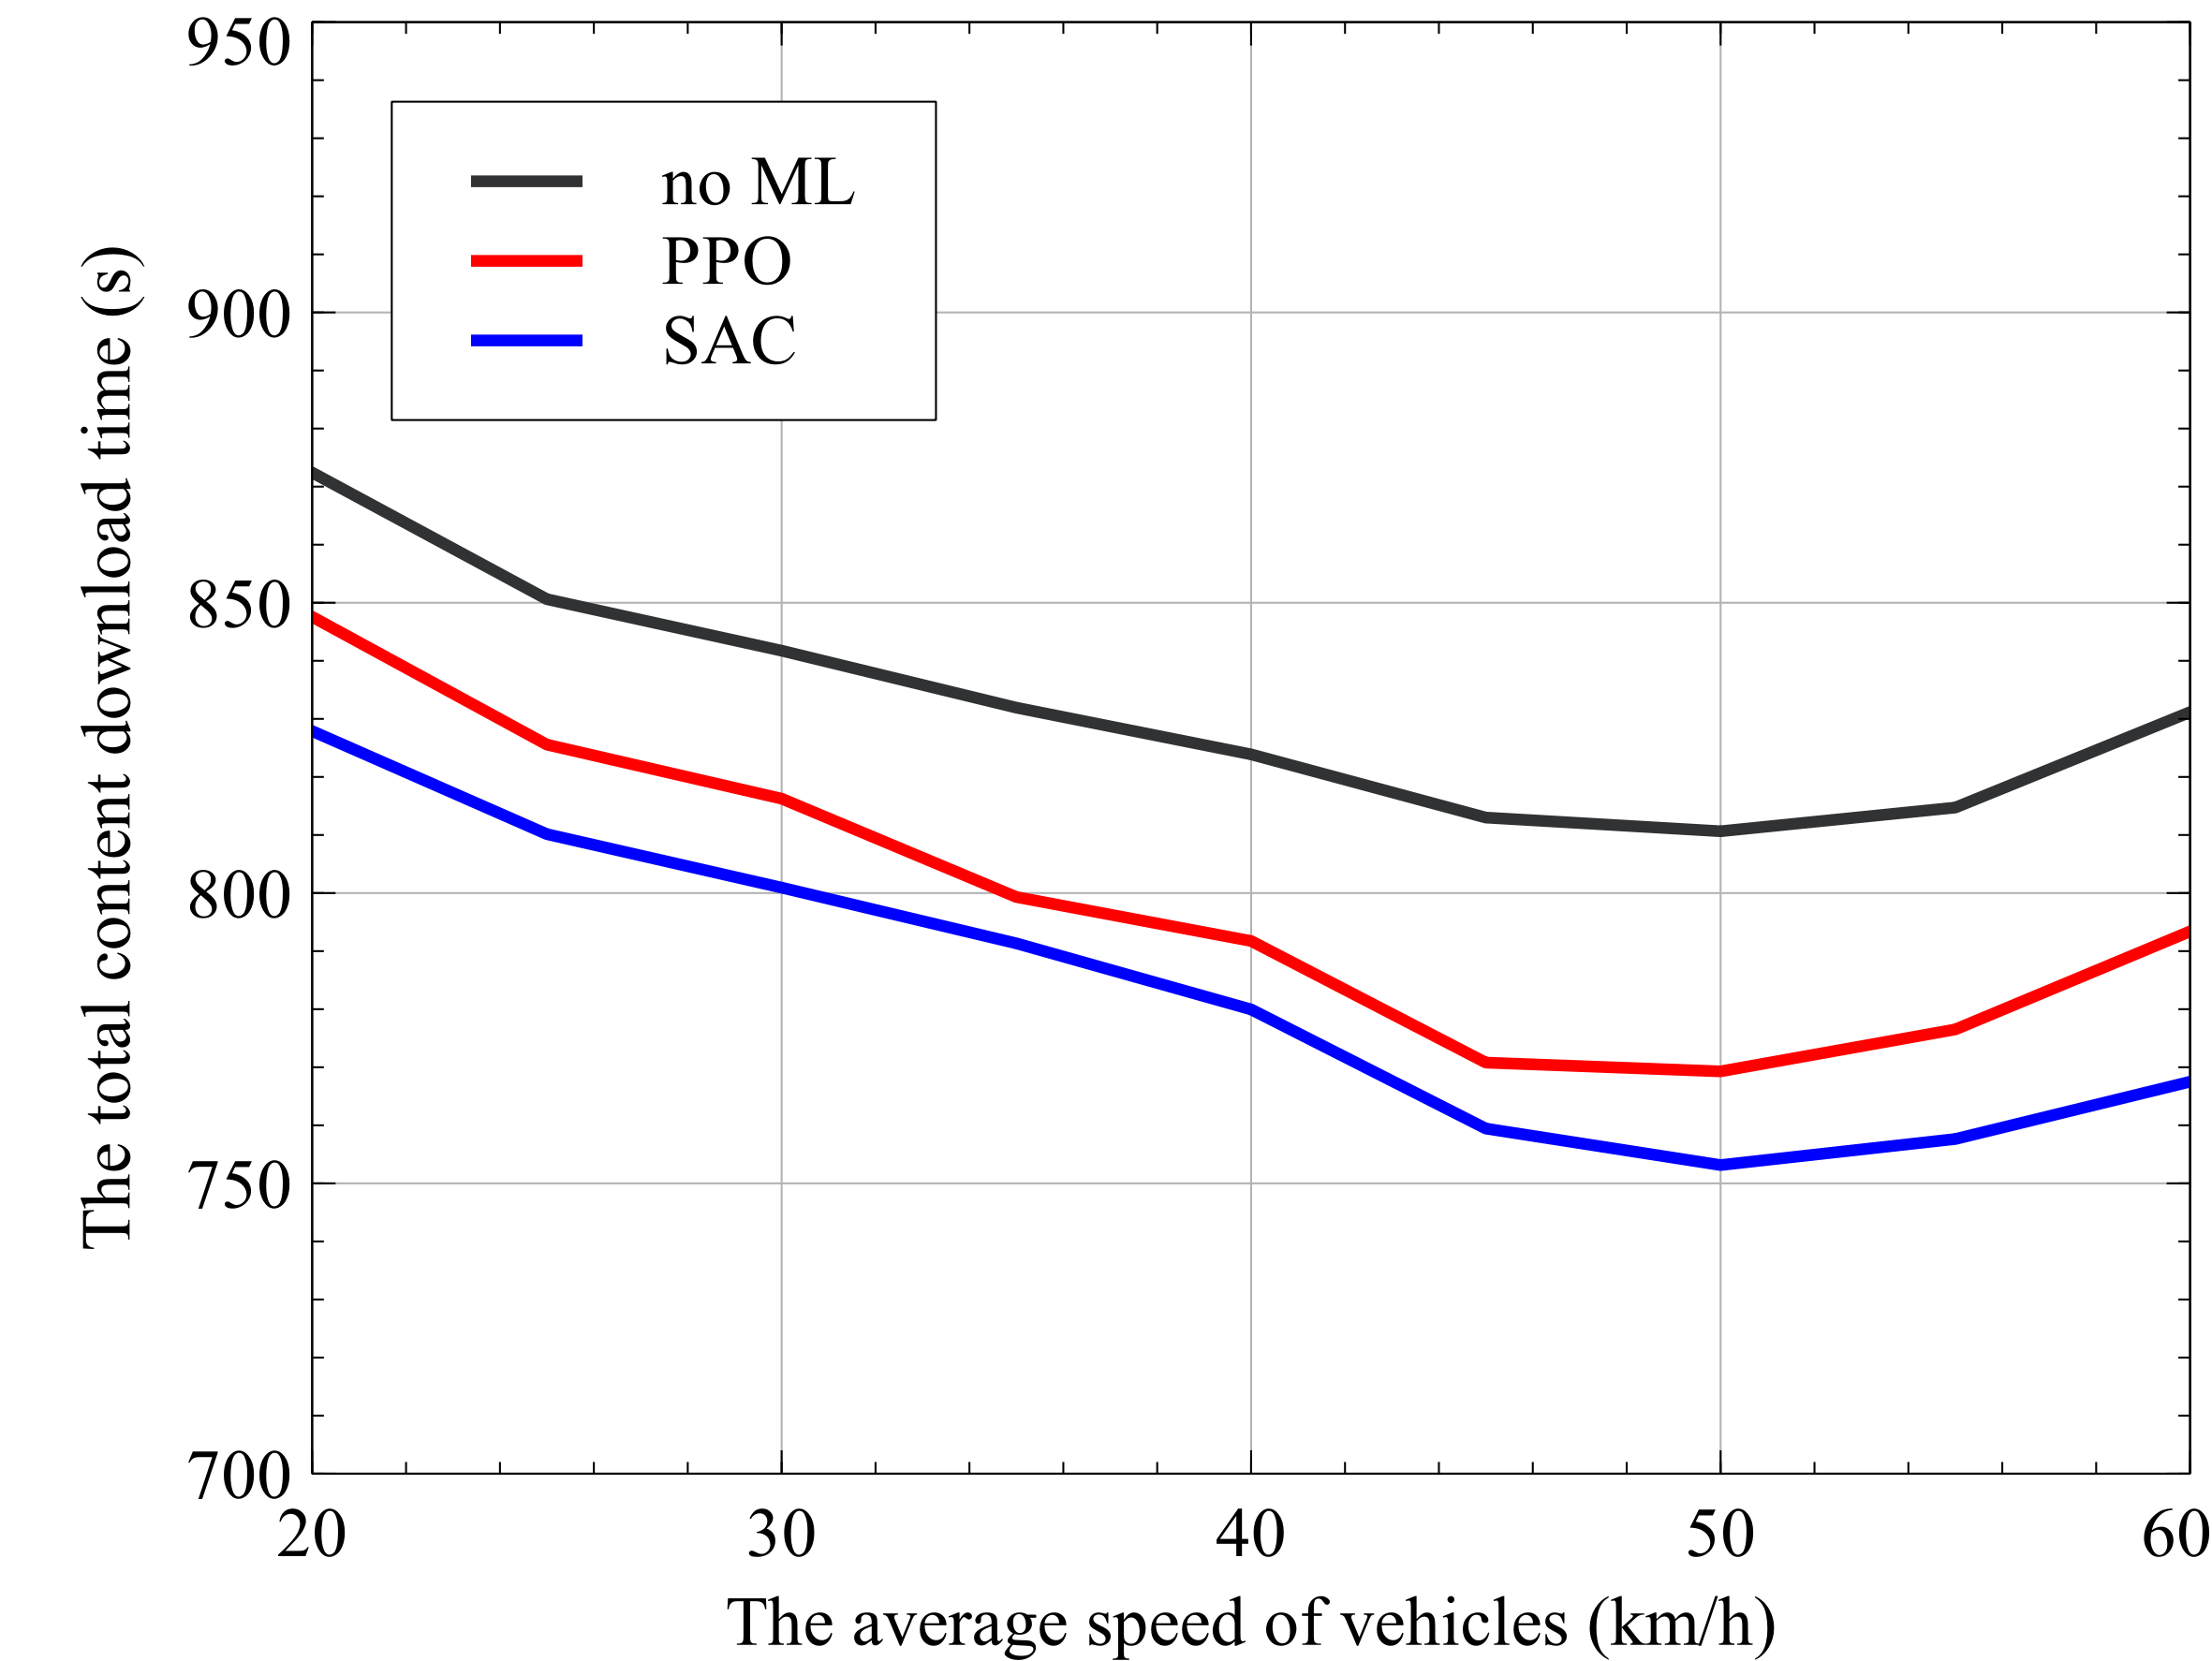
\includegraphics[width=0.45\textwidth]{./graphs/Results_11.png}
    \label{fig:g32}}\\
    \subfigure[]{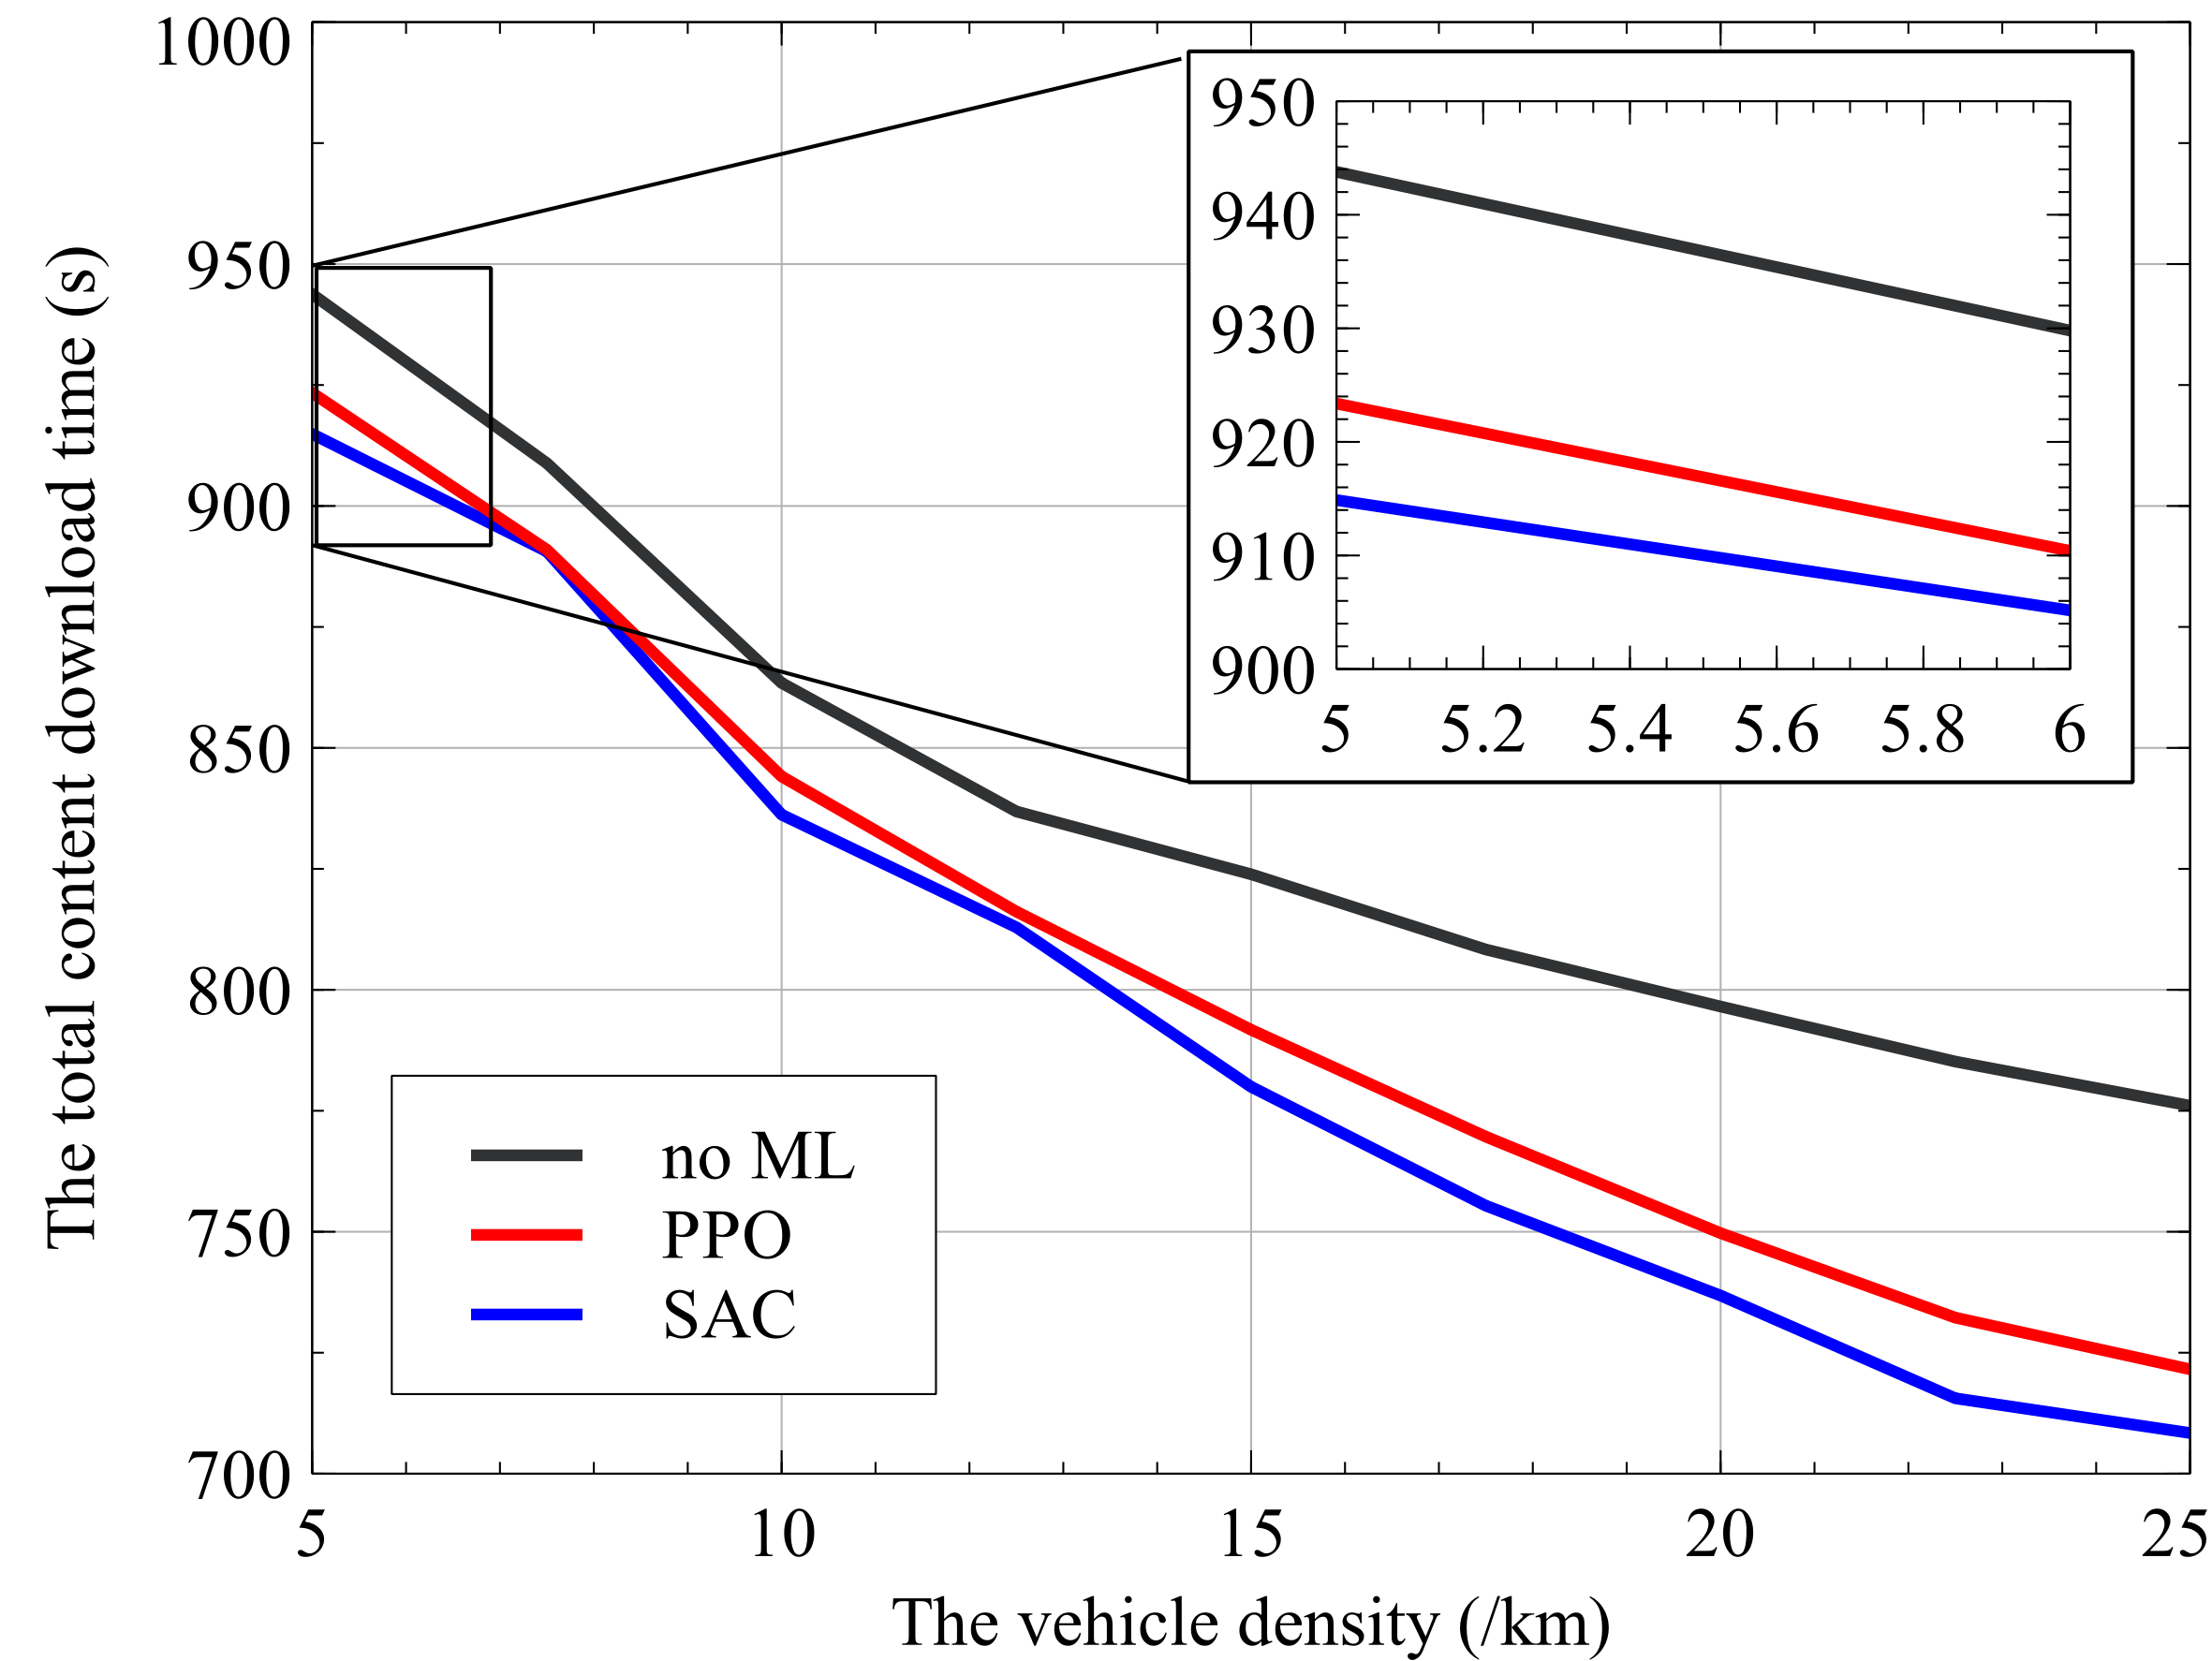
\includegraphics[width=0.45\textwidth]{./graphs/Results_13.png}
    \label{fig:g33}}
    \caption{The total content download time according to (a) the size of the requested content, (b) the average speed of vehicles, and (c) the vehicle density.}
\end{figure}


\subsubsection{The wasted traffic graphs}
Figure \ref{fig:g41} illustrates wasted traffic as the requested content size increases.
All curves trend upward, reflecting the higher risk of over-caching as content sizes grow.
The no ML scheme shows the steepest rise due to its inability to adjust caching amounts.
The PPO scheme performs better but still results in higher waste.
In contrast, the SAC scheme maintains the lowest wasted traffic.
This is achieved by the specific design of our precaching quantity decision stage, which predicts the exact amount of chunks needed.
This precise control prevents the all-or-nothing caching often seen in discrete action spaces, significantly reducing waste even when handling large content files.

Figure \ref{fig:g42} shows wasted traffic as a function of the average speed of vehicles.
As vehicle speed increases, the contact duration for reliable transmission decreases, increasing the risk of failed deliveries turning into wasted traffic.
The no ML scheme exhibits the highest waste, while PPO reduces it moderately.
In contrast, the SAC scheme effectively minimizes waste even at high speeds.
By incorporating mobility patterns and contact durations into its continuous state space, SAC avoids caching content on vehicles likely to move out of range too quickly, a critical capability for robustness in high-mobility scenarios.

Figure \ref{fig:g43} shows how wasted traffic changes with increasing vehicle density.
All lines ascend as more vehicles become available, raising the likelihood of redundant caching.
The no ML and~PPO schemes struggle to filter out unnecessary candidates in crowded environments.
Conversely, the~SAC scheme maintains the lowest overall waste.
Its vehicle selection stage acts as an effective filter, choosing only the optimal subset of vehicles for precaching rather than broadcasting to all available neighbors.
This selective approach proves its efficiency particularly in dense network environments where redundancy is a major concern.
\begin{figure}[H]
    \centering
    \subfigure[]{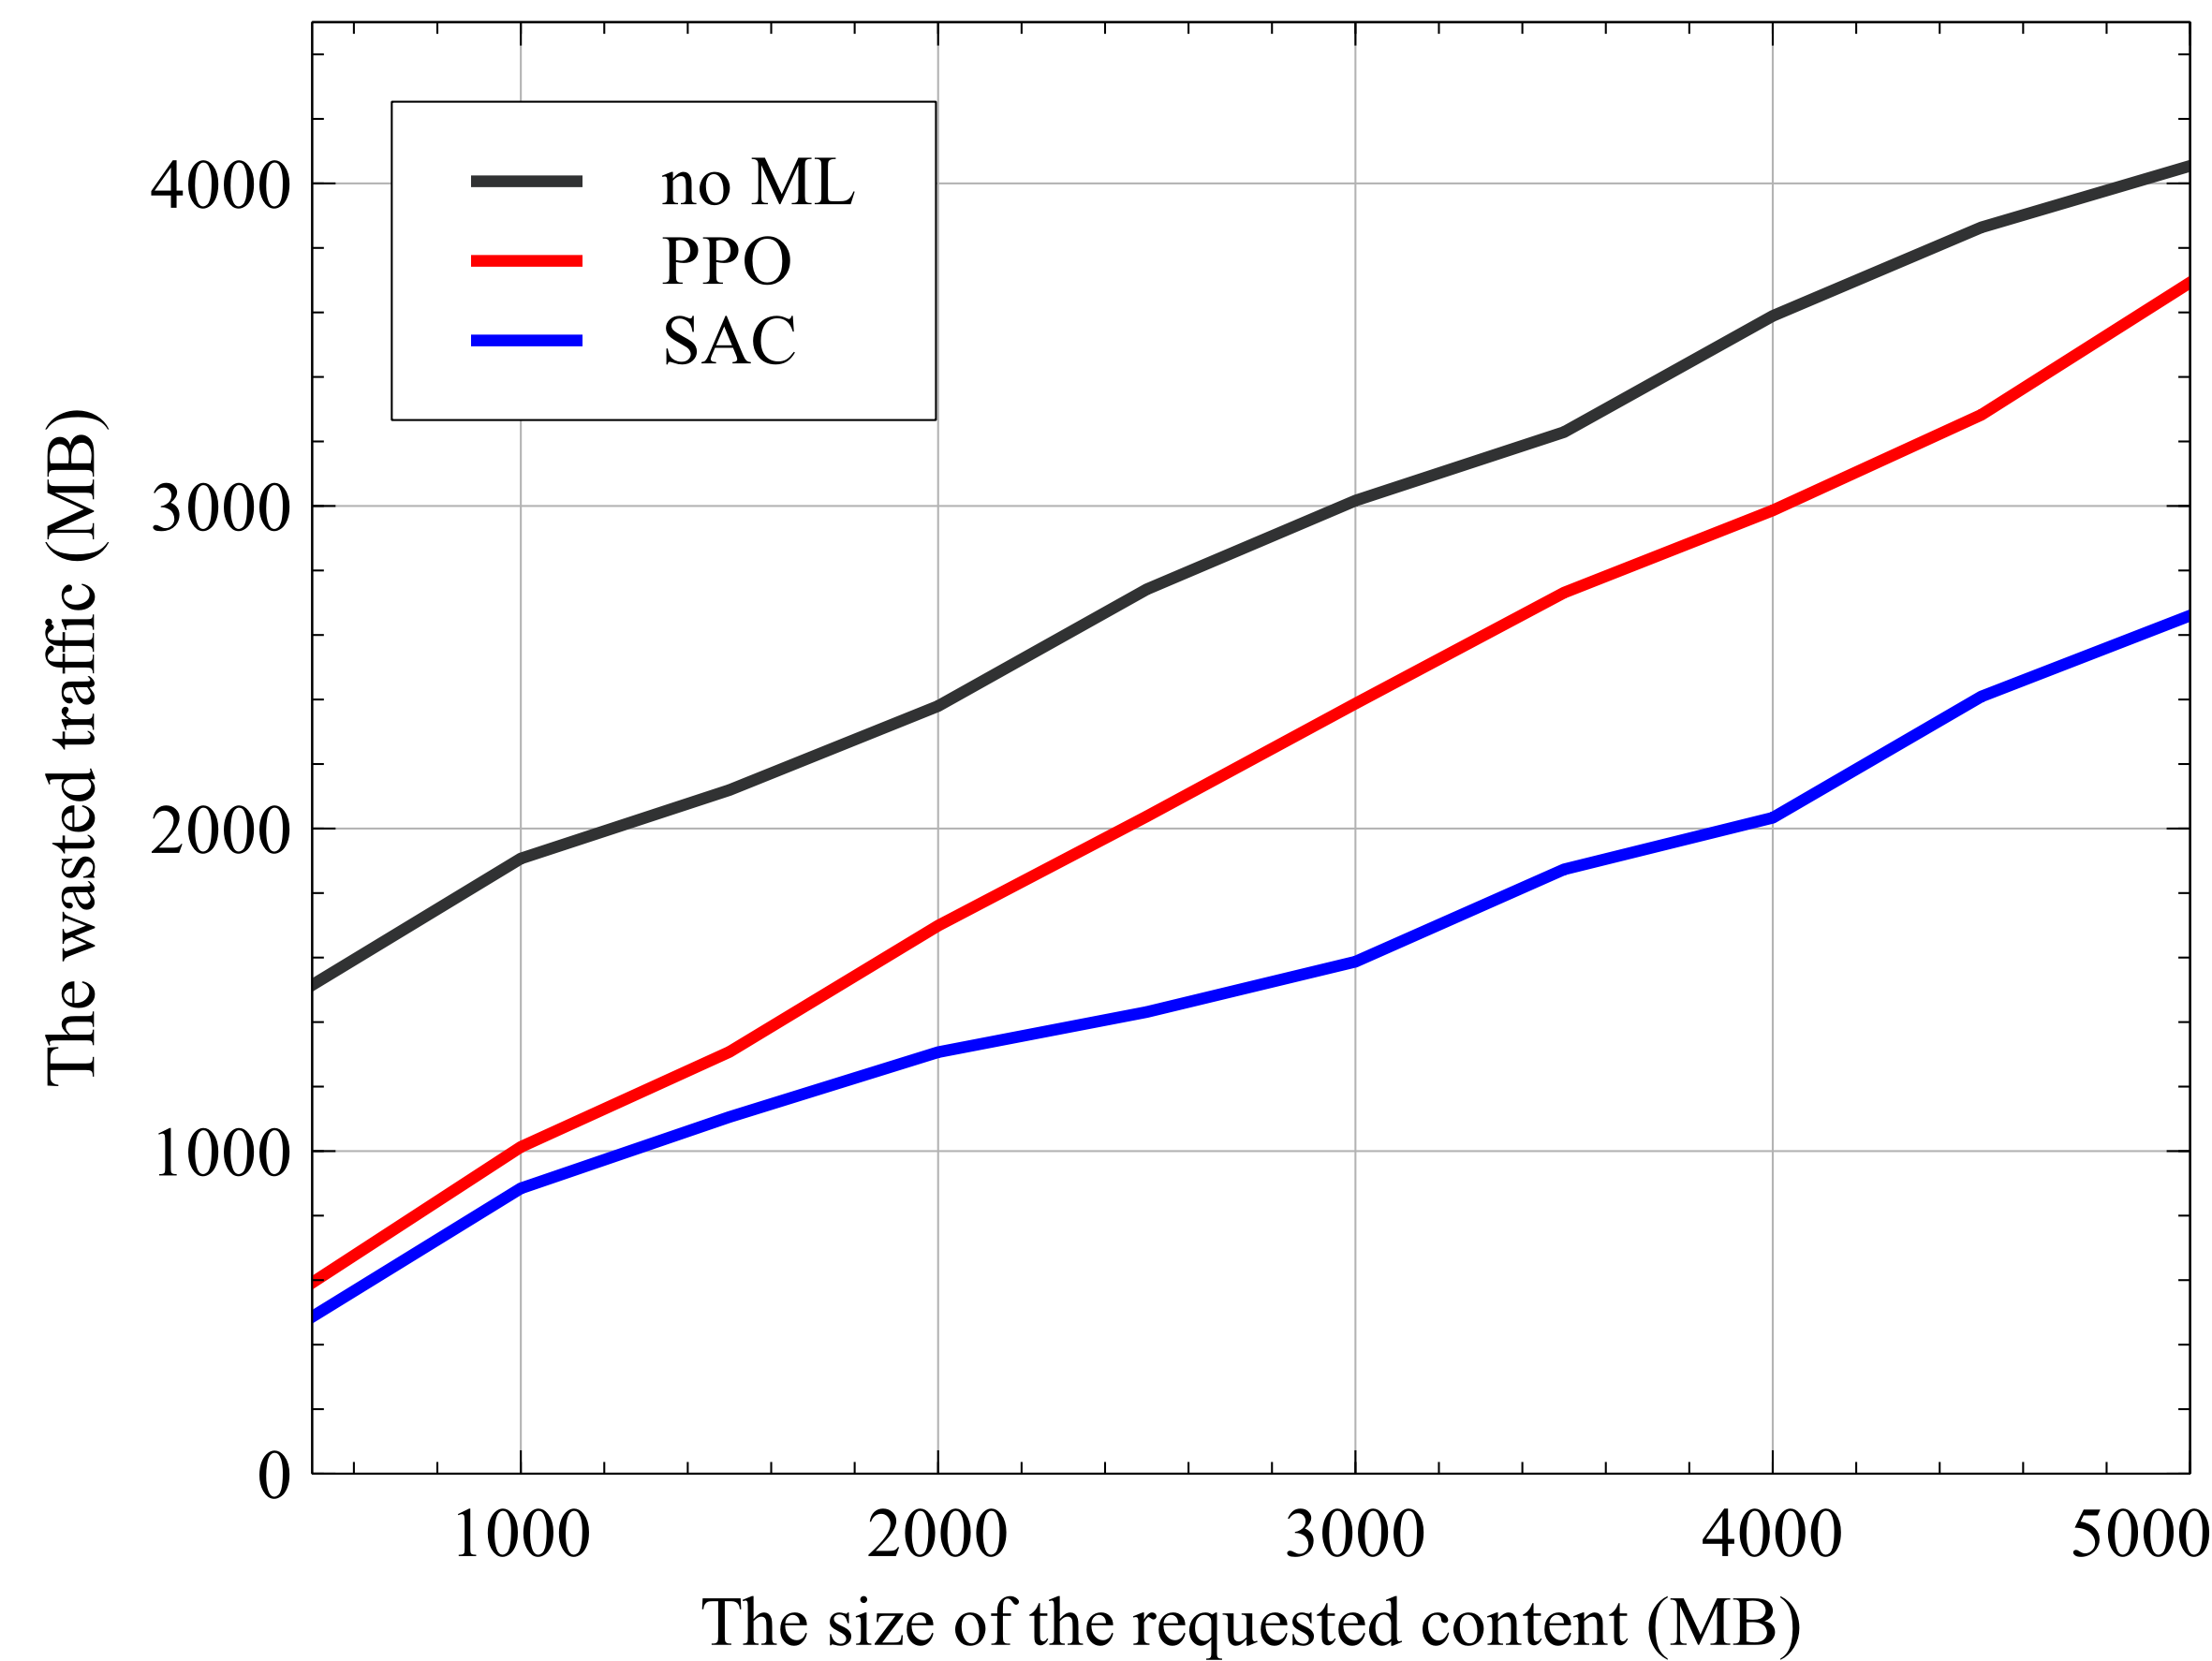
\includegraphics[width=0.45\textwidth]{./graphs/Results_10.png}
    \label{fig:g41}}
    \subfigure[]{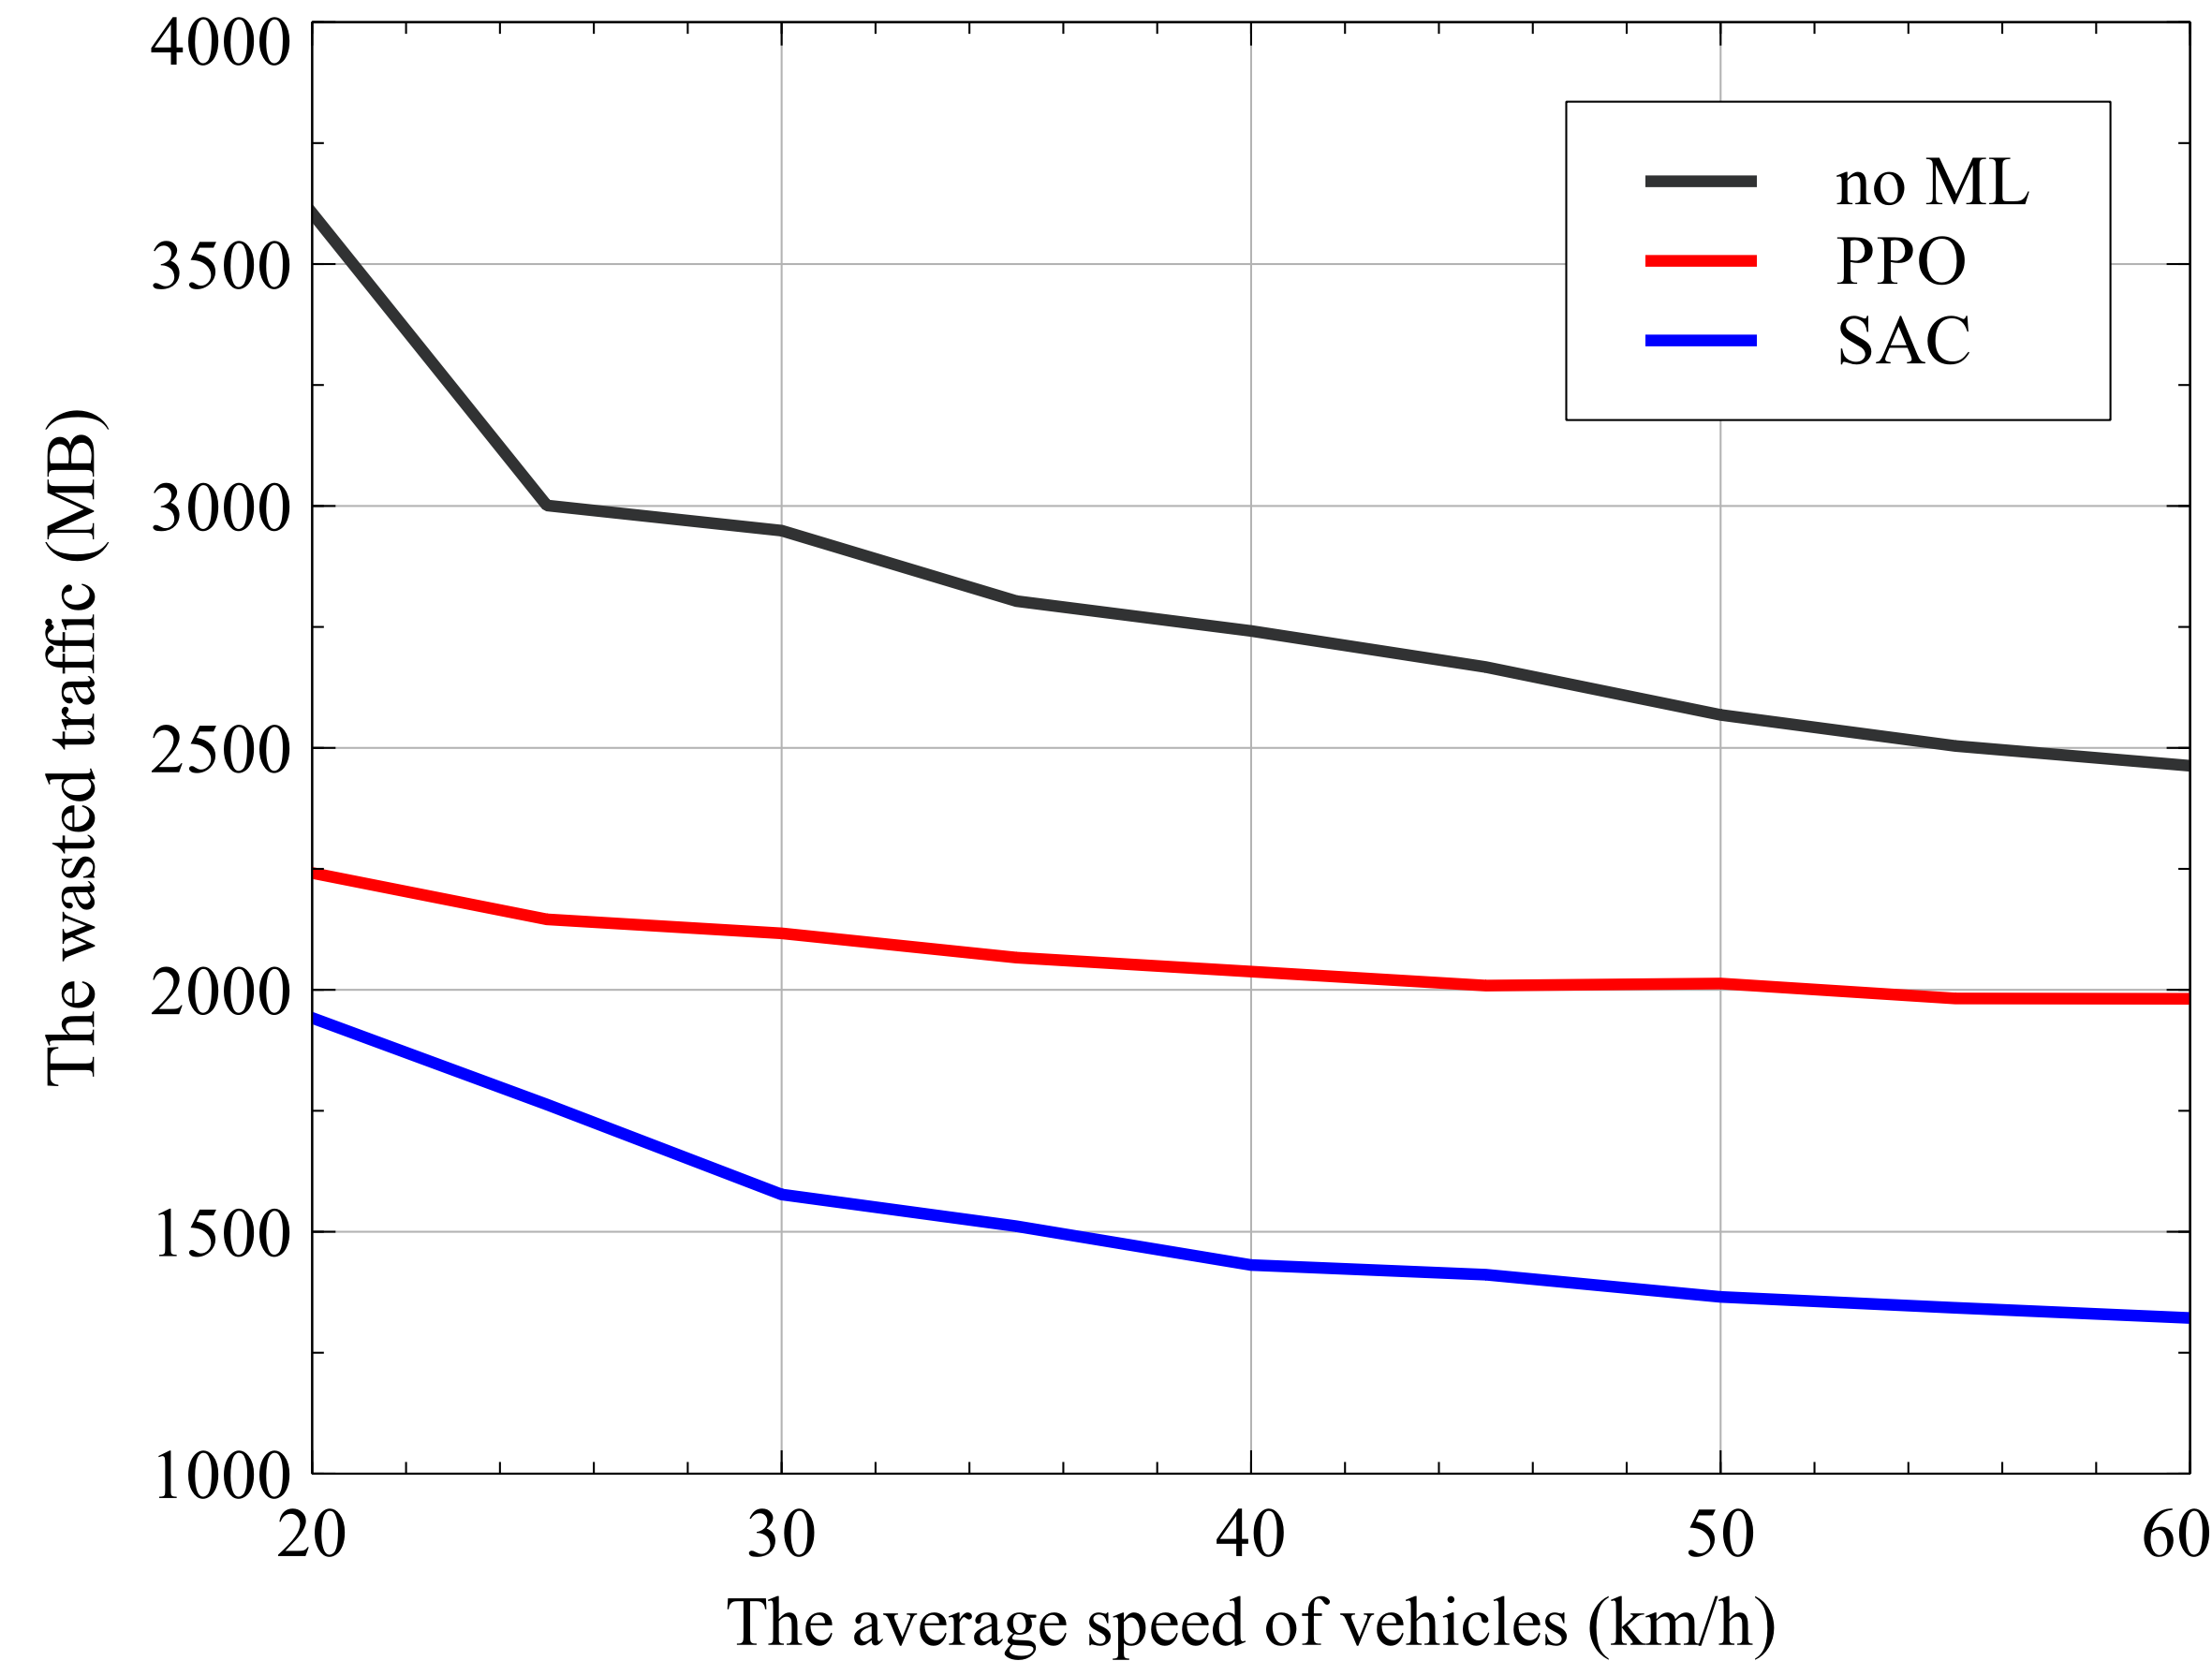
\includegraphics[width=0.45\textwidth]{./graphs/Results_12.png}
    \label{fig:g42}}
    \subfigure[]{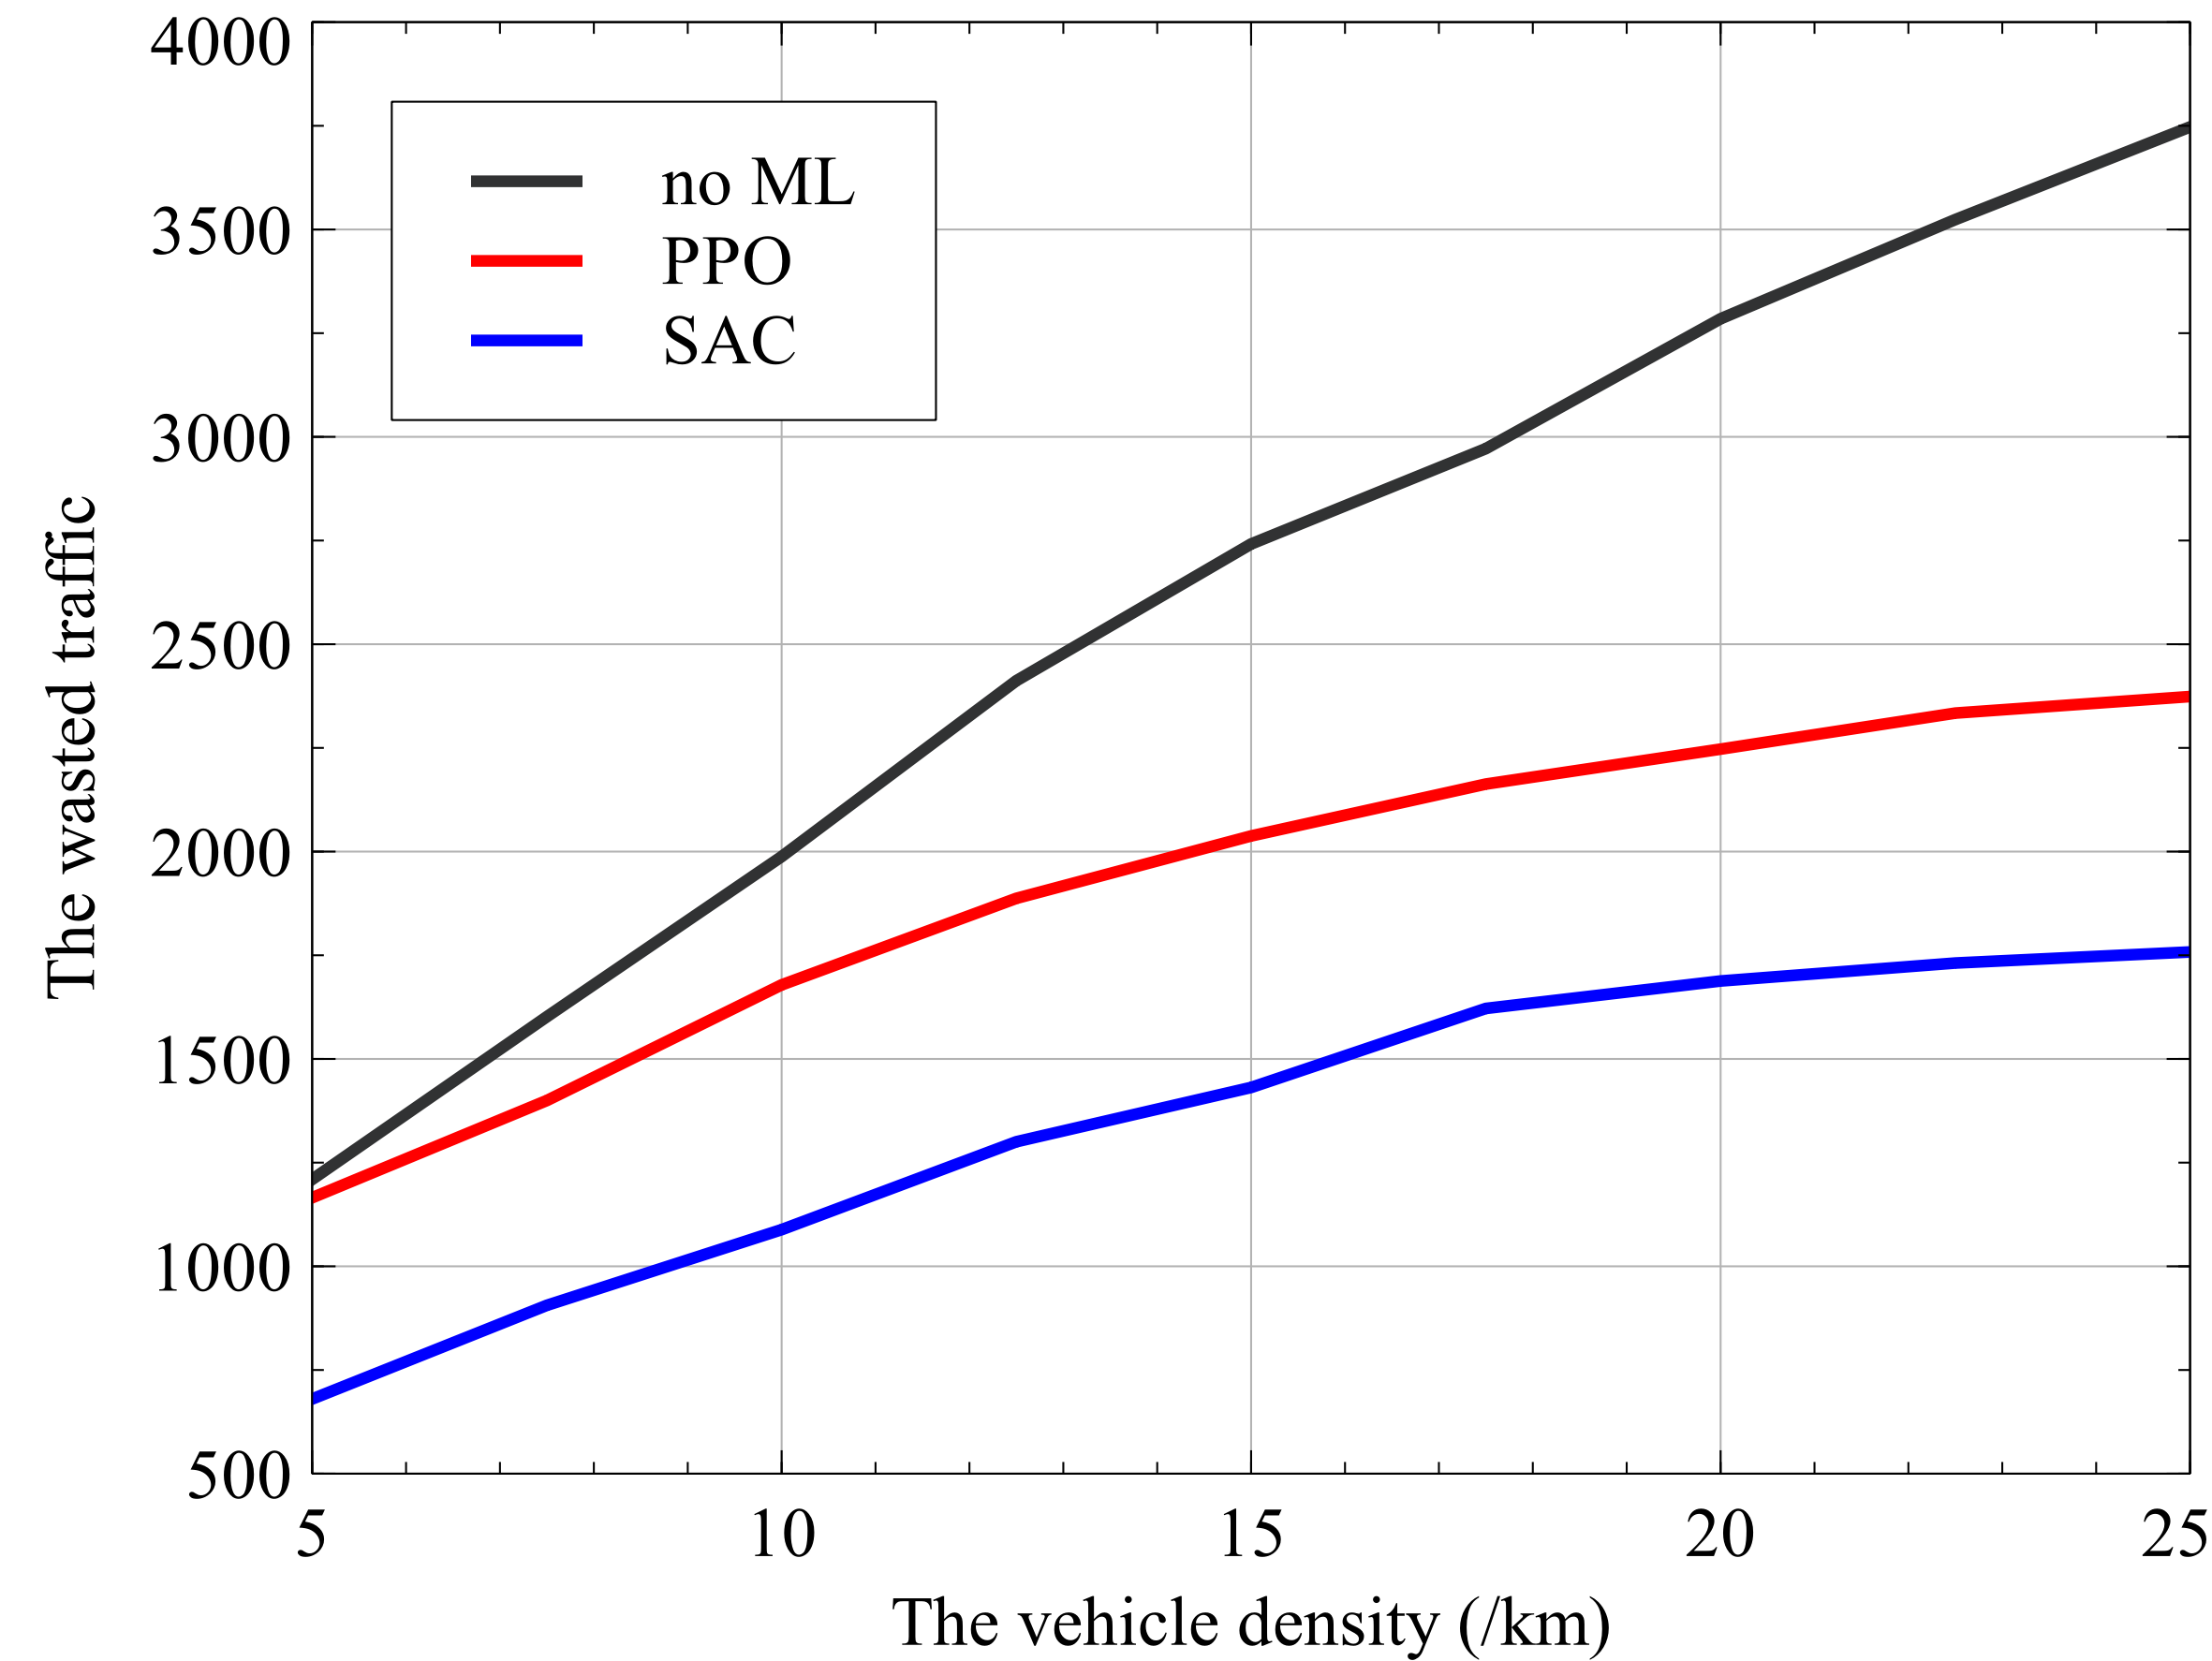
\includegraphics[width=0.45\textwidth]{./graphs/Results_14.png}
    \label{fig:g43}}
    \caption{The wasted traffic according to (a) the size of the requested content, (b) the average speed of vehicles, and (c) the vehicle density.}
\end{figure}
\section{Discussion} \label{sec.disc}
In this section, we discuss the positioning of our study, its potential for integration with other domains, and the direction for future practical implementation, addressing the scalability and robustness of the proposed SAC-PVS scheme.

\subsection{Significance of Snapshot-based SAC-PVS and future model evolution}
Some may argue that our scheme merely applies the standard SAC algorithm to a vehicular network problem.
However, the main contribution of this study lies not in the modification of the RL algorithm itself, but in the novel architectural design of applying RL to V2V precaching in a snapshot-based manner rather than a time-series inference model.
Unlike typical time-series approaches (e.g., transformers or LSTMs) that require continuous data streams and impose significant overhead on network resources and delay sensitivity, our proposed scheme makes inference based on a distinct snapshot of the network state at the moment a request is generated.
To realize this, we meticulously designed the state, action, and reward functions specifically for the V2V precaching context and developed a compatible communication protocol that enables the exchange of these designed parameters between vehicles and RSUs.
This study provides foundational experimental proof that a snapshot-based RL approach can effectively optimize precaching without the burden of continuous monitoring.
By validating this feasibility, our work opens the door to future research exploring more sophisticated state-of-the-art models or customized deep learning architectures tailored for specific vehicular environments.
While SAC was chosen for its robustness in dynamic environments through entropy regularization, exploring other continuous control algorithms—such as TD3, DDPG, or Attention-based PPO—within our proposed framework remains a promising direction for further optimizing the inference engine.


\subsection{Scalability and integration with heterogeneous networks}
While this paper focuses on V2V networks, the principles of the SAC-PVS framework are broadly applicable to other network resource allocation and scheduling problems.
The proposed scheme for dynamic node selection and content sizing can be extended to Unmanned Aerial Vehicle~(UAV)-assisted communication, edge server selection, and dynamic service placement in mobile edge computing (MEC).
For instance, in a UAV-assisted scenario\cite{Liu2024}, the precaching vehicle in our model could be replaced with a UAV, with the action space adapted to include factors such as UAV altitude or energy constraints.
We envision developing an integrated framework that unifies these heterogeneous components, leveraging the communication protocols established here to comprehensively manage diverse network resources.

\subsection{Practical implementation and real-world validation}
The primary objective of this paper was to experimentally validate the applicability of SAC-based decision-making in a V2V precaching environment.
To this end, we adopted simulated mobility models to control environmental variables and isolate the performance impact of the algorithm.
We recognize that real-world deployment introduces additional complexities, such as irregular road topologies, fluctuating signal interference, and unpredictable driver behaviors.
Having demonstrated the theoretical and simulation-based effectiveness of our specific state-action-reward design, our future work will focus on bridging the gap to practicality.
We intend to integrate real-world mobility traces~(e.g., using SUMO \cite{SUMO}  with real city maps) and empirical content consumption datasets~(e.g., MovieLens~\cite{MovieLens}) to test the robustness of our protocol.
Additionally, we aim to optimize RSU deployment and refine protocol parameters to handle extreme conditions, such as ultra-sparse vehicle densities or high-mobility highways.
It ensures the system's reliability in practical~CIoV~deployments.

\section{Conclusions} \label{sec.conc}
In this paper, we presented the SAC-based Precaching Vehicle Selection (SAC-PVS) scheme, an innovative approach aimed at mitigating content delivery delays and improving network efficiency in Content-centric Internet of Vehicles (CIoV) environments, particularly in outage zones with limited RSU coverage.
Our framework operates in two stages: the precaching vehicle selection stage, which leverages a hierarchical reward function to accurately identify the most suitable vehicles for precaching, and the precaching quantity decision stage, which determines the optimal quantity of content to be precached by each selected vehicle.

We experimentally validated the feasibility of applying a snapshot-based RL approach for V2V precaching, distinguishing it from traditional time-series inference models.
By designing a tailored state-action-reward structure and a compatible communication protocol, the system optimizes vehicle selection and content allocation in real-time, effectively managing the dynamic nature of CIoV without continuous monitoring overhead.
Simulation results, conducted using a grid-based Manhattan mobility model show that SAC-PVS significantly reduces content download delays and minimizes wasted traffic compared to baseline approaches such as PPO and no ML schemes.
These improvements were particularly pronounced under conditions of high vehicle speeds, dense traffic, and large content requests in CIoV.


\section*{Author contributions}
Youngju Nam: Methodology, software, writing-original draft; Yongje Shin: Conceptualization, methodology, writing-review and editing; Hyeonseok Choi: Visualization, validation, writing-review and editing; Euisin Lee: Supervision, writing-review and editing. All authors have read and approved the final version of the manuscript for publication.

\section*{Use of Generative-AI tools declaration}
The authors declare that they have not used Artificial Intelligence (AI) tools in the creation of this~article.

\section*{Acknowledgments}
This work was supported by a National Research Foundation of Korea (NRF) grant funded by the Korean government (Ministry of Science and ICT (MSIT)) (No. 2022R1A2C1010121).

\section*{Conflict of interest}
The authors declare that they have no competing interests.
\newpage
\begin{thebibliography}{999}
\bibitem{yuan2018} Q. Yuan, H. Zhou, J. Li, Z. Liu, F. Yang, X. S. Shen,  Toward efficient content delivery for automated driving services: An edge computing solution, \emph{IEEE Network}, \textbf{32} (2018), 80--86. \doilink{https://doi.org/10.1109/MNET.2018.1700105}

\bibitem{Ericsson} Ericsson mobility report. Available online: \url{https://www.ericsson.com/en/reports-and-papers/mobility-report/dataforecasts/mobile-traffic-forecast/} (Accessed: February 3, 2026).
\bibitem{Pranav2019} P. K. Singh, S. K. Nandi, S. Nandi, A tutorial survey on vehicular communication state of the art, and future research directions, \emph{Veh. Commun.}, \textbf{18} (2019), 100164. \doilink{https://doi.org/10.1016/j.vehcom.2019.100164}

\bibitem{Reichardt2002} D. Reichardt, M. Miglietta, L. Moretti, P. Morsink, W. Schulz,  \emph{CarTALK 2000: Safe and comfortable driving based upon inter--vehicle--communication}, In: Intelligent Vehicle Symposium, 2002. IEEE, Versailles, France, \textbf{2} (2002), 545--550. \doilink{https://doi.org/10.1109/IVS.2002.1188007}

\bibitem{Li2017} Z. Li, Y. Chen, D. Liu, X. Li, Performance analysis for an enhanced architecture of IoV via content--centric networking, \emph{EURASIP J. Wirel. Comm.}, \textbf{2017} (2017), 124. \doilink{https://doi.org/10.1186/s13638-017-0905-4}

\bibitem{Khan2024} M. T. R. Khan, Y. Z. Jembre, M. M. Saad, S. H. Bouk, S. H. Ahmed, D. Kim, Proactive content retrieval based on value of popularity in content-centric internet of vehicles,  \emph{IEEE T. Intell. Transp.}, \textbf{25} (2024), 8514--8526. \doilink{https://doi.org/10.1109/TITS.2024.3378669} 

\bibitem{Ahmed2018} S. Ahmed, D. Mu, D. Kim, Improving Bivious Relay Selection in Vehicular Delay Tolerant Networks, \emph{IEEE T. Intell. Transp.}, \textbf{19} (2018), 987--995. \doilink{https://doi.org/10.1109/TITS.2018.2791925}

\bibitem{Wang2021} R. Wang, Z. Kan, Y. Cui, D. Wu, Y. Zhen, Cooperative Caching Strategy With Content Request Prediction in Internet of Vehicles, \emph{IEEE Internet  Things}, \textbf{8} (2021), 8964--89751. \doilink{https://doi.org/10.1109/JIOT.2021.3056084}


\bibitem{Guo2017} T. Guo, C. Li, Z. Miao, W. Dong, X. Su, \emph{Prefetching-based content download for highway vehicular ad hoc networks},  In: 2017 IEEE/CIC International Conference on Communications in China (ICCC), Qingdao, China, 2017, 1--6. \doilink{https://doi.org/10.1109/ICCChina.2017.8330346}

\bibitem{Wang2017} Y. Wang, Y. Liu, J. Zhang, H. Ye, Z. Tan,  Cooperative Store–Carry–Forward scheme for intermittently connected vehicular networks,  \emph{IEEE T. Veh. Technol.}, \textbf{66} (2017),  777--784. \doilink{https://doi.org/10.1109/TVT.2016.2536059}

\bibitem{Nam2023} Y. Nam, J. Bang, H. Choi, Y. Shin, S. Oh, E. Lee.  Multiple precaching vehicle selection scheme based on set ranking in intermittently connected vehicular networks,  \emph{Sensors}, \textbf{23} (2023), 5800. \doilink{https://doi.org/10.3390/s23135800}

\bibitem{Zhang2024} Y. Zhang, R. Wang, Y. Wang, M. Chen, M. Guizani,  Diversity-driven proactive caching for mobile networks,  \emph{IEEE T. Mobile Comput.}, \textbf{23} (2024), 7878--7894. \doilink{https://doi.org/10.1109/TMC.2023.3340733}

\bibitem{Chen2024} G. Chen, J. Sun, Y. Zhou, Q. Zeng, F. Shen,  A novel proactive cache decision algorithm based on prior knowledge and aerial cloud assistance in internet of vehicles,  \emph{IEEE T. Netw. Sci. Eng.}, \textbf{11} (2024), 5280--5297. \doilink{https://doi.org/10.1109/TNSE.2024.3433544}

\bibitem{Jacobson2009} V. Jacobson, D. K. Smetters, J. D. Thornton, M. F. Plass, N. H. Briggs, R. L. Braynard, \emph{Networking named content},  In: Proceedings of the 5th international conference on Emerging networking experiments and technologies, Rome, Italy, 2009, 1--12. \doilink{https://doi.org/10.1145/1658939.1658941}

\bibitem{zhang2014} L. Zhang, A. Afanasyev, J. Burke, V. Jacobson, K. Claffy, P. Crowley, et al.,  Named data networking,  \emph{ACM SIGCOMM Comp. Com.}, \textbf{44} (2014), 66--73. \doilink{https://doi.org/10.1145/2656877.2656887}

\bibitem{Amadeo2012} M. Amadeo, C. Campolo, A. Molinaro,  \emph{Content--centric vehicular networking: An evaluation study},  In: 2012 Third International Conference on The Network of the Future (NOF), Tunis, Tunisia, 2012,  1--5. \doilink{https://doi.org/10.1109/NOF.2012.6463994}

\bibitem{Su2017} Z. Su, Y. Hui, Q. Yang,  The next generation vehicular networks: A content-centric framework,  \emph{IEEE Wirel. Commun.},  \textbf{24} (2017), 60--66. \doilink{https://doi.org/10.1109/MWC.2017.1600195WC}

\bibitem{Wang2019} X. Wang, X. Wang,  Vehicular content--centric networking framework,  \emph{IEEE Syst. J.}, \textbf{13} (2019), 519--529. \doilink{https://doi.org/10.1109/JSYST.2018.2875918}

\bibitem{Ikram2021} I. U. Din, B. Ahmad, A. Almogren, H. Almajed, I. Mohiuddin, J. J. P. C. Rodrigues,   Left--right--front caching strategy for vehicular networks in ICN--based internet of things,  \textit{IEEE Access}, \textbf{9} (2021), 595--605. \doilink{https://doi.org/10.1109/ACCESS.2020.3046887}

\bibitem{Zhao2021} G. Ahani, D. Yuan,  \emph{On optimal proactive and retention--aware caching with user mobility},  In: 2018 IEEE 88th Vehicular Technology Conference (VTC-Fall), Chicago, IL, USA, 2018, 1--5. \doilink{https://doi.org/10.1109/VTCFall.2018.8691020}

\bibitem{Banerjee2022} C. Liang, F. R. Yu, N. Dao, G. Senarath, H. Farmanbar,  \emph{Enabling adaptive data prefetching in 5G mobile networks with edge caching},  In: 2018 IEEE Global Communications Conference (GLOBECOM), Abu Dhabi, United Arab Emirates, 2018, 1--6. \doilink{https://doi.org/10.1109/GLOCOM.2018.8647443}

\bibitem{Yao2020} L. Yao, Z. Li, W. Peng, B. Wu, W. Sun,  \emph{A pre-caching mechanism of video stream based on hidden Markov model in vehicular content centric network},  In: 2020 3rd International Conference on Hot Information-Centric Networking (HotICN), Hefei, China, 2020,  53--58. \doilink{https://doi.org/10.1109/HotICN50779.2020.9350830}

\bibitem{Zhang2020} Z. Zhang, C. H. Lung, M. S. Hilaire, I. Lambadaris,  Smart proactive caching: Empower the video delivery for autonomous vehicles in ICN-based networks,  \emph{IEEE T. Veh. Technol.}, \textbf{69} (2020), 7955--7965. \doilink{https://doi.org/10.1109/TVT.2020.2994181}

\bibitem{Mahmood2019} A. Mahmood, C. E. Casetti, C. F. Chiasserini, P. Giaccone, J. Härri,  The RICH prefetching in edge caches for in-order delivery to connected cars,  \emph{IEEE T. Veh. Technol.}, \textbf{68} (2019), 4--18. \doilink{https://doi.org/10.1109/TVT.2018.2879850}

\bibitem{Abani2017} N. Abani, T. Braun, M. Gerla,  \emph{Proactive caching with mobility prediction under uncertainty in information-centric networks}, In: Proceedings of the 4th ACM Conference on Information-Centric Networking, Berlin, Germany, 2017, 88--97. \doilink{https://doi.org/10.1145/3125719.3125728}

\bibitem{Zhao2023} W. Zhao, C. Wu, R. Zhong, K. Shi, X. Xu,  \emph{Edge computing and caching optimization based on PPO for task offloading in RSU-assisted IoV},  In: 2023 IEEE 9th World Forum on Internet of Things (WF-IoT), Aveiro, Portugal, 2023, 01--06. \doilink{https://doi.org/10.1109/WF-IoT58464.2023.10539436}

\bibitem{Wang2023} S. Wang, Q. Zhu, H. Huang, Y. Lei, W. Zhan, H. Duan,  \emph{Deep reinforcement learning based real-time proactive edge caching in intelligent transportation system},  In: 2023 8th International Conference on Cloud Computing and Big Data Analytics (ICCCBDA), Chengdu, China, 2023,  162--166. \doilink{https://doi.org/10.1109/ICCCBDA56900.2023.10154769}

\bibitem{Feng2023} B. Feng, C. Feng, D. Feng, Y. Wu, X. G. Xia,  Proactive content caching scheme in urban vehicular networks,  \emph{IEEE Trans. Commun.}, \textbf{71} (2023), 4165--4180. \doilink{https://doi.org/10.1109/TCOMM.2023.3277530}

\bibitem{Azzalini} A. Azzalini, A. Capitanio,  \emph{The skew--normal and related families}, Cambridge University Press, 2013.

\bibitem{Zipf} L. Breslau, P. Cao, L. Fan, G. Phillips, S. Shenker,  \emph{Web caching and Zipf--like distributions: Evidence and implications},  In: IEEE INFOCOM '99. Conference on Computer Communications. Proceedings. Eighteenth Annual Joint Conference of the IEEE Computer and Communications Societies. The Future is Now (Cat. No.99CH36320), New York, USA, 1999, 126--134. \doilink{https://doi.org/10.1109/INFCOM.1999.749260}

\bibitem{SB3} A. Raffin, A. Hill, A. Gleave, A. Kanervisto, M. Ernestus, N. Dormann, Stable-baselines3: Reliable reinforcement learning implementations, \emph{J. Mach. Learn. Res.}, \textbf{22} (2021), 1--8. %\doilink{}

\bibitem{Liu2024} B. Liu, Y. Cai, D. Li, K. Lin, G. Xu, A hybrid ARO algorithm and key point retention strategy trajectory optimization for UAV path planning, \emph{Drones},  \textbf{8} (2024), 644. \doilink{https://doi.org/10.3390/drones8110644}

\bibitem{SUMO} P. A. Lopez, M. Behrisch, L. B. Walz, J. Erdmann, Y. Fl{\"o}tter{\"o}d, R. Hilbrich,  et al., \emph{Microscopic traffic simulation using SUMO}, In: 2018 21st International Conference on Intelligent Transportation Systems (ITSC), Maui, HI, USA, 2018, 2575--2582. \doilink{https://doi.org/10.1109/ITSC.2018.8569938}

\bibitem{MovieLens} F. M. Harper,   J. A. Konstan,  The MovieLens datasets: History and context,  \emph{ACM T. Interact. Intel.}, \textbf{5} (2015), 1--19. \doilink{https://doi.org/10.1145/2827872}
\end{thebibliography}

\end{document}
